\documentclass[twoside]{book}

\newcommand{\arxiv}[2]{#1} %for arxiv
%\newcommand{\arxiv}[2]{#2} %for kdp

\usepackage{problems}
\usepackage[colorlinks=true,
citecolor=black,
linkcolor=black,
anchorcolor=black,
filecolor=black,
menucolor=black,
urlcolor=black,
pdftitle={PIGTIKAL: puzzles in geometry that I know and love},
pdfsubject={Geometry},
pdfauthor={Anton Petrunin},
]{hyperref}

\geometry{top=0.9in, bottom=0.9in,inner=0.9in, outer=0.7in, paperwidth=6in, paperheight=9in}
%\geometry{top=0.9in, bottom=0.9in,left=0.9in, right=0.9in, paperwidth=6in, paperheight=9in}%without bleed
%\geometry{top=1.025in, bottom=1.025in,inner=.9in, outer=1.025in, paperwidth=6.125in, paperheight=9.25in}%with bleed
\makeindex

\arxiv{}{\usepackage[x-1a]{pdfx}} 

\begin{document}
%\pagestyle{empty}\renewcommand\includegraphics[2][{}]{}

%\title{\huge PIGTIKAL}
%\subtitle{(puzzles in geometry\\
%that I know and love)}
%\author{\Large Anton Petrunin}
%\date{}
%\maketitle

\begin{titlepage}
\fontfamily{pbk}\selectfont  
    \vspace*{4.5\baselineskip}
    \centering

\centering
\vspace*{3mm}
{\huge PIGTIKAL} \\[0em]
{\huge (puzzles in geometry\\
that I know and love)}\\[14mm]
{\Large Anton Petrunin} 
\par
\vspace*{55mm}
{\large Association for Mathematical Research\\[0mm]
Monographs Volume 2}
\par
\vspace*{14mm}
\includegraphics[angle=0, scale=.17]{cover/amr-small.jpg}
\end{titlepage}

\noindent
Anton Petrunin\\
Department of Mathematics\\
The Pennsylvania State University\\
University Park, PA 16802\\
USA\\[20mm]
\noindent
AMR Monographs\\
Editorial Board:

\qquad George Andrews

\qquad Colin Adams

\qquad 
Eric Friedlander

\qquad 
Robert Ghrist

\qquad 
Joel Hass

\qquad 
Robion Kirby

\qquad 
Alex Kontorovich

\qquad 
Sergei Tabachnikov\\
[30mm]
\noindent{\includegraphics[scale=0.5]{pics/by-sa}
\vspace*{1mm}
\\
Copyright © 2022 by Anton Petrunin\\
This work is licensed under a CC BY-SA 4.0 license\\
To view a copy of this license, visit:\\
\texttt{https://creativecommons.org/licenses/by-sa/4.0/legalcode}\\
\null\vfill
\noindent %ISBN : 979-8694260817\\
\texttt{arXiv:0906.0290v18}\\[3mm]
Association for Mathematical Research

\qquad Davis, CA; Jenkintown PA\\[3mm]
\noindent Cover design: Robert Ghrist


\thispagestyle{empty}
\tableofcontents
\thispagestyle{empty}

\newpage
\thispagestyle{empty}
\section*{Preface}

This collection is about ideas, and it is not about theory.
An idea might feel more comfortable in a suitable theory,
but it has its own life and history, and it can speak for itself.

I am collecting these problems for fun, 
but they might be used to improve 
the problem-solving skills in geometry.
Every problem has a short elegant solution ---
this gives a hint which was not available
when the problem was discovered.

%Here is one reason to read this collection.
%In your research you might face a problem that can be solved by an easy trick.
%It is a pity to miss such a trick especially since it is easy and fun to learn.
%On the other hand, learning a theory is harder and not as much fun, but if you miss it, then likely you can get help from a friend, so usually it does not stop you.

\parbf{How to read it.}
Open at a random chapter, make sure you like the practice problem --- if yes try to solve a random problem in the chapter.
A semisolution is given at the end of the chapter,
but think before reading,
otherwise it will not help. 

Some problems are marked by $\circ$, $*$, $+$ or $\sharp$.
\begin{itemize}
\item[$\circ$] --- easy problem;%\easy
\item[$*$] --- the solution requires at least two ideas;%\hard
\item[$+$] --- the solution requires knowledge of a theorem;%\thm
\item[$\sharp$] --- there are interesting solutions based on different ideas.%\many
\end{itemize}

\parbf{Acknowledgments.} 
I want to thank everyone who helped me;
here is an incomplete list:
Stephanie Alexander,
Ilya Alexeev,
Miroslav Ba\v{c}\'{a}k, 
Christopher Croke,
Bogdan Georgiev,
Sergei Gelfand,
Jouni Luukkainen,
Alexander Lytchak,
Andrei Malyutin, 
Rostislav Matveyev, 
Dmitri Panov, 
Peter Petersen, 
Idzhad Sabitov,
Thomas Sharpe,
Serge Tabachnikov, and
Sergio Zamora Barrera.

This collection is partly inspired by \emph{connoisseur's collection} of puzzles of Peter Winkler \cite[][]{winkler}.
Many problems were suggested on MathOverflow~\cite[][]{One-step}.

This work was partially supported by the following grants:
NSF grants DMS 
0103957,
0406482,
0905138,
1309340,
2005279,
Simons Foundation grants 
245094 and 584781,
and
Minobrnauki grant 075-15-2022-289.


\chapter{Curves}


Recall that a \index{curve}\emph{curve} is a continuous map defined on real interval
and 
a \index{closed curve}\emph{closed curve} is a continuous map defined on a circle.
If the map is injective then the curve is called \index{simple curve}\emph{simple}.

In this chapter we consider only plane and spherical curves.
We assume that the reader is familiar with related definitions including 
length of curve 
and its curvature.
The necessary material is covered in a the first couple of lectures 
of a standard introduction to differential geometry, 
see \cite[][\S26--27]{hilbert-cohn-vossen}
or  
\cite[][Chapter 1]{toponogov-curves-and-surfaces}.

\medskip

We give a practice problem with a solution, 
after that you are on your own.

\subsection*{Spiral}

The following problem states that 
if you drive on the plane and turn the steering wheel to the right all the time,
then you will not be able to come back to the same place.

\begin{pr}{}{Problem}\label{spiral}
Assume $\gamma$ is a smooth regular plane curve with strictly monotonic curvature. 
Show that $\gamma$ has no self-intersections.
\end{pr}

\parit{Solution.}
Without loss of generality we may assume that the curve is parametrized by its length and its
curvature decreases.

Let $z(t)$ be the center of osculating circle at $\gamma(t)$
and $r(t)$ is its radius.
That is 
\begin{align*}
z(t)&=\gamma(t)+\tfrac{\ddot\gamma(t)}{|\ddot\gamma(t)|^2},
&
r(t)&=\tfrac{1}{|\ddot\gamma(t)|}.
\end{align*}

\begin{wrapfigure}{o}{25 mm}
\begin{lpic}[t(-0 mm),b(-2 mm),r(0 mm),l(0 mm)]{pics/kneser-log(1)}
\end{lpic}
\end{wrapfigure}

Straightforward calculations show that
\[|\dot z(t)|\le \dot r(t).\]
It follows that the osculating discs are nested;
that is, 
$D_{t_1}\supset D_{t_0}$ for $t_1>t_0$.
Hence the result follows.\qeds

This problem gives a continuous analog of the Leibniz's test for alternating series.
It was considered by Peter Tait in \cite{tait}
and later rediscovered by Adolf Kneser in \cite{kneser};
see also \cite{ovsienko-tabachnikov}.

%%%%%%%%%%%%%%%%%%%%%%%%%%%%%%%%%%%%%%%%%%%%%%%%%
{

\begin{wrapfigure}[6]{r}{27 mm}
\begin{lpic}[t(-5 mm),b(0 mm),r(0 mm),l(0 mm)]{pics/moon-in-puddle(1)}
\lbl{14.5,22.5;$F$}
\end{lpic}
\end{wrapfigure}

\subsection*{The moon in the puddle}

\begin{pr}{}{The moon in the puddle}\label{moon-in-puddle}
A smooth closed simple plane curve with curvature less than $1$ bounds a figure $F$. 
Prove that $F$ contains a disc of radius~$1$.
\end{pr}

}

%%%%%%%%%%%%%%%%%%%%%%%%%%%%%%%%%%%%%%%%%%%%%%%%%
\subsection*{A spring in a tin}

\begin{pr}{\many}{A spring in a tin}\label{A spring in a tin} 
Let $\alpha$ be a closed smooth immersed curve
inside a unit disc. 
Prove that the average absolute curvature of $\alpha$ is at least $1$, with
equality if and only if $\alpha$ is the unit circle possibly traversed more than once.
\end{pr}

%%%%%%%%%%%%%%%%%%%%%%%%%%%%%%%%%%%%%%%%%%%%%%%%%
\subsection*{A curve in a sphere}
\label{A curve in a sphere}

\begin{pr}{\many}{A curve in a sphere} 
Show that if a closed curve on the unit sphere intersects every equator then it has length at least $2\cdot\pi$.
\end{pr}

%%%%%%%%%%%%%%%%%%%%%%%%%%%%%%%%%%%%%%%%%%%%%%%%%
{

\begin{wrapfigure}{r}{30 mm}
\begin{lpic}[t(2 mm),b(-1 mm),r(0 mm),l(0 mm)]{pics/tangent-eq(1)}
\end{lpic}
\end{wrapfigure}

\subsection*{Oval in oval}


\begin{pr}{}{Oval in oval}\label{Oval in oval} 
Consider two closed smooth strictly convex planar curves, one inside the other. 
Show that there is a chord of the outer curve, which is tangent to the inner curve at its midpoint.
\end{pr}

}

%%%%%%%%%%%%%%%%%%%%%%%%%%%%%%%%%%%%%%%%%%%%%%%%%
\subsection*{Capture a sphere in a knot\hard}

The following problem states that one can not capture a sphere in a knot.

The precice formulation use the notion of smooth isotopy of knots;
that is, one parameter of embeddings 
\[f_t\:\mathbb{S}^1\z\to \RR^3,\ \  t\in[0,1]\] 
such that the map $[0,1]\times \mathbb{S}^1\to\RR^3$ is smooth.


\begin{pr}{}{Capture a sphere in a knot}\label{Capture a sphere in a knot}
Let $B$ be the closed unit ball in $\RR^3$
and $f\:\mathbb{S}^1\z\to \RR^3\backslash B$ be a knot.
Show that there is a smooth isotopy 
$$f_t\:\mathbb{S}^1\to \RR^3\backslash B,\ \ \ t\in [0,1],$$ 
such that $f_0=f$,
the length of $f_t$ does not increase in $t$
and $f_1(\mathbb{S}^1)$ can be separated from $B$ by a plane.
\end{pr}

%%%%%%%%%%%%%%%%%%%%%%%%%%%%%%%%%%%%%%%%%%%%%%%%%
\subsection*{Linked circles}

\begin{pr}{}{Linked circles}\label{linked-circles}
Suppose that two linked  simple closed curves in $\RR^3$
lie at a distance at least $1$ from each other.
Show that the length of each curve is at least $2\cdot\pi$.
\end{pr}

%%%%%%%%%%%%%%%%%%%%%%%%%%%%%%%%%%%%%%%%%%%%%%%%%
\subsection*{Surrounded area}

\begin{pr}{\easy}{Surrounded area}\label{Surrounded area}
Let $\gamma_1,\gamma_2\:\mathbb S^1\to\RR^2$ be two simple closed plane curves.
Assume 
\[|\gamma_1(v)-\gamma_1(w)|\le|\gamma_2(v)-\gamma_2(w)|\]
for any $v,w\in \mathbb S^1$.
Show that the area surrounded by $\gamma_1$ does not exceed the area surrounded by $\gamma_2$. 
\end{pr}

%%%%%%%%%%%%%%%%%%%%%%%%%%%%%%%%%%%%%%%%%%%%%%%%%
\subsection*{Fat curve}

\begin{pr}{\easy}{Fat curve}\label{Fat curve}
Construct a simple plane curve with positive Lebesgue measure.
\end{pr}


%%%%%%%%%%%%%%%%%%%%%%%%%%%%%%%%%%%%%%%%%%%%%%%%%
\subsection*{Crooked circle}

\begin{pr}{}{Crooked circle}\label{Crooked circle} 
Construct 
a bounded open disc in $\RR^2$ 
such that 
its boundary contains no simple curve.
\end{pr}

%%%%%%%%%%%%%%%%%%%%%%%%%%%%%%%%%%%%%%%%%%%%%%%%%
\subsection*{Rectifiable curve}

In the following problem we use the notion of 
\index{Hausdorff measure}\emph{Hausdorff measure} for the compact subsets in the plane.
Fix a compact set $X\subset\RR^2$ and $\alpha>0$.
Given $\delta>0$ consider the value
\[h(\delta)=\inf\left\{\,\sum_i(\diam X_i)^\alpha\,\right\}\]
where the infimum is taken for all coverings of $X$ by $\{X_i\}$
such that $\diam X_i<\delta$ for each $i$.

Note that the function $\delta\mapsto h(\delta)$ does is not decreasing in $\delta$.
In particular, the limit $h$ of $h(\delta)$ as $\delta\to0$ is defined, possibly infinite.
This value $h$ is called $\alpha$-dimensional Hausdorff measure of $X$.

\begin{pr}{}{Rectifiable curve}\label{Rectifiable curve}
Assume $X$ is a compact connected set in $\RR^2$
with finite 1-dimensional Hausdorff measure. 
Show that $X$ can be represented as the image of a rectifiable curve.
\end{pr}

%%%%%%%%%%%%%%%%%%%%%%%%%%%%%%%%%%%%%%%%%%%%%%%%%
\subsection*{Typical convex functions}

Recall that \index{G-delta set}\emph{G-delta set} is defined as a countable intersection of open sets.
According to \index{Baire category theorem}\emph{Baire category theorem}, 
in a complete metric spaces,
any intersection of countable collection of dense open set 
has to be dense.

In particular, in a complete metric spaces, 
the intersection of a finite or countable collection of G-delta dense sets is also G-delta dense. 
The later means that G-delta dense sets contains {}\emph{most} of the points of a complete metric space. 
This is the meaning of the word {}\emph{most} used in the following problem.

\begin{pr}{\easy}{Typical convex functions}\label{Most of the convex functions}
Consider the space of continuous convex functions defined on $[0,1]$,
equipped with the metric induced by sup norm.

Show that most of these functions have vanishing the second derivative at any point where it is defined.
\end{pr}


\section*{Semisolutions}

%%%%%%%%%%%%%%%%%%%%%%%%%%%%%%%%%%%%%%%%%%%%%%%%%%

\parbf{The moon in the puddle.}
Consider the {\it cut locus} $T$
of $F$ with respect to $\partial F$;
it is defined as the closure
of the set of points $x\in F$ 
such that there are two or more points in $\partial F$ which minimize distance to $x$.

\begin{wrapfigure}{o}{28 mm}
\begin{lpic}[t(-0 mm),b(-0 mm),r(0 mm),l(0 mm)]{pics/moon-in-puddle-sol(1)}
\lbl[t]{21,10;$\partial F$}
\lbl[br]{8.5,30,;{\small $T$}}
\lbl[tr]{6,4;{\small $z_0$}}
\end{lpic}
\end{wrapfigure}

Note that after a small perturbation
of $\partial F$ we may assume that
$T$ is a graph embedded in
$F$ with finite number of edges.

Note that $T$ is a
deformation retract of $F$.
The retraction can be obtained by moving each point $y\in F\setminus T$ to $T$
along the geodesic from the closest point to $y$ on $\partial F$ which pass through $y$.

In particular, $T$ is a tree.
Therefore $T$  has
at least two end vertices;
Denote one of them by $z$.

Prove that the disc of radius $1$ centered at $z$ lies completely in $F$.\qeds

The problem discussed by German Pestov and Vla\-di\-mir Ionin in \cite{pestov-ionin}.
An other solution via curve shortening flow 
was given by Konstantin Pankrashkin in  \cite{pankrashkin}.
The statement still holds if the curve fails to be smooth at one point.
A spherical version of the later statement 
was used by Dmitri Panov and me 
in \cite{panov-petrunin-ramification}.

The 3-dimensional analog of this statement does not hold.
Namely, there is a smooth embedding $\mathbb{S}^2\hookrightarrow \RR^3$ 
with all the principle curvatures between $-1$ and $1$
such that it does not surround a ball of radius 1.
Such example can be obtained by fattening a nontrivial contractible 2-complex in $\RR^3$ 
\cite[the Bing's house constructed in][will do the job]{bing}.
This problem is discussed by Vladimir Lagunov in \cite{lagunov-2} 
and it was generalized to Riemannian manifolds with boundary by Stephanie Alexander and Richard Bishop \cite[see][]{alexander-bishop}.

A similar argument shows that
for any point $p\in (\mathbb S^2,g)$ there is a minimizing geodesic $[pq]$ with conjugate ends.
On the other hand, 
for $(\mathbb S^3,g)$ this is not true.
In fact, 
there are Riemannian metrics on $\mathbb{S}^3$ 
without minimizing geodesics with conjugate ends,
yet more restrictive example is given in \cite{buser-gromoll}.



 


%%%%%%%%%%%%%%%%%%%%%%%%%%%%%%%%%%%%%%%%%%%%%%%%%%
\parbf{A spring in a tin.}
Let $\alpha$ be a closed curve in the unit disc;
denote by $\ell$ its length.

Let us equip the plane with complex coordinates so that $0$ is the center of the unit disc.
We can assume that $\alpha$ equipped with $\ell$-periodic parametrization by length.

Consider the curve $\beta(t)=t-\tfrac{\alpha(t)}{\dot\alpha(t)}$.
Note that 
\[\beta(t+\ell)=\beta(t)+\ell\] 
for any $t$.
In particular 
\[\length (\beta|_{[0,\ell]}) 
\ge 
|\beta(\ell)-\beta(0)|
=
\ell.\]

Note that 
\begin{align*}
|\dot\beta(t)|&=|\tfrac{\alpha(t)\cdot\ddot\alpha(t)}{\dot\alpha(t)^2}|\le
\\
&\le|\ddot\alpha(t)|.
\end{align*}
Since $|\ddot\alpha(t)|$ is the curvature of $\alpha$ at $t$,
we get the result.\qeds

The statement was originally proved 
by Istv\'an F\'ary in \cite{fary};
number of different proofs are discussed by Serge Tabachnikov in \cite{tabachnikov}, see also \cite[19.5 in ][]{fuchs-tabachnikov}.

If instead of a disc, 
we have a region bounded by closed convex curve $\gamma$, 
then it is still true that the average curvature of $\alpha$ is at least as big as average curvature of $\gamma$. 
The proof was given by Jeffrey Lagarias
and Thomas Richardson in \cite{lagarias-richardson}, see also \cite{nazarov-petrov}.


%%%%%%%%%%%%%%%%%%%%%%%%%%%%%%%%%%%%%%%%%%%%%%%%%%
\parbf{A curve in a sphere.} 
We give two solutions, both by contradiction.
Assume that $\alpha$ is a closed curve in $\mathbb{S}^2$ of length $2\cdot\ell$ which intersects each equator.
Let us present two solutions.

\parit{A solution with the Crofton formula.}
Note that we can assume that $\alpha$ is a broken line.

Given a unit vector $u$ denote by $e_u$ the equator with pole at $u$.
Let $k(u)$ the number of intersections
of the $\alpha$ and $e_u$.

Note that for almost all $u\in \mathbb{S}^2$, the value $k(u)$ is even.
Since each equator intersects $\alpha$, we get $k(u)\ge 2$ for almost all $u$.

Then we get
\begin{align*}
2\cdot\ell&=\tfrac14\cdot\int\limits_{\mathbb{S}^2}k(u)\cdot\, d_u\area\ge 
\\
&\ge\tfrac12\cdot\area\mathbb{S}^2=
\\
&=2\cdot\pi.
\end{align*}
The first identity above is called \index{Crofton formula}\emph{Crofton formula}.
To prove this identity, consider a curve formed by on geodesic segment
and
then sum up the obtained identities for all segments in $\alpha$.\qeds

\parit{A solution by symmetry.}
Let $\check\alpha$ be a sub-arc of $\alpha$ of length $\ell$, with endpoints $p$ and $q$.  
Let $z$ be the midpoint of a minimizing geodesic $[pq]$ in $\mathbb{S}^2$.  

Let $r$ be a point of intersection of $\alpha$ with the equator with pole at $z$.  
Without loss of generality we may assume that $r\in\check\alpha$. 

The arc $\check\alpha$ together with its reflection in $z$ 
form a closed curve of length $2\cdot \ell$ 
that passes through $r$ and its antipodal point $r^{*}$.
Therefore 
\[\ell=\length \check\alpha\ge |r-r^{*}|_{\mathbb S^2}=\pi.\]
Here $|r-r^{*}|_{\mathbb S^2}$ 
denotes the angle metric in the sphere $\mathbb S^2$.\qeds


The problem was suggested by Nikolai Nadirashvili.

%%%%%%%%%%%%%%%%%%%%%%%%%%%%%%%%%%%%%%%%%%%%%%%%%%
%%%%%%%%%%%%%%%%%%%%%%%%%%%%%%%%%%%%%%%%%%%%%%%%%%
\begin{wrapfigure}{r}{51 mm}
\begin{lpic}[t(-3 mm),b(-3 mm),r(0 mm),l(0 mm)]{pics/tangent-eq-sol(1)}
\lbl[tr]{20,5;$u$}
\lbl[rt]{18,15;$r$}
\lbl[rt]{26,6;$l$}
\lbl[bl]{25,10;$x_u$}
\end{lpic}
\end{wrapfigure}

\parbf{Oval in oval.}
Show that the chord which minimizes (or maximizes) the ratio, 
in which it divides the bigger oval, 
solves the problem.\qeds


\parit{Alternative solution.}
Given a unit vector $u$, denote by $x_u$ the point on the inner curve
with outer normal vector $u$.
Draw a chord of outer curve which is tangent to the inner curve at $x_u$;
denote by $r=r(u)$ and $l=l(u)$ the lengths of this chord at the right and left from $x_u$.


Arguing by contradiction, assume $r(u)\ne l(u)$ for any $u\in\mathbb{S}^1$.
Since the functions $r$ and $l$ are continuous,
we can assume that 
$$r(u)>l(u)\ \ \text{for any}\ \ u\in\mathbb{S}^1.\leqno{({*})}$$

Prove that
each of the following two integrals 
\begin{align*}
\tfrac12\cdot\int\limits_{\mathbb{S}^1}r^2(u)\cdot du
\quad\text{and}\quad
\tfrac12\cdot\int\limits_{\mathbb{S}^1}l^2(u)\cdot du
\end{align*}
gives 
the area between the curves.
In particular, 
the integrals are equal to each other. 
The latter contradicts $({*})$.\qeds



This is a problem of Serge Tabachnikov \cite[see][]{tabachnikob-mi}.
A closely related, so called {}\emph{equal tangents problem} is discussed by the same author in \cite{tabachnikov-tan}.

%%%%%%%%%%%%%%%%%%%%%%%%%%%%%%%%%%%%%%%%%%%%%%%%%%
\parbf{Capture a sphere in a knot.}
We can assume that the knot is given by a diagram on the sphere.

Fix a M\"obius transformation $\mathbb{S}^2\to\mathbb{S}^2$ which is not an isometry.
Denote by $u$ its conformal factor. 
Since the M\"obius transformation preserves total area, 
we get 
$$\frac1{\area \mathbb{S}^2}\cdot\int\limits_{\mathbb{S}^2} u^2=1.$$ 
Therefore, 
$$\frac1{\area \mathbb{S}^2}\cdot\int\limits_{\mathbb{S}^2} u<1.$$ 
It follows that after a suitable rotation of $\mathbb{S}^2$, 
the length of the knot decreases.

The same way one gets 
a continuous one parameter family of M\"obius transformations which moves the knot in a hemisphere 
and allows the ball to escape. \qeds


This is a problem of Zarathustra Brady, 
the given solution is based on the idea of David Eppstein \cite[see][]{zeb}.



%%%%%%%%%%%%%%%%%%%%%%%%%%%%%%%%%%%%%%%%%%%%%%%%%%
\parbf{Linked circles.} 
Denote the linked circels by $\alpha$ and $\beta$.

Fix a point $x\in\alpha$. 
Note that one can find another point $x^{*}\in\alpha$ such that the interval 
$[xx^{*}]$ intersects $\beta$, say at the point $z$. 
Otherwise we can move each point of $\alpha$ along the line segment to $x$.
This deformation of $\alpha$ will not cross $\beta$;
the latter contradicts that $\alpha$ and $\beta$ are linked. 


Consider the curve $\alpha^{*}$ which is the central projection of $\alpha$ 
from $z$ onto the unit sphere around $z$;
clearly
$$\length \alpha\ge \length\alpha^{*}.$$

Note that $\alpha^{*}$ passes through two antipodal points of the sphere;
therefore 
$$\length \alpha^{*}\ge 2\cdot\pi.$$
Hence the result follows.\qeds


This is the simplest case of so called \index{Gehring's problem}\emph{Gehring's problem}. 
The solution above was given by Michael Edelstein and Binyamin Schwarz in \cite{edelstein-schwatz};
later the same solution was rediscovered few times.





%%%%%%%%%%%%%%%%%%%%%%%%%%%%%%%%%%%%%%%%%%%%%%%%%%
\parbf{Surrounded area.}
Denote by $C_1$ and $C_2$ the compact regions bounded by $\gamma_1$ and $\gamma_2$ correspondingly.

By Kirszbraun theorem, 
any short map $X\to \RR^2$ defined on $X\subset \RR^2$
can be extended to a short map on the whole $\RR^2$.
In particular, there is a short map $f\:\RR^2\to\RR^2$ 
such that $f(\gamma_2(v))=f(\gamma_1(v))$ for any $v\in\mathbb S^1$.

Note that $f(C_2)\supset C_1$.
Whence the statement follows.\qeds


The Kirszbraun theorem appears in his thesis \cite[see][]{kirszbraun}
and reproved later by Frederick Valentine in \cite{valentine}.


%%%%%%%%%%%%%%%%%%%%%%%%%%%%%%%%%%%%%%%%%%%%%%%%%%
\begin{wrapfigure}{r}{40 mm}
\begin{lpic}[t(-5 mm),b(-2 mm),r(0 mm),l(0 mm)]{pics/serpinski-cemetery(1)}
\end{lpic}
\end{wrapfigure}

%%%%%%%%%%%%%%%%%%%%%%%%%%%%%%%%%%%%%%%%%%%%%%%%%%
\parbf{Fat curve.}
To solve the problem, you can modify your favorite space filling curve 
keeping its area nearly the same 
and removing the self-intersections.

It works for the \index{Sierpi\'nski curve}\emph{Sierpi\'nski curve} 
which can be constructed as a limit of 
recursively defined sequence of curves;
the 8th iteration is on the diagram.\qeds 

The existence of such curves was observed 
by William Osgood in \cite{osgood}.


%%%%%%%%%%%%%%%%%%%%%%%%%%%%%%%%%%%%%%%%%%%%%%%%%%
\parbf{Crooked circle.}
A continuous function $f\:[0,1]\to [0,1]$
will be called $\eps$-crooked 
if $f(0)=0$, $f(1)=1$ 
and for any segment $[a,b]\subset [0,1]$ 
one can choose $a\le x\le y\le b$ 
such that
\[|f(y)-f(a)|\le\eps\ \ \text{and}\ \ |f(x)-f(b)|\le\eps.\]

A sequence of $\tfrac1n$-crooked maps can be constructed recursively. 
Guess the construction from the diagram.



\begin{center}
\begin{lpic}[t(-0 mm),b(4 mm),r(0 mm),l(0 mm)]{pics/crooked(1)}
\lbl[t]{8,0;$\eps=\tfrac12$}
\lbl[t]{33,0;$\eps=\tfrac13$}
\lbl[t]{57,0;$\eps=\tfrac14$}
\lbl[t]{80,0;$\eps=\tfrac15$}
\end{lpic}
\end{center}


Start with the unit circle, 
$\gamma_0(t)=(\cos \tfrac{t}{2\cdot\pi},\sin \tfrac{t}{2\cdot\pi})$.
Construct recursively a sequence of simple closed curves $\gamma_n\:[0,1]\to\RR^2$.
Such that $\gamma_{n+1}$ runs outside of the disc bounded by $\gamma_n$
and 
\[|\gamma_{n+1}(t)-\gamma_n\circ f_n(t)|<\eps_n,\]
for some $\eps_n$-crooked function $f_n\:[0,1]\to[0,1]$.

\begin{wrapfigure}{o}{46 mm}
\begin{lpic}[t(-2 mm),b(0 mm),r(0 mm),l(0 mm)]{pics/circrooked(1)}
\lbl[tr]{35,33;$\gamma_0$}
\lbl[bl]{38,36;$\gamma_1$}
\end{lpic}
\end{wrapfigure}

On the diagram you see an attempt to draw the first iteration.

Denote by $D$ the union of all discs bounded by $\gamma_n$.
Show that $D$ is homeomorphic to an open disc 
and for the right choice of the $\eps_n$ the set $D$ is bounded and its
boundary contains no simple curves.\qeds


The proof repeats the construction of pseudo-arc 
given by Bronis\l{}aw Knaster in \cite{knaster}.
Let us list a few problems which can be solved the same way.
\begin{itemize}
\item {\it Construct three disjoint non-empty open sets in $\RR$ which have the same boundary.}
\item {\it Construct three open discs in $\RR^2$ which have the same boundary.}
(This example are called \index{lakes of Wada}\emph{lakes of Wada}; it is  described by Kuniz\^{o} Yoneyama in \cite{yoneyama}.)
\item {\it Construct a Cantor set in $\RR^3$ with non simply connected complement.}
(This example was is called  \index{Antoine's necklace}\emph{Antoine's necklace};
it is constructed in \cite{antoine}.)
\item {\it Construct an open set in $\RR^3$ with fundamental group isomorpphic to the additive group of rational numbers.}
\end{itemize}
For more advanced examples check 
Whitehead manifold, 
\emph{Dogbone space}, 
\emph{Casson handle};
see also the problem ``Conic neighborhood'' on page \pageref{Conic neighborhood}.





%%%%%%%%%%%%%%%%%%%%%%%%%%%%%%%%%%%%%%%%%%%%%%%%%%
\parbf{Rectifiable curve.}
The 1-dimensional Hausdorff measure will be denoted as $\mathcal{H}_1$. 

Set $L=\mathcal{H}_1(K)$.
Without loss of generality, we may assume that $K$ has diameter $1$.

Assume that $0<\eps<\tfrac12$.
Prove that 
\[\mathcal{H}_1(B(x,\eps)\cap K)\ge\eps\leqno(*)\]
for any $x\in K$.

Let $x_1,\dots, x_n$ be a maximal set of points in $K$ such that 
\[|x_i-x_j|\z\ge\eps\] for all $i\ne j$. 
From $(*)$ we have $n\le2\cdot L/\eps$.

Construct a curve $\gamma_\eps$ such that (1) $\gamma_\eps$ is passing through all $x_i$, (2) $\length\gamma_\eps\le10\cdot L$ and (3) $\gamma_\eps$ lies in $\eps$-neighborhood of $K$.
We can assume that $\gamma_\eps$ is parametrized by length.

The needed curve can be obtained by passing to 
a partial limit of $\gamma_\eps$
 as $\eps\to 0$. \qeds


This problem was given by Kenneth Falconer
in his book \cite[Exercise 3.5 in][]{falconer}.



%%%%%%%%%%%%%%%%%%%%%%%%%%%%%%%%%%%%%%%%%%%%%%%%%%
\parbf{Typical convex functions.}
Denote by $\mathfrak{F}$ the space of convex all functions defined on $[0,1]$ with the sup-norm.
Note that $\mathfrak{F}$ is a complete metric space.

Prove that if a function $f\in\mathfrak{F}$ has nonzero derivative at some point then there is $\eps>0$ such that
\[|f-g|> \frac{\eps}{n^{23}}\]
if $g\in\mathfrak{F}$  can be presented as a maximum of $n$ linear functions.

Note that there is a countable set of piecewise linear convex $g_1,g_2,\dots$ functions which is everywhere dense in $\mathfrak{F}$.
Denote by $n_i$ the number of linear intervals of $g_i$.
For any positive integer $k$,
consider the set $\Omega_k\subset\mathfrak{F}$ defined as 
\[\Omega_k
=
\set{|f-g_i|<\frac1{k\cdot n_i^{23}}}{\text{for some}\ i}.\]

From above we get that if the second derivative of $f$ does not vanishing at some point then $f\notin\Omega_k$ for large $k$. 

Note that $\Omega_k$ is open and everywhere dense in $\mathfrak{F}$.
Therefore 
\[\Omega=\bigcap_k\Omega_k\]
is a G-delta dense set.
Hence the statement follows.\qeds
  


This problem states that typical convex functions is very far from what we used to work with.

This is a typical answer for such question --- typicaly we do not see the typical objects.
For example, according to the result of 
Bernd Kirchheim, 
Emanuele Spadaro  
and 
L{\'a}szl{\'o} Sz{\'e}kelyhidi proved in \cite{KSS}
a typical 1-Lipschitz maps from the plane to itself preserves the length of all curves.
The same way one could show that the typical open discs in the plane contain no simple curves in their boundary, 
although the construction of one such is not trivial, 
see ``Crooked circle'' above.

More similar problems are surveyed by Tudor Zamfirescu in \cite{zamfirescu}.








\csname @openrightfalse\endcsname
\chapter{Surfaces}

We assume that the reader is familiar with smooth surfaces and the related definitions
including intrinsic metric, 
geodesics,
convex and saddle surfaces
as well as different types of curvature.
An introductory course in differential geometry should cover all necessary background material 
[see for example \S28--29 in \ncite{hilbert-cohn-vossen}
or  
\ncite{toponogov-curves-and-surfaces}].



%%%%%%%%%%%%%%%%%%%%%%%%%%%%%%%%%%%%%%%%%%%%%%
{

\begin{wrapfigure}{r}{27 mm}
\vskip4mm
\centering
\includegraphics{mppics/pic-202}
\end{wrapfigure}


\subsection*{Convex hat}
\label{Convex hat}

\begin{pr}
Suppose that a plane $\Pi$ cuts from a smooth closed convex surface $\Sigma$ a disk $\Delta$.
Assume that the reflection of $\Delta$ with respect to $\Pi$ lies inside of $\Sigma$.
Show that $\Delta$ is \index{convex set}\emph{convex} with respect to the intrinsic metric  of $\Sigma$;
that is, 
if both ends of a minimizing geodesic in $\Sigma$ 
lie in $\Delta$,
then the entire geodesic lies in $\Delta$.
\end{pr}

}


\parit{Semisolution.}
Assume the contrary,
then there is a minimizing geodesic $\gamma\not\subset\Delta$ with ends $p$ and $q$ in $\Delta$.

Without loss of generality, we may assume that only one arc of $\gamma$ lies outside of $\Delta$.
Reflection of this arc  with respect to $\Pi$ together with the remaining part of $\gamma$ forms another curve $\hat\gamma$ from $p$ to $q$;
it runs partly along $\Sigma$ 
and partly outside $\Sigma$,
but does not get inside $\Sigma$.
Note that
\[\length\hat\gamma=\length\gamma.\]


Denote by $\bar\gamma$ the closest point projection of $\hat\gamma$ on $\Sigma$.
Since $\Sigma$ is convex, the closest point projection decreases the length.
Therefore 
the curve $\bar\gamma$ lies in $\Sigma$, 
it has the same ends as $\gamma$,
and
\[\length\bar\gamma<\length\gamma.\]
This means that $\gamma$ is not length minimizing, 
a contradiction.\qeds

%%%%%%%%%%%%%%%%%%%%%%%%%%%%%%%%%%%%%%%%%%%%%%

{


\begin{wrapfigure}{r}{39 mm}
\vskip0mm
\centering
\includegraphics{mppics/pic-204}
\end{wrapfigure}

\subsection*{Involute of geodesic}
\label{Involute of  geodesic}

\begin{pr}
Let $\Sigma$ be a smooth closed strictly convex surface 
in $\RR^3$ 
and $\gamma\:[0,\ell]\z\to \Sigma$ a unit-speed minimizing geodesic.
Set $p\z=\gamma(0)$, $q=\gamma(\ell)$ and 
$$p_t=\gamma(t)-t\cdot\gamma'(t),$$ 
where $\gamma'(t)$ denotes the velocity vector of $\gamma$ at $t$.
\end{pr}

}
\vskip-\medskipamount
\textit{Show that for any $t\in (0,\ell)$,
one {}\emph{cannot see}  $q$ from $p_t$;
that is, the line segment $[p_tq]$ intersects $\Sigma$ at a point distinct from $q$.}

%%%%%%%%%%%%%%%%%%%%%%%%%%%%%%%%%%%%%%%%%%%%%%
\subsection*{Simple geodesic}
\label{Simple geodesic}

\begin{pr}
Let $\Sigma$ be a complete unbounded convex surface in $\mathbb R^3$.
Show that there is a two-sided infinite geodesic in $\Sigma$ with no self-intersections.
\end{pr}

Let us review a couple of statements 
about Gauss curvature which might help to solve the problem \cite[see \S28 in][for more details]{hilbert-cohn-vossen}.

If $\Sigma$ is a convex surface in $\RR^3$ then its Gauss curvature is nonnegative.

Assume that a simply connected region $\Omega$ in the surface $\Sigma$ is bounded by a closed broken geodesic $\gamma$.
Denote by $\kappa(\Omega)$ the integral of the Gauss curvature over $\Omega$.

For any point $p\in\Sigma$ consider the outer unit normal vector $n(p)\z\in\mathbb{S}^2$.
Then 
\begin{align*}
\kappa(\Omega)&=\area[n(\Omega)]
\intertext{and by the Gauss--Bonnet formula}
\kappa(\Omega)&=2\cdot\pi-\sigma(\gamma),
\end{align*}
where $\sigma(\gamma)$ denotes the sum of the signed exterior angles of $\gamma$.
In particular,  $|\sigma(\gamma)|\le2\cdot\pi$.





%%%%%%%%%%%%%%%%%%%%%%%%%%%%%%%%%%%%%%%%%%%%%%
\subsection*{Geodesics for birds}
\label{liberman}

The \index{total curvature}\emph{total curvature} of a space curve $\gamma$ is defined as the integral of its curvature.
That is, if a curve $\gamma\:[a,b]\to\RR^3$ has unit speed parametrization, 
then its total curvature equals 
\[\int\limits_a^b|\gamma''(t)|\cdot dt,\]
the vector $\gamma''(t)$ is called \index{curvature vector}\emph{curvature vector} and its length $|\gamma''(t)|$ is the \index{curvature}\emph{curvature} of $\gamma$ at time $t$.
The above definition makes sense for $C^{1,1}$ smooth curves,
that is, in the case when $\gamma'(t)$ is locally Lipschitz;
in this case the curvature $|\gamma''(t)|$ is defined almost everywhere.

The \index{geodesic}\emph{geodesics} in the following problem are defined as the curves locally minimizing the length;
that is, any sufficiently short arc of the curve containing a given value of the parameter is length minimizing.

\begin{pr}
Let $f\:\RR^2\to\RR$ be a smooth $\ell$-Lipschitz function.
Let $W\subset \RR^3$ be the epigraph of $f$;
that is,
$$W=\set{(x,y,z)\in\RR^3}{z\ge f(x,y)}.$$
Equip $W$ with the induced intrinsic metric.

Show that any geodesic in $W$ 
 has  total curvature at most $2\cdot\ell$. 
\end{pr}

Actually, geodesics in $W$ are $C^{1,1}$-smooth;
in particular, the formula for the total curvature mentioned above makes sense.
This is an easy exercise in real analysis which can be also taken for granted.


%%%%%%%%%%%%%%%%%%%%%%%%%%%%%%%%%%%%%%%%%%%%%%
\subsection*{Immersed surface}
\label{Immersed surface}

\begin{pr}
Let $\Sigma$ be a smooth connected immersed surface in $\RR^3$ with strictly positive Gauss curvature and nonempty boundary $\partial\Sigma$.
Assume that the boundary $\partial\Sigma$ lies in a plane $\Pi$
and $\Sigma$ lies entirely in one side of~$\Pi$.
Prove that $\Sigma$ is an embedded disk.
\end{pr}

%%%%%%%%%%%%%%%%%%%%%%%%%%%%%%%%%%%%%%%%%%%%%%
\subsection*{Periodic asymptote}
\label{Asymptotic geodesic}

\begin{pr}
Let $\Sigma$ be a closed smooth surface with non-positive curvature at every point
and $\gamma$ a geodesic in $\Sigma$.
Assume that $\gamma$ is not periodic
and the curvature of $\Sigma$ vanishes at every point of $\gamma$.
Show that $\gamma$ does not have a periodic asymptote;
that is, there is no periodic geodesic $\delta$ such that the distance from $\gamma(t)$ to $\delta$  converges to $0$ as $t\to\infty$. 
\end{pr}

%%%%%%%%%%%%%%%%%%%%%%%%%%%%%%%%%%%%%%%%%%%%%%
\subsection*{Saddle surface}
\label{Saddle surface}

Recall that a smooth surface $\Sigma$ in $\RR^3$
is \index{saddle surface}\emph{saddle} at a point $p$ if its principal curvatures at $p$ have opposite signs. 
We say that $\Sigma$ is {}\emph{saddle} if it is saddle at all points.

\begin{pr}
Let $\Sigma$ be a saddle surface in $\RR^3$
homeomorphic to a disk.
Assume that the orthogonal projection to the $(x,y)$-plane
maps the boundary of $\Sigma$
injectively to a convex closed curve.
Show that the orthogonal projection to $(x,y)$-plane is injective on $\Sigma$.

In particular, $\Sigma$ is the graph $z=f(x,y)$ of a function $f$ defined on a convex domain in the $(x,y)$-plane.
\end{pr}


%%%%%%%%%%%%%%%%%%%%%%%%%%%%%%%%%%%%%%%%%%%%%%
\subsection*{Asymptotic line}
\label{asymptotic-line}

The saddle surfaces are defined in the previous problem.

Recall that a smooth curve $\gamma$ on a smooth surface $\Sigma\subset \RR^3$ is called \index{asymptotic line}\emph{asymptotic line} if $\gamma''(t)$ is tangent to the surface at $\gamma(t)$ for any $t$.

\begin{pr}
Let $\Sigma\subset \RR^3$ be the graph $z\z=f(x,y)$
of a smooth function $f$ 
and $\gamma$ a closed smooth asymptotic line in $\Sigma$.
Assume that $\Sigma$ is saddle in a neighborhood of $\gamma$.
Show that the projection of $\gamma$ to the $(x, y)$-plane cannot be star-shaped;
that is, there is no point $p$ in the plane such that each half-line from $p$ intersects the projection at exactly one point.
\end{pr}

%%%%%%%%%%%%%%%%%%%%%%%%%%%%%%%%%%%%%%%%%%%%%%
\subsection*{Minimal surface}
\label{min-surf}

Recall that a smooth surface in $\RR^3$ is called \index{minimal surface}\emph{minimal} if its mean curvature vanishes at all points.
The \index{mean curvature}\emph{mean curvature} at each point is defined as the sum of the principal curvatures at that point.

\begin{pr}
Let $\Sigma$ be a minimal surface in $\RR^3$ having its boundary on a unit sphere.
Assume that $\Sigma$ passes thru the center of the sphere.
Show that the area of $\Sigma$ is at least $\pi$.
\end{pr}

{

\begin{wrapfigure}[3]{r}{43 mm}
\vskip-4mm
\centering
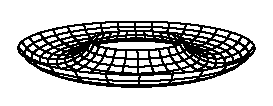
\includegraphics{asy/gutter}
\end{wrapfigure}

%%%%%%%%%%%%%%%%%%%%%%%%%%%%%%%%%%%%%%%%%%%%%%
\subsection*{Round gutter\hard}
\label{half-torus}

A round gutter is the surface shown on the picture.

}

More precisely, consider the torus $T$; a surface generated by revolving a circle in $\RR^3$ around an axis coplanar with the circle.
Let $\gamma\z\subset T$ be one of the circles in $T$ that locally separates positive and negative curvature on $T$;
a plane containing $\gamma$ is tangent to $T$ at all points of $\gamma$.
Then a neighborhood of $\gamma$ in $T$ is called 
\index{gutter}\emph{round gutter}
and the circle $\gamma$ is called its {}\emph{main latitude}.



\begin{pr}
Let $\Omega\subset \RR^3$ be a round gutter with main latitude $\gamma$. 
Assume that $\iota\:\Omega\z\to\RR^3$ 
is a smooth length-preserving embedding that is sufficiently close to the identity.
Show that $\gamma$ and $\iota(\gamma)$ are congruent;
that is, there is an isometric motion of $\RR^3$ sending $\gamma$ to $\iota(\gamma)$
\end{pr}



%%%%%%%%%%%%%%%%%%%%%%%%%%%%%%%%%%%%%%%%%%%%%%
\subsection*{Non-contractible geodesics}
\label{torus}

\begin{pr}
Give an example of a non-flat metric 
on the $2$-torus such that no closed geodesic is contractible.
\end{pr}


%%%%%%%%%%%%%%%%%%%%%%%%%%%%%%%%%%%%%%%%%%%%%%
\subsection*{Two disks}
\label{Two disks}

\begin{pr}
Let $\Sigma_1$ and $\Sigma_2$ be two smoothly embedded open disks in $\mathbb R^3$ 
that have a common closed smooth curve $\gamma$.
Show that there is a pair of points  $p_1\in \Sigma_1$ and $p_2\in \Sigma_2$ with parallel tangent planes.
\end{pr}



\section*{Semisolutions}
%%%%%%%%%%%%%%%%%%%%%%%%%%%%%%%%%%%%%%%%%%%%%%%%%%
\parbf{Involute of  geodesic.}
Let $W$ be the closed unbounded set formed by $\Sigma$ and its exterior points.
Choose $t\in (0,\ell)$;
denote by $\gamma_t$ the concatenation of the line segment $[p_t\gamma(t)]$ and the arc $\gamma|_{[t,\ell]}$.
The key step is to show the following:

\begin{cl}{$({*})$} The curve $\gamma_t$ is a minimizing geodesic in the intrinsic metric induced on $W$.
\end{cl}


Try to prove it before reading further.

\medskip

Let $\Pi_t$ be the tangent plane to $\Sigma$ at $\gamma(t)$.
Consider the curve $\alpha(t)=p_t$.
Note that  
$\alpha(t)\z\in\Pi_t$,
$\alpha'(t)\perp\Pi_t$
and $\alpha'(t)$ points to the side of $\Pi_t$ opposite to $\Sigma$.



It follows that for any $x\in\Sigma$ the function  
\[t\mapsto |x - p_t|
\quad\text{and, therefore,}\quad
t\mapsto |x - p_t|_W\] are non-decreasing;
here $|x - p_t|_W$ stays for the intrinsic distance from $x$ to $p_t$ in $W$.


\begin{wrapfigure}{r}{43 mm}
\vskip-6mm
\centering
\includegraphics{mppics/pic-205}
\end{wrapfigure}

On the other hand, by construction 
\[|q - p_t|_W\le |q - p|_\Sigma;\] 
therefore, from the above 
\[|q - p_t|_W= |q - p|_\Sigma\]
for any $t$.
Hence $(*)$ follows.

Now assume that $q$ is visible from $p_t$ for some $t$;
that is, the line segment $[qp_t]$ intersects $\Sigma$ only at $q$.
From the above, 
$\gamma_t$  coincides with the line segment $[qp_t]$.
On the other hand, $\gamma_t$ contains $\gamma(t)\in\Sigma$, a contradiction.\qeds

This problem is based on an observation used by Anatoliy Milka in the proof of his (beautiful) generalization of the comparison theorem for convex surfaces \cite{milka-geod}.

%%%%%%%%%%%%%%%%%%%%%%%%%%%%%%%%%%%%%%%%%%%%%%%%%%

\begin{wrapfigure}{r}{43 mm}
\vskip-0mm
\centering
\includegraphics{mppics/pic-206}
\end{wrapfigure}

\parbf{Simple geodesic.} 
Look at two combinatorial types of a self-intersection shown in the diagram.
One of them can and the other cannot appear as self-intersections of a geodesic on an unbounded convex surface.
Try to determine which is which before reading further.

\medskip

Let $\gamma$ be a two-sided infinite geodesic in $\Sigma$.
The following is the key statement in the proof.

\begin{cl}{$({*})$}
The geodesic $\gamma$ contains at most one simple loop.
\end{cl}

To prove $({*})$, we use the following observation.

\begin{cl}{$({*}{*})$}
The integral curvature $\omega$ of $\Sigma$ cannot exceed $2\cdot\pi$.
\end{cl}

Indeed, since $\Sigma$ is unbounded and convex,
it surrounds a half-line.
Consider a coordinate system with this half-line as the positive half of its $z$-axis. 
In these coordinates, the surface $\Sigma$ is described as a graph $z=f(x,y)$ of a convex function $f$.
In particular all outer normal vectors to $\Sigma$ have negative $z$-coordinate;
in other words they point to the south hemisphere.
Therefore the area of the spherical image of $\Sigma$ is at most $2\cdot\pi$.
The area of this image is the integral of the Gauss curvature over $\Sigma$. 
Hence $({*}{*})$ follows.

From the Gauss--Bonnet formula, we get the following conclusion.
If $\phi$ is the angle at the base of a simple geodesic loop then the integral curvature surrounded by the loop equals $\pi+\phi$. 
In particular $({*}{*})$ implies that $\phi\le\pi$; in other words, there are no \emph{concave loops}.

Now assume that $({*})$ does not hold, so that a geodesic has two simple loops.
Note that the disks bounded by the loops  have to overlap,
otherwise the curvature of $\Sigma$ would exceed $2\cdot\pi$.
But if they overlap, then it is easy to show that the curve also contains a concave loop, 
which contradicts the above observation.%
\footnote{This observation implies that the right picture on the above diagram cannot be realized by a geodesic.}

If a geodesic $\gamma$ has a self-intersection,
then it contains a simple loop.
From $({*})$, there is only one such loop;
it cuts a disk from $\Sigma$ 
and goes around it either clockwise or counterclockwise.
This way we divide all the self-intersecting geodesics 
into two sets which we will call {}\emph{clockwise} and {}\emph{counterclockwise}.

Note that the geodesic $t\mapsto \gamma(t)$ is clockwise 
if and only if 
$t\z\mapsto \gamma(-t)$
is counterclockwise.
The sets of clockwise and counterclockwise are open and the space of all geodesics is connected. 
It follows that there are geodesics 
which aren't clockwise nor counterclockwise.
Those geodesics have no self-intersections.\qeds

Note that the proof implies that a two-sided infinite geodesic can be found among geodesics containing a given point in $\Sigma$.

The problem is due to Stephan Cohn-Vossen \cite[see Satz 9 in][]{convossen};
generalizations were obtained  by 
Vladimir Streltsov and Alexandr Alexandrov 
\cite{streltsov-alexandrov} 
and 
by Victor Bangert \cite{bangert}.


%%%%%%%%%%%%%%%%%%%%%%%%%%%%%%%%%%%%%%%%%%%%%%%%%%
\parbf{Geodesics for birds.}
Choose a unit-speed geodesic in $W$, say
\[\gamma\:t\mapsto(x(t),y(t),z(t)).\]
We can assume that $\gamma$ is defined on a closed interval $[a,b]$.
The key step is to show the following:

\begin{cl}{$({*})$} 
The function $t\mapsto z$ is concave.
\end{cl}


Parametrize the plane curve $t\mapsto (x(t),y(t))$ by the arc length $s$
and reparametrize $\gamma$ by $s$.

\begin{wrapfigure}{r}{35 mm}
\vskip-4mm
\centering
\includegraphics{mppics/pic-208}
\end{wrapfigure}

Note that the function $s\mapsto z$ is concave.
Indeed, suppose $s\mapsto z$ is not concave around $s_0$.
Then one could shorten $\gamma$ by increasing its $z$ component in a small interval around $s_0$, while keeping its endpoints fixed.
After the deformation, the curve still lies in $W$.
The latter contradicts that $\gamma$ is locally length minimizing.

Finally note that concavity of $s\mapsto z$ is equivalent to the concavity of $t\mapsto z$.
Hence $({*})$ follows.



Since $f$ is smooth, 
the curve $\gamma(t)$ is $C^{1,1}$; 
that is, its first derivative $\gamma'(t)$ is a well defined Lipschitz function.
It follows that its second derivative $\gamma''(t)$ is defined almost everywhere.

Since $z(t)$ is concave, we have $z''(t)\le 0$.
Since $f$ is $\ell$-Lipschitz, $z(t)$ is $\tfrac{\ell}{\sqrt{1+\ell^2}}$-Lipschitz.
It follows that 
\[\int\limits_a^b |z''(t)|\le 2\cdot\tfrac{\ell}{\sqrt{1+\ell^2}}.\]

The curvature vector $\gamma''(t)$ is perpendicular to the surface.
Since the surface has slope at most $\ell$,
we get 
\[|\gamma''(t)|\le |z''(t)|\cdot\sqrt{1+\ell^2}.\]
Hence 
\[\int\limits_a^b |\gamma''(t)|\le 2\cdot\ell.\qedsin\]
\medskip

The statement holds for general $\ell$-Lischitz functions,
not necessarily smooth.
The given bound is optimal, the equality is attained by a two-side infinite geodesic on the graph of  
\[f(x,y)=-\ell\cdot\sqrt{x^2+y^2}.\]

The problem is due to David Berg \cite{berg},
the same bound for convex $\ell$-Lipschitz surfaces was proved earlier by Vladimir Usov \cite{usov}.
The observation $({*})$
is called \index{Liberman’s lemma}\emph{Liberman’s lemma}; 
it was used earlier 
to bound the total curvature
of a geodesic on a convex surface \cite{liberman}.\footnote{It is a part of the thesis of Joseph Liberman, defended a couple of months before his death in WWII.}
This lemma is often useful when working with geodesics on general convex surfaces.

%%%%%%%%%%%%%%%%%%%%%%%%%%%%%%%%%%%%%%%%%%%%%%%%%%
\parbf{Immersed surface.}
Let $\ell$ be a linear function that vanishes on $\Pi$ 
and is positive on $\Sigma$. 
We will apply a Morse type argument for the restriction of $\ell$ to $\Sigma$.

\medskip

Let $z_0$ be a maximum of $\ell$ on $\Sigma$;
set $s_0=\ell(z_0)$.
Given $s<s_0$, denote by $\Sigma_s$ the connected component of $z_0$ in $\Sigma\cap\ell^{-1}([s,s_0])$.
Note that for all $s$ sufficiently close to $s_0$
we have
\begin{itemize}
\item $\Sigma_s$ is an embedded disk;
\item $\partial\Sigma_s$ is a convex plane curve.
\end{itemize}

Consider the set $A\subset [0,s_0)$ such that for any $a\in A$ these two conditions hold for any $s\in [a,s_0)$.
Observe that $A$ is open and closed in $[0,s_0)$.
Whence $A=[0,s_0)$; in particular, these conditions hold for $s=0$.

Since $\Sigma$ is connected, $\Sigma_0=\Sigma$.
Hence the result follows.\qeds

This problem is discussed in the lectures of Mikhael Gromov \cite[see \S$\tfrac12$~in][]{gromov-SGMC}.

%%%%%%%%%%%%%%%%%%%%%%%%%%%%%%%%%%%%%%%%%%%%%%%%%%
\parbf{Periodic asymptote.}
Arguing by contradiction, assume that there is a geodesic $\gamma$ on the surface $\Sigma$ with a periodic asymptote $\delta$. 

Passing to a finite cover of $\Sigma$, we can ensure that the asymptote has no self-intersections.
In this case, 
the restriction $\gamma|_{[a,\infty)}$  
has no self-intersections 
if $a$ is sufficiently large.

Cut $\Sigma$ along $\gamma([a,\infty))$ and then cut from the obtained surface an infinite triangle $\triangle$. 
The triangle $\triangle$ has two sides formed by both sides of cuts along $\gamma$;
let us denote these sides of $\triangle$ by $\gamma_-$ and $\gamma_+$.
Note that 
\[\area\triangle<\area \Sigma<\infty\leqno(*)\]
and both sides $\gamma_\pm$ 
are infinite minimizing geodesics in $\triangle$.

Consider the Busemann function $f$ for $\gamma_+$ [defined on page~\pageref{page:Busemann function}];
denote by $\ell(t)$ the length of the level curve $f^{-1}(t)$.
Let $-\kappa(t)$  be the total curvature of the sup-level set $f^{-1}([t,\infty))$.  
From the Gauss--Bonnet formula,
\[\ell'(t)=\kappa(t).\leqno({*}{*})\]

The level curve $f^{-1}(t)$ can be parametrized by a unit-speed curve, say $\theta_t\:[0,\ell(t)]\to \triangle$.
By the coarea formula we have
\[\kappa'(t)
=
-\int\limits_0^{\ell(t)} K_{\theta_t(\tau)}\cdot d\tau,
\]
where $K_x$ denotes the Gauss curvature of $\Sigma$ at the point $x$.
Since $K_{\theta_t(0)}\z=K_{\theta_t(\ell_t)}=0$ and the surface is smooth,
there is a constant $C$ such that $|K_{\theta_t(\tau)}|\le C\cdot \ell(t)^2$ for all $t$, $\tau$.
Therefore
\[\kappa'(t)\le C\cdot \ell(t)^3 \leqno(\asterism)\]

Together, $({*}{*})$ and $(\asterism)$ imply that there is $\eps>0$ such that
\[\ell(t)\ge \frac\eps{t-a}\]
for sufficiently large $t$.
By the coarea formula we get 
\[\area\triangle=\int\limits_a^\infty\ell(t)=\infty;\]
the latter contradicts $(*)$.\qeds

I learned the problem from 
Dmitri Burago 
and Sergei Ivanov, 
it originated from a discussion with
Keith Burns, 
Michael Brin 
and Yakov Pesin.

Here is a motivation.
Let $\Sigma$ be a closed surface with non-positive curvature that is not flat.
The space $\Gamma$ of all unit-speed geodesics $\gamma\:\RR\z\to\Sigma$ can be identified with the unit tangent bundle $\UU\Sigma$. 
In particular $\Gamma$ comes with a natural choice of measure.
Denote by $\Gamma_0\subset \Gamma$ the set of geodesics that run in the set of zero curvature all the time.
It is expected that $\Gamma_0$ has vanishing measure.
In all known examples $\Gamma_0$ contains only periodic geodesics in only finitely many homotopy classes \cite[see also][]{hertz}.

%%%%%%%%%%%%%%%%%%%%%%%%%%%%%%%%%%%%%%%%%%%%%%%%%%
\parbf{Saddle surface.}
Denote by $\Sigma^\circ$ the interior of $\Sigma$.
Choose a plane $\Pi$. 
Note that the intersection $\Pi\cap \Sigma^\circ$ 
locally looks either like a curve or like two curves intersecting transversally;
in the latter case $\Pi$ is tangent to $\Sigma^\circ$ at the intersection point.

Further note that $\Pi\cap \Sigma^\circ$ has no cycle.
Otherwise $\Sigma$ would fail to be saddle at the point of the disk surrounded by that cycle maximizing the distance to $\Pi$.

If $\Sigma$ is not a graph then there is a point $p\in\Sigma$ with a vertical tangent plane;
denote this plane by $\Pi$.
The intersection $\Pi\cap\Sigma$ has cross-point at~$p$.

Since the boundary of $\Sigma$ projects injectively to a closed convex curve in $(x,y)$-plane,
the intersection of $\Pi\cap\partial \Sigma$ has at most 2 points --- these are the only endpoints of $\Pi\cap\Sigma$.

It follows that the connected component of $p$ in $\Pi\cap\Sigma$ is a tree 
with a vertex of degree 4 at $p$ and at most two end-points, a contradiction.\qeds

The described idea can be used to prove the result of Richard Schoen and Shing-Tung  Yau \cite{schoen-yau-2D} which gives a sufficient condition for a harmonic map between surfaces to be a diffeomorphism.
Unlike the original proof, it requires no calculations.

The proof above is based on the observation 
that for any saddle surface $\Sigma$ and plane $\Pi$,
each connected component of $\Sigma\backslash \Pi$ is either unbounded or intersects the boundary curve.
This observation plays a central role in the proof of Sergei Bernstein \cite{bernshtein}
of the following problem:

\begin{pr}
Show that a smooth bounded function $f\:\RR^2\to\RR$ cannot have a strictly saddle graph.
\end{pr}

One could go further and define a \emph{generalized saddle surface} as an arbitrary (non necessarily smooth) surface satisfying the observation above.
The geometry of these surfaces is far from being understood,
Samuil Shefel has a number of beautiful results about them, 
\cite[see][and the references therein]{shefel, AKP-invitation}.
The statement of the problem holds for these generalized saddle surfaces, but
the proof is tricky \cite{petrunin-stadler}.


%%%%%%%%%%%%%%%%%%%%%%%%%%%%%%%%%%%%%%%%%%%%%%%%%%
\parbf{Asymptotic line.}
Denote by $\Pi_t$ the tangent plane to $\Sigma$ at $\gamma(t)$ and by $\ell_t$ the tangent line of $\gamma$ at time $t$.

Since $\gamma$ is asymptotic, the plane $\Pi_t$ rotates around $\ell_t$ as $t$ changes.
Since $\Sigma$ is saddle, the speed of rotation cannot vanish.%
\footnote{By the Beltrami--Enneper theorem, if $\gamma$ has unit speed, then the speed of rotation is $\pm\sqrt{-K}$, where $K$ is the Gauss curvature which cannot vanish on a saddle surface.}

Note that $\Pi_t$ is a graph of a linear function, say $h_t$, defined on the $(x, y)$-plane.
Denote by $\bar\ell_t$ the projection of $\ell_t$ to the $(x, y)$-plane.
The described rotation of $\Pi_t$ can be expressed algebraically:
the derivative $\tfrac{d}{dt}h_t(w)$ vanishes at the point $w$ if and only if $w\in \bar\ell_t$ 
and the derivative changes sign if $w$ changes the side of $\bar\ell_t$.

Denote by $\bar\gamma$ the projection of $\gamma$ to the $(x, y)$-plane.
If $\bar\gamma$ is star shaped with respect to a point $w$, then $w$ cannot cross $\bar\gamma_t$.
Therefore the function $t\mapsto h_t(w)$ is monotone on $\SSS^1$.
Observing that this function cannot be constant, we arrive at a contradiction.\qeds

The problem is discussed by Dmitri Panov \cite{panov-curves}.

%%%%%%%%%%%%%%%%%%%%%%%%%%%%%%%%%%%%%%%%%%%%%%%%%%
\parbf{Minimal surface.}
Without loss of generality we may assume that the sphere is centered at the origin of $\RR^3$.

Let $h$ be the restriction of the function $x\mapsto \tfrac12\cdot|x|^2$ to the surface $\Sigma$.
Direct calculations show that $\Delta_\Sigma h =  2$;
here $\Delta_\Sigma$ denoted Laplacian on $\Sigma$.
Applying the divergence theorem for the gradient $\nabla_\Sigma h$
in $\Sigma_r\z=\Sigma\cap B(0,r)$, we get
\[2\cdot \area\Sigma_r\le r\cdot\length [\partial\Sigma_r].\]

Set $a(r)=\area\Sigma_r$.
By the coarea formula, $a'(r)\ge\length [\partial\Sigma_r]$ for almost all $r$.
Therefore the function
\[f\:r\mapsto \frac{\area\Sigma_r}{r^2}
\]
is non-decreasing in the interval $(0,1)$.

Since $f(r)\to \pi$ as $r\to0$, the result follows.\qeds

We described a partial case of the so-called \index{monotonicity formula}\emph{monotonicity formula} for minimal surfaces.

The same argument shows that if $0$ is a double point
of $\Sigma$ then $\area\Sigma\z\ge 2\cdot \pi$.
This observation was used to prove 
that the minimal disk bounded by a simple closed curve with total curvature $\le 4\cdot\pi$ 
is necessarily embedded.
It was proved by 
Tobias Ekholm, 
Brian White 
and Daniel Wienholtz
\cite{EWW};
an amusing variation of this proof
was obtained by 
Stephan Stadler \cite{stadler-FM}.
This result also implies that any embedded circle of total curvature at most $4\cdot\pi$ is unknot.
The latter was proved independently by Istv{\'a}n F{\'a}ry \cite{fary-knot} and  John Milnor \cite{milnor}.

Note that if we assume in addition that the surface is a disk,
then the statement holds for any saddle surface. 
Indeed, denote by $S_r$ the sphere of radius $r$ concentrical with the unit sphere. 
Then according to the problem ``A curve on a sphere'' [page \pageref{A curve in a sphere}], 
\[\length[\partial\Sigma_r]\ge 2\cdot\pi\cdot r.\]
Then by the coarea formula we get $\area\Sigma\ge \pi$.

On the other hand, there are saddle surfaces homeomorphic to the cylinder
having an arbitrarily small area in the ball. 

If $\Sigma$ does not pass thru the center 
and we only know the distance, say $r$, 
from the center to $\Sigma$,
then the optimal bound is $\pi\cdot(1-r^2)$.
This question was open for about 40 years and proved by Simon Brendle and Pei-Ken Hung \cite{brende-hung};
their proof is based on a similar idea and is quite elementary.
Earlier Herbert Alexander, 
David Hoffman
and Robert Osserman 
proved it for two cases: (1) for disks and (2) for arbitrary area minimizing surfaces, any dimension and codimension
 \cite{alexander-osserman,alexander-hoffman-osserman}.






%%%%%%%%%%%%%%%%%%%%%%%%%%%%%%%%%%%%%%%%%%%%%%%%%%
\parbf{Round gutter.}
Without loss of generality, we can assume that the length of $\gamma$ is $2{\cdot}\pi$ and its intrinsic curvature is $1$ at all points.

Let $K$ be the convex hull of $\hat\Omega=\iota(\Omega)$.
Part of $\hat\Omega$ touches the boundary of $K$ and the rest lies in the interior of $K$. 
Denote by $\hat\gamma$ the curve in $\hat\Omega$ dividing these two parts.

First note that the Gauss curvature of $\hat\Omega$ should vanish at the points of $\hat\gamma$;
in other words, $\hat\gamma=\iota(\gamma)$.
Indeed, since $\hat\gamma$ lies on the convex part, 
the Gauss curvature at the points of $\hat\gamma$ should be non-negative. 
On the other hand, $\hat\gamma$ bounds a flat disk in $\partial K$;
therefore its integral intrinsic curvature should be $2{\cdot}\pi$.
If the Gauss curvature is positive at some point of $\hat\gamma$, 
then by the Gauss--Bonnet formula, the total intrinsic curvature of $\hat\gamma$ should be smaller than $2{\cdot}\pi$, a contradiction.

On the other hand, $\hat\gamma$ is an asymptotic line.
Indeed, if the direction of $\hat\gamma$ is not asymptotic at some $t_0$,
then $\hat\gamma(t_0 \pm\eps)$ lies the interior of $K$ for some small $\eps>0$, a contradiction.

Therefore, as the space curve,
$\hat\gamma$ has to be a closed curve with constant curvature $1$.
Any such curve is congruent to a unit circle.\qeds

It is not known whether $\hat\Omega$ is congruent to $\Omega$ or not.

The solution presented above is based on my answer 
to the question of Joseph O'Rourke \cite{rourke}.
Here are some related statements.
\begin{itemize}
\item A gutter is second order rigid;
this was proved by Eduard Rembs
[see \ncite{rembs} and also page 135 in \ncite{efimov}].
\item Any second order rigid surface does not admit analytic deformation 
[proved by Nikolay Efimov; page 121 in \ncite{efimov}]
and for the surfaces of revolution, the assumption of analyticity can be removed 
\cite[proved by Idzhad Sabitov, see][]{sabitov}.
\end{itemize}









%%%%%%%%%%%%%%%%%%%%%%%%%%%%%%%%%%%%%%%%%%%%%%%%%%
\parbf{Non-contractible geodesics.}
A torus of revolution is an example.

Indeed, it has a family of {}\emph{meridians} --- a family of circles that form closed geodesics.
Note that a geodesic on the torus is either a meridian
or it intersects meridians transversally.
In the latter case all the meridians are crossed by the geodesic in the same direction.

Note that a contractible curve has to cross each meridian an equal number of times in both directions.
Therefore no geodesic of the torus is contractible.\qeds 


I learned this problem 
from the book of Mikhael Gromov \cite{gromov-MetStr},
where it is attributed to Y. Colin de Verdi\`ere.
The same argument can be used to show that a torus with a geodesic foliation has no contractible closed geodesics.
I do not know other examples of that type \cite{petrunin-torus}; namely the following question is open:

\begin{pr}
Are there examples of Riemannian metrics on the 2-torus without closed null-homotopic geodesics and without a geodesic foliation?
\end{pr}


%%%%%%%%%%%%%%%%%%%%%%%%%%%%%%%%%%%%%%%%%%%%%%%%%%
%%%%%%%%%%%%%%%%%%%%%%%%%%%%%%%%%%%%%%%%%%%%%%%%%%
\parbf{Two disks.}
Choose a continuous map $h\:\Sigma_1\to \Sigma_2$
that is the identity on $\gamma$.
Let us prove that for some $p_1\in \Sigma_1$ and $p_2=h(p_1)\in \Sigma_2$,
the tangent planes $\T_{p_1} \Sigma_1$ and  $\T_{p_2} \Sigma_2$ are parallel;
this fact is stronger than the one required.

\medskip

Arguing by contradiction,
assume that such a point does not exist.
Then for each $p\in\Sigma_1$
there is a unique line $\ell_p\ni p$ 
 parallel to both $\T_{p} \Sigma_1$ and $\T_{h(p)} \Sigma_2$.

Note that the lines $\ell_p$ form a tangent line distribution over $\Sigma_1$
and $\ell_p$ is tangent to $\gamma$ at all $p\in\gamma$.

Let $\Delta$ be the disk in $\Sigma_1$ bounded by $\gamma$.
Consider the doubling of $\Delta$ along  $\gamma$;
it is diffeomorphic to $\mathbb S^2$.
The line distribution $\ell$ lifts to a line distribution on the doubling.
The latter contradicts the hairy ball theorem.\qeds


This proof was suggested nearly simultaneously 
by Steven Sivek 
and Damiano Testa \cite{two-disks}.

Note that the same proof works when $\Sigma_i$ are oriented open surfaces and $\gamma$ cuts a compact domain in each $\Sigma_i$.

There are examples of three disks $\Sigma_1$, $\Sigma_2$ and $\Sigma_3$
with a common closed curve $\gamma$ such that there is
no triple of points $p_i\in\Sigma_i$ with parallel tangent planes.
Such examples can be found among ruled surfaces \cite{three-disks}.

\csname @openrightfalse\endcsname
\chapter{Comparison geometry}

In this chapter we consider Riemannian manifolds with curvature bounds.

This chapter is very demanding;
we assume that the reader is familiar with   
shape operator and second fundamental form, 
equations of Riccati and Jacobi,
comparison theorems,
and Morse theory.
The classical book \cite{cheeger-ebin} covers all the  necessary  material.

%%%%%%%%%%%%%%%%%%%%%%%%%%%%%%%%%%%%%%%%%
\subsection*{Geodesic immersion\hard}
\label{Geodesic immersion}

An isometric immesion $\iota\:N\looparrowright M$ from one Riemannian manifold to another is called \index{totally geodesic}\emph{totally geodesic} if it maps any geodesic in $N$ to a geodesic in $M$.

\begin{pr}
Let $M$ and $N$ be simply connected positively curved Riemannian manifolds and $\iota\:N\looparrowright M$ a totally geodesic immersion.
Assume that 
\[\dim N>\tfrac 12\cdot \dim M.\]
Prove that $\iota$ is an embedding.
\end{pr}

%%%%%%%%%%%%%%%%%%%%%%%%%%%%%%%%%%%%%%%%%%%%%%%%%%
\parit{Semisolution.}
Set $n=\dim N$, $m=\dim M$.

Choose a smooth increasing strictly concave function $\phi$.
Consider the function $f=\phi\circ\dist_N$,
where $\dist_N(x)$ denotes the distance from $x\in M$ to $N$.

Note that if $f$ is smooth at some point $x\in M$ 
then the Hessian of $f$ at $x$ (briefly $\Hess_xf$)
has at least $n+1$ negative eigenvalues.

Moreover, at any point $x\notin \iota(N)$ the same holds in the barrier sense\label{page:barrier sense}.
That is, there is a smooth function $h$ defined on $M$
such that $h(x)=f(x)$, $h(y)\ge f(y)$ for any $y$
and $\Hess_xh$ has at least $n+1$ negative eigenvalues.

Use that $m< 2\cdot n$ and the described property to prove the following
analog of Morse lemma for $f$.

\begin{cl}{$({*})$}
 Given $x\notin \iota(N)$ there is a neighborhood $U\ni x$ such that the set 
\[U_-=\set{z\in U}{f(z)<f(x)}\] is simply connected.
\end{cl}

Since $M$ is simply connected,
any closed curve in $\iota(N)$
can be contracted by a disc, say $s_0\:\mathbb D\to M$.

Applying the claim $({*})$, one can construct an $f$-decreasing homotopy $s_t$ that starts at $s_0$ and ends in $\iota(N)$;
that is, there is 
a homotopy $s_t\:\mathbb D\z\to M$, $t\in [0,1]$ 
such that $s_t(\partial \mathbb D)\subset \iota(N)$ for any $t$ 
and $s_1(\mathbb D)\subset \iota(N)$.
It follows that $\iota(N)$ is simply connected.

Finally assume that $a$ and $b$ are distinct points in $N$ such that $\iota(a)=\iota(b)$.
If $\gamma$ is a path from $a$ to $b$ in $N$ then the loop $\iota\circ\gamma$ is not contractible in $\iota(N)$.
Therefore if $\iota\:N\to M$ has a self-intersection,
then the image
$\iota(N)$ is not simply connected.
Hence the result follows.\qeds


The statement was proved by 
Fuquan Fang, 
S\'ergio Mendon\c{c}a 
and Xiaochun Rong \cite{FMR}.
The main idea was discovered by 
Burkhard Wilking \cite{wilking-2003}.

%%%%%%%%%%%%%%%%%%%%%%%%%%%%%%%%%%%%%%%%%
\subsection*{Geodesic hypersurface}
\label{Geodesic hypersurface}

The totally geodesic embedding is defined before the previous problem.

\begin{pr}
Assume a compact connected positively curved manifold $M$ has a totally geodesic embedded hypersurface.
Show that either $M$ or its double covering is homeomorphic to the sphere.
\end{pr}

%%%%%%%%%%%%%%%%%%%%%%%%%%%%%%%%%%%%%%%%%
\subsection*{If convex, then embedded}
\label{If convex then embedded} 

\begin{pr}
Let $M$ be a complete simply connected Riemannian manifold 
with non-positive curvature 
and dimension at least $3$.
Prove that any immersed locally convex
compact hypersurface $\Sigma$ in $M$ is embedded.
\end{pr}

Let us summarize some statements about complete simply connected Riemannian manifolds 
with non-positive curvature.

By the Cartan--Hadamard theorem, for any point $p\in M$
the exponential map $\exp_p\:\T_p\to M$ is a diffeomorphism.
In particular, $M$ is diffeomorphic to the Euclidean space of the same dimension.
Moreover, any geodesic in $M$ is minimizing,
and any two points in $M$ are connected by a unique minimizing geodesic,

Further, $M$ is a $\CAT(0)$ space; that is, it satisfies a global angle comparison which we are about to describe.
Let $[xyz]$ be a triangle in $M$;
that is, $[xyz]$ is formed by three distinct points $x,y,z$ pairwise connected by geodesics.
Consider its model triangle $[\tilde x\tilde y\tilde z]$ in the Euclidean plane;
that is, $[\tilde x\tilde y\tilde z]$ has the same side lengths as $[xyz]$.
Then each angle in $[xyz]$ cannot exceed the corresponding angle in $[\tilde x\tilde y\tilde z]$.
This inequality can be written as
\[\tilde\measuredangle(y\,^x_z)\ge\measuredangle\hinge yxz,\]
where $\measuredangle\hinge yxz$ denotes the angle of the hinge $\hinge yxz$ formed by two geodesics $[yx]$ and $[yz]$ 
and $\tilde\measuredangle(y\,^x_z)$ denotes the corresponding angle in the model triangle $[\tilde x\tilde y\tilde z]$.

From this comparison it follows that any connected closed locally convex sets in $M$ is globally convex.
In particular, if $\Sigma$ is embedded then it bounds a convex set.


%%%%%%%%%%%%%%%%%%%%%%%%%%%%%%%%%%%%%%%%%
\subsection*{Immersed ball\hard}
\label{Immersed ball}

\begin{pr}
Prove that any immersed locally convex
hypersurface $\iota\:\Sigma\looparrowright M$
in a compact positively curved manifold $M$ of dimension $m\ge 3$ is the boundary of an immersed ball. 
That is, there is an immersion of a closed ball $f\:\bar B^m\looparrowright M$ and a diffeomorphism $h\:\Sigma\to\partial \bar B^m$
such that $\iota=f\circ h$.
\end{pr}

%%%%%%%%%%%%%%%%%%%%%%%%%%%%%%%%%%%%%%%%%
\subsection*{Minimal surface in the sphere}
\label{minimal surface}\label{almgren} 

A  smooth $n$-dimensional surface $\Sigma$ in
an $m$-dimensional Riemannian manifold $M$ is called \index{minimal surface}\emph{minimal}
if it locally minimizes the $n$-dimensional area;
that is, sufficiently small regions of $\Sigma$ do not admit area decreasing deformations with fixed boundary.

The minimal surfaces can be also defined via mean curvature vector as follows.
Let $\T=\T\,\Sigma$ and $\mathrm{N}=\mathrm{N}\,\Sigma$ denote the tangent and the normal bundle correspondingly.
Let $s$ denotes the second fundamental form of $\Sigma$;
it is a quadratic from on $\T$ with values in $\mathrm{N}$,
see the remark after problem ``Hypercurve'' below. 
Given an orthonormal basis $(e_i)$ in $\T_x$ set 
$$H_x=\sum_i s(e_i,e_i).$$
The vector $H_x$ lies in the normal space $\mathrm{N}_x$
and does not depend on the choice of orthonormal basis $(e_i)$.
This vector $H_x$ is called the mean curvature vector at $x\in \Sigma$. 

We say that $\Sigma$ is \index{minimal surface}\emph{minimal} if $H\equiv 0$.

\begin{pr}
Let $\Sigma$ be a closed $n$-dimensional 
minimal surface
in the unit $m$-dimensional sphere $\mathbb{S}^m$.
Prove that
$\vol_n \Sigma\ge \vol_n \mathbb{S}^n$.
\end{pr}

%%%%%%%%%%%%%%%%%%%%%%%%%%%%%%%%%%%%%%%%%
\subsection*{Hypercurve}
\label{codim=2}

The Riemann curvature tensor $R$
can be viewed as an operator $\text{\bf R}$ on the space of tangent bi-vectors $\bigwedge^2 \T$;
it is uniquely defined by the identity
$$\langle\mathbf{R}(X\wedge Y),V\wedge W\rangle
=
\langle R(X,Y)V,W\rangle.$$
The operator $\mathbf{R}\:\bigwedge^2 \T\to \bigwedge^2 \T$ is called the \index{curvature operator}\emph{curvature operator} and it is said to be {}\emph{positive definite} if
$\langle\mathbf{R}(\phi),\phi\rangle>0$ for all nonzero
bi-vector $\phi\in\bigwedge^2 \T$.


\begin{pr}
Let $M^m\hookrightarrow \RR^{m+2}$ be a closed smooth $m$-dimensional
submanifold and let  $g$ be the  induced Riemannian metric on $M^m$.
Assume that sectional curvature of $g$ is positive.
Prove that the curvature operator of $g$ is positive definite.
\end{pr}

The second fundamental form for manifolds of arbitrary codimension which we are about to describe might help to solve this problem.

Let $M$ be a smooth submanifold in $\RR^m$.
Given a point $p\in M$ denote by $\T_p$ and $\mathrm{N}_p=\T_p^\bot$
the tangent and normal space of $M$ at $p$.
The \index{second fundamental form}\emph{second fundamental form}\label{page:second fundamental form} of $M$ at $p$ is defined by 
\[s(X,Y)=(\nabla_X Y)^\bot,\]
where $(\nabla_X Y)^\bot$ a denotes the orthogonal projection of covariant derivative $\nabla_X Y$ onto the normal bundle.

The curvature tensor of $M$ can be found from the second fundamental form using the following  formula
\[\langle R(X,Y)V,W\rangle=\langle s(X,W),s(Y,V)\rangle-\langle s(X,V),s(Y,W)\rangle,\]
which is a direct generalization of the formula for Gauss curvature of a surface.


%%%%%%%%%%%%%%%%%%%%%%%%%%%%%%%%%%%%%%%%%
\subsection*{Horo-sphere}
\label{Horosphere}

We say that a Riemannian manifold has negatively pinched sectional curvature if its sectional curvatures at all points in all sectional directions lie in an interval $[-a^2, -b^2]$, for fixed constants $a>b>0$.

Let $M$ be a complete Riemannian manifold
and $\gamma$ a ray in $M$; 
that is, $\gamma\:[0, \infty)\to M$ is a minimizing unit-speed geodesic.

The \label{page:Busemann function}\index{Busemann function}\emph{Busemann function} $\bus_\gamma\:M\to\RR$ is defined by
$$\bus_\gamma(p)=\lim_{t\to\infty}\left(|p-\gamma(t)|_M-t\right).$$
From the triangle inequality, 
the expression under the limit is non-increasing in $t$; 
therefore  the limit above is defined for any $p$.

A \index{horo-sphere}\emph{horo-sphere} in $M$ is defined as a level set of a Busemann function
on $M$.

We say that a complete Riemannian manifold $M$ has \index{polynomial volume growth}\emph{polynomial volume growth} if for some (and therefore any) $p\in M$ we have 
$$\vol B(p,r)_M\z\le C\cdot (r^k+1),$$ 
where $B(p,r)_M$ denotes the ball in $M$ and  $C$, $k$ are constants.

\begin{pr} Let $M$ be a complete simply connected manifold with negatively pinched sectional curvature
and $\Sigma\subset M$ an horo-sphere in $M$.
Show that
$\Sigma$ with the induced intrinsic metric 
has polynomial volume growth.
\end{pr}

%%%%%%%%%%%%%%%%%%%%%%%%%%%%%%%%%%%%%%%%%
\subsection*{Number of conjugate points}
\label{Number of conjugate points}

Recall that points $p$ and $q$ on a geodesic $\gamma$ are called \index{conjugate points}\emph{conjugate} if there exists a non-zero Jacobi field along $\gamma$ that vanishes at $p$ and $q$. 

\begin{pr}
Let $s\:N\to M$ be a Riemannian submersion.
Suppose $N$ has nonpositive sectional curvature.
Show that any point $p$ in $M$ has at most $k=\dim N-\dim M$ conjugate points on any geodesic $\gamma\ni p$.
\end{pr}

%%%%%%%%%%%%%%%%%%%%%%%%%%%%%%%%%%%%%%%%%
\subsection*{Minimal spheres}
\label{Minimal spheres}

Recall that two subsets $A$ and $B$ in a metric space $X$ are called \index{equidistant sets}\emph{equidistant} if the distance function $\dist_A\:X\to\RR$ is constant on $B$ and $\dist_B$ is constant on $A$.

The minimal surfaces are defined on page \pageref{minimal surface}.

\begin{pr}
Show that a 
$4$-dimensional
compact 
positively curved 
Riemannian manifold 
cannot contain infinite number of  mutually
 equidistant minimal 2-spheres.
\end{pr}


%%%%%%%%%%%%%%%%%%%%%%%%%%%%%%%%%%%%%%%%%
\subsection*{Positive curvature and symmetry\thm}
\label{kleiner-hopf} 

\begin{pr}
Assume that $\mathbb S^1$ acts isometrically on a closed $4$-dimensional Riemannian manifold with positive sectional curvature.
Show that the action 
has at most $3$ isolated fixed points.
\end{pr}

The following statement might be useful.
If $(M,g)$ is a Riemannian manifold with sectional curvature $\ge \kappa$ that admits a continuous isometric action of a compact group $G$, 
then the quotient space $A=(M,g)/G$ is an Alexandrov space with curvature $\ge \kappa$;
that is, the conclusion of the Toponogov comparison theorem holds in $A$. 

For more on Alexandrov geometry see \cite{akp}.

%%%%%%%%%%%%%%%%%%%%%%%%%%%%%%%%%%%%%%%%%
\subsection*{Energy minimizer}
\label{Energy minimizer}

Let $F$ be a smooth map from a closed Riemannian manifold $M$ to a Riemannian manifold $N$.
The energy functional of $F$ is defined by
\[E(F)=\int\limits_M |d_xF|^2\cdot d_x\vol_M.\]
We assume that  
\[|d_xF|^2=\sum_{i,j}a_{i,j}^2,\]
where $(a_{i,j})$ denote the components 
of the differential $d_xF$ 
written in the orthonormal bases of the tangent spaces $\T_xM$ and $\T_{F(x)}N$.

\begin{pr}
Show that the identity map on $\RP^m$ is 
energy
minimizing in its homotopy class.
Here we assume that $\RP^m$ is equipped with the canonical metric.
\end{pr}


%%%%%%%%%%%%%%%%%%%%%%%%%%%%%%%%%%%%%%%%%
\subsection*{Curvature against injectivity radius\thm}
\label{scalar-curv}

\begin{pr} 
Let $(M,g)$ be a closed 
Riemannian $m$-dimensional manifold.
Assume average of sectional curvatures over all sectional directions of $(M,g)$ is $1$. 
Show that the injectivity radius of $(M,g)$ is at most $\pi$.
\end{pr}

Solutions of this and the previous problem use the fact that geodesic flow on the tangent bundle to a Riemannian manifold preserves the volume form; this is a corollary of Liouville's theorem about phase volume.

%%%%%%%%%%%%%%%%%%%%%%%%%%%%%%%%%%%%%%%%%
\subsection*{Approximation of a quotient}

\begin{pr}
Let $(M,g)$ be a compact Riemannian manifold 
and $G$ a compact Lie group acting by isometries on $(M,g)$.
Construct a sequence of metrics $g_n$ on a fixed manifold $N$ such that $(N,g_n)$ converges to the quotient space $(M,g)/G$ in the sense of Gromov--Hausdorff.
\end{pr}


%%%%%%%%%%%%%%%%%%%%%%%%%%%%%%%%%%%%%%%%%
\subsection*{Polar points\many}
\label{milka-polar} 

\begin{pr}
Let $M$ be a compact Riemannian manifold with sectional curvature at least $1$ 
and dimension at least $2$. 
Prove that for any point $p\in M$ there is a point $p^*\in M$ such that 
\[|p-x|_M+|x-p^*|_M\le \pi\]
for any $x\in M$.
\end{pr}

%%%%%%%%%%%%%%%%%%%%%%%%%%%%%%%%%%%%%%%%%
\subsection*{Isometric section\hard}
\label{Isometric section}

\begin{pr}
Let $M$ and $W$ be compact Riemannian manifolds,
$\dim W>\dim M$,
and $s\:W\to M$ a Riemannian submersion.
Assume that $W$ has positive sectional curvature.
Show that $s$ does not admit an isometric section;
that is, there is no isometric embedding $\iota\:M\hookrightarrow W$ such that $s\circ\iota(p)=p$ for any $p\in M$.
\end{pr}

%%%%%%%%%%%%%%%%%%%%%%%%%%%%%%%%%%%%%%%%%
\subsection*{Warped product}
\label{Warped product}
\label{page:warped product}

Let $(M,g)$ and $(N,h)$ be Riemannian manifolds 
and $f$ a smooth positive function defined on $M$.
Consider the product manifold $W\z=M\times N$.
Given a tangent vector 
$X\z\in \T_{(p,q)} W
\z=\T_p M\times \T_p N$ denote by 
$X_M\z\in \T M$ and $X_N\z\in \T N$ its projections.
Let us equip $W$ with the Riemannian metric defined by
\[s(X,Y)=g(X_M,Y_M)+f^2\cdot h(X_N,Y_N).\]
The obtained Riemannian manifold $(W,s)$ is called \index{warped product}\emph{warped product} of $M$ and $N$ with respect to $f\:M\to \RR$;
it can be written as  
\[(W,g)\z=(N,h)\times_f(M,g).\]

\begin{pr}
Let $M$ be an oriented 3-dimensional Riemannian manifold with positive scalar curvature 
and $\Sigma\subset M$ an oriented smooth hypersurface that is area minimizing in its homology class.

Show that there is a positive smooth function $f\:\Sigma\to \RR$
such that the warped product $\mathbb S^1\times_f \Sigma$
has positive scalar curvature;
here $\Sigma$ is equipped with the Riemannian metric
induced from $M$.
\end{pr}

%%%%%%%%%%%%%%%%%%%%%%%%%%%%%%%%%%%%%%%%%
\subsection*{No approximation\many}
\label{No approximation}

\begin{pr}
Prove that 
if $p\not=2$,
then $\RR^m$ 
equipped with the metric induced by the $\ell^p$-norm 
cannot be a
Gromov--Hausdorff limit of
$m$-dimensional Riemannian manifolds $(M_n,g_n)$ with $\Ric_{g_n}\z\ge C$ for some constant $C$.
\end{pr}

%%%%%%%%%%%%%%%%%%%%%%%%%%%%%%%%%%%%%%%%%
\subsection*{Area of spheres}
\label{Area of spheres}

\begin{pr}
Let $M$ be a complete non-compact Riemannian manifold 
with non-negative Ricci curvature and $p\in M$.
Show that there is $\eps>0$ such that 
$$\area\left[\partial B(p,r)\right]>\eps$$
for all sufficiently large $r$.
\end{pr}

%%%%%%%%%%%%%%%%%%%%%%%%%%%%%%%%%%%%%%%%%
\subsection*{Flat coordinate planes}
\label{Flat coordinate planes}

\begin{pr}
Let $g$ be a complete Riemannian metric on $\RR^3$ such that the coordinate planes $x=0$, $y=0$ and $z=0$ are flat and totally geodesic.
Assume the sectional curvature of $g$ is either non-negative or non-positive.
Show that in both cases $g$ is flat. 
\end{pr}

%%%%%%%%%%%%%%%%%%%%%%%%%%%%%%%%%%%%%%%%%
\subsection*{Two-convexity\many}
\label{Two-convexity}

An open subset $V$ with smooth boundary in the Euclidean space  
is called \index{two-convex set}\emph{two-convex} if at most one principle curvatures in the outward direction to $V$ is negative.

The two-convexity of $V$ is equivalent to the following property.
For any plane $\Pi$ and any closed curve $\gamma$ in the intersection  $V\cap \Pi$,
if $\gamma$ is contactable in $V$ then it is contactable in $\Pi\cap V$.

\begin{pr}
Let $K$ be a closed set bounded by a smooth surface
in $\RR^4$.
Assume that $K$ contains two coordinate planes 
$$\{(x,y,0,0)\in\RR^4\}
\quad
\text{and}
\quad
\{(0,0,z,t)\in\RR^4\}$$
in its interior 
and also belongs to the closed $1$-neighborhood of these two planes.

Show that the complement to $K$ is not two-convex.
\end{pr}


%%%%%%%%%%%%%%%%%%%%%%%%%%%%%%%%%%%%%%%%%???
\subsection*{Convex lens\thm}
\label{Convex lens}

\begin{pr} Let $D$ and $D'$ be two smooth discs with common boundary that bound a convex set (a lens) $L$ in a positively curved 3-dimensional Riemannian manifold $M$.
Assume that the discs meet at a small angle.
Show that the integral 
\[\int\limits_{D}k_1\cdot k_2\]
is small; here $k_1$ and $k_2$ denote the principle curvatures of $D$.
\end{pr}

The expected solution use the following relative version of the Bochner formula.
Let $M$ be a Riemannian manifold with boundary $\partial M$.
If $f\:M\to \RR$ is a smooth function that vanish on $\partial M$,
then 
\[\int\limits_M |\Delta f|^2
-|\Hess f|^2
-\langle\mathrm{Ric}(\nabla f),\nabla f\rangle
=\int\limits_{\partial M}
H\cdot|\nabla f|^2.\]
Here we denote by $\Ric$ the Ricci curvature of $M$ 
and by $H$ the mean curvature of $\partial M$, we assume that $H\ge 0$ is the boundary is convex.
%???REF



%%%%%%%%%%%%%%%%%%%%%%%%%%%%%%%%%%%%%%%%%%%%%%%%%%
\section*{Semisolutions}



%%%%%%%%%%%%%%%%%%%%%%%%%%%%%%%%%%%%%%%%%%%%%%%%%%
\parbf{Geodesic hypersurface.}
Let $\Sigma$ be the totally geodesic embedded hypersurface in the positively curved manifold $M$.
Without loss of generality, we can assume that $\Sigma$ is connected.%
\footnote{In fact, by Frankel's theorem [see page \pageref{page:frankel}] $\Sigma$ is connected.}

The complement $M\backslash\Sigma$ has one or two connected components.
First let us show that if the number of connected components is two, 
then $M$ is homeomorphic to a sphere.

By cutting $M$ along $\Sigma$ 
we get two manifolds
with geodesic boundaries.
It is sufficient to show that each of them is homeomorphic to a Euclidean ball.

Choose one of these manifolds; denote it by $N$.
Denote by $f\:N\z\to\RR$ the distance functions to the boundary $\partial N$.
By the Riccati equation $\Hess f\le 0$ at any smooth point,
and for any point the same holds in the barrier sense [defined on page \pageref{page:barrier sense}].
It follows that $f$ is concave.

Choose an increasing strictly concave function $\phi\:\RR\to\RR$.
Note that $\phi\circ f$ is strictly concave in the interior of $N$.

Choose a compact subset $K$ in the interior of $N$ and
smooth $\phi\circ f$ in a neighborhood of $K$ keeping it concave. 
This can be done by applying the smoothing theorem of Robert Greene and Hung-Hsi Wu \cite[Theorem~2]{greene-wu}.

After the smoothing, the obtained strictly concave function, say $h$, has single critical point which is its maximum.
In particular by Morse lemma, we get that if the set  
\[N'_s=\set{x\in N}{h(x)\ge s}\]
is not empty and lies in $K$ then it is diffeomorphic to a Euclidean ball.

For appropriately chosen set $K$ and the smoothing $h$, the set $N'_s$ can be made arbitrary close to $N$;
moreover, its boundary $\partial N'_s$ can be made $C^\infty$-close to $\partial N$.
It follows that $N$ are diffeomorphic to a Euclidean ball.
This finishes the proof of the first case.

Now assume $M\backslash\Sigma$ is connected.
In this case there is a double covering $\tilde M$ of $M$ that induce a double covering $\tilde\Sigma$ of $\Sigma$,
so $\tilde M$ contains a geodesic hypersurface $\tilde\Sigma$ that divides $\tilde M$ into two connected components. 
From the case which already has been considered, $\tilde M$ is homeomorphic to a sphere;
hence the second case follows.
\qeds

The problem was suggested by Peter Petersen.



%%%%%%%%%%%%%%%%%%%%%%%%%%%%%%%%%%%%%%%%%%%%%%%%%%
\parbf{If convex, then embedded.}
Set 
\[m=\dim \Sigma=\dim M-1.\]

Given a point $p$ on $\Sigma$ 
denote by $p_r$ the point at distance $r$ from $p$
that lies on the geodesic starting at $p$ in the outer normal direction to $\Sigma$.
Note that for fixed $r\ge 0$,
the points $p_r$ sweep an immersed locally convex hypersurface which we denote by $\Sigma_r$.

\begin{wrapfigure}{r}{54 mm}
\begin{lpic}[t(-0 mm),b(0 mm),r(3 mm),l(0 mm)]{pics/sigma-r(1)}
\lbl[br]{21,27;$\Sigma$}
\lbl[rb]{10,42;$\Sigma_r$}
%\lbl[l]{14,19;$S_r$}
\lbl[bl]{31,25;$p$}
\lbl[l]{50.8,25;$p_r$}
%\lbl[b]{16,41.4;$x$}
\lbl[t]{31.5,15.5;$z$}
%\lbl[r]{18.5,34;{\small $\phi_r(x)$}}
\end{lpic}
\end{wrapfigure}

Choose $z\in M$. 
Denote by $d$ the maximal distance from $z$ to the points in $\Sigma$.
Note that 
any point on $\Sigma_r$
lies on a distance at least $r-d$ from $z$.

By comparison, 
\[\measuredangle\hinge{p_r}zp\le \arcsin\tfrac dr.\]
In particular, for large $r$, 
each infinite geodesic starting at $z$ intersects $\Sigma_r$ transversally.

The space of geodesics starting at $z$ is homeomorphic to the sphere $\mathbb{S}^m$.
Therefore the map that send a point $x\in \Sigma_r$ to a geodesic from $z$ thru $x$ induces a local diffeomorphism $\phi_r\:\Sigma\z\to\mathbb{S}^m$.

Since $m\ge 2$, the sphere $\mathbb{S}^m$ is simply connected.
Since $\Sigma$ is connected, the map $\phi_r$ is a diffeomorphism.
Therefore $\Sigma_r$ is star-shaped with center at $z$.
In particular $\Sigma_r$ is embedded.
Since $\Sigma_r$ is locally convex, it bounds a convex region and embedded.

Consider the set $W$ of reals $r\ge 0$ such that $\Sigma_r$ is embedded and bounds a convex region.
Note that $W$ is open and closed in $[0,\infty)$.
Therefore $W=[0,\infty)$, and, in particular, $\Sigma_0=\Sigma$ is embedded.\qeds

The problem is due to Stephanie Alexander \cite{alexander}.



%%%%%%%%%%%%%%%%%%%%%%%%%%%%%%%%%%%%%%%%%%%%%%%%%%
\parbf{Immersed ball.}
Equip $\Sigma$ with the induced intrinsic metric.
Denote by $\kappa$ the lower bound for principle curvatures of $\Sigma$.
Note that we can assume that $\kappa>0$.

Choose a sufficiently small $\eps=\eps(M,\kappa)>0$.
Given $p\in \Sigma$ denote by $\Delta(p)$ the $\eps$-ball in $\Sigma$ centered at $p$.
Consider the lift $\tilde h_p\:\Delta(p)\to \T_{h(p)}$ along the exponential map $\exp_{h(p)}\:\T_{h(p)}\to M$.
More precisely:
\begin{enumerate}
\item Connect each point $q\in \Delta(p)\subset \Sigma$ to $p$
by a minimizing geodesic  path $\gamma_q\:[0,1]\to \Sigma$
\item Consider the lifting $\tilde\gamma_q$ in $\T_{h(p)}$; 
that is, $\tilde\gamma_q$ is the curve such that $\tilde\gamma_q(0)=0$ 
and $\exp_{h(p)}\circ\,\tilde\gamma_q(t)=\gamma_q(t)$ for each $t\in[0,1]$.
 \item Set $\tilde h(q)=\tilde\gamma_q(1)$.
\end{enumerate}

Show that all the hypersurfaces $\tilde h_p(\Delta(p))\subset \T_{h(p)}$ have principle curvatures at least $\tfrac\kappa2$.

Use the same idea as in the solution of ``Immersed surface'' [page ~\pageref{Immersed surface}] to show that 
one can fix $\eps\z=\eps(M,\kappa)>0$ such that the restriction of $\tilde h_p|_{\Delta(p)}$ is injective.
Conclude that the restriction $h|_{\Delta(p)}$ is injective for any $p\in\Sigma$.
(Here we use that $m\ge 3$.)

Now consider locally equidistant surfaces $\Sigma_t$ in the inward direction for small $t$. 
The principle curvatures of $\Sigma_t$ remain at least $\kappa$ in the barrier sense;
that is, at any point $p$, the surface $\Sigma_t$ can be supported by a smooth surface with principle curvatures at least $\kappa$ at $p$.
By the same argument as above, any $\eps$-ball in $\Sigma_t$ is embedded.

We get a one parameter family of locally convex locally equidistant surfaces $\Sigma_t$
for $t$ in the maximal interval $[0,a]$,
where the surface $\Sigma_a$ degenerates to a point, say $p$. 

To construct the immersion $\partial \bar B^m\looparrowright M$,
take the point $p$ as the image of the center $\bar B^m$ 
and take the surfaces $\Sigma_t$ as the restrictions of the  embedding to the spheres;
the existence of the immersion follows from the Morse lemma.\qeds

\begin{wrapfigure}[5]{r}{20 mm}
\begin{lpic}[t(-5 mm),b(0 mm),r(0 mm),l(0 mm)]{pics/ass(1)}
\end{lpic}
\end{wrapfigure}

As you see from the picture, 
the analogous statement does not hold in the two-dimensional case.

The proof presented above was indicated in the lectures of Mikhael Gromov \cite{gromov-SGMC} and written rigorously by Jost Eschenburg \cite{eschenburg}.

A variation of Gromov's proof 
was obtained independently by Ben Andrews \cite{andrews}.
Instead of equidistant deformation, 
he uses the so called \index{inverse mean curvature flow}\emph{inverse mean curvature flow};
this way one has to perform some calculations to show that convexity survives in the flow, 
but one does not have to worry about non-smoothness of the hypersurfaces $\Sigma_t$. 




%%%%%%%%%%%%%%%%%%%%%%%%%%%%%%%%%%%%%%%%%%%%%%%%%%
\parbf{Minimal surface in the sphere.}
Choose a  geodesic $n$-dimensional sphere $\tilde\Sigma=\mathbb{S}^n\subset \mathbb{S}^m$.

Given $r\in (0,\tfrac\pi2]$,
denote by $U_r$ and $\tilde U_r$ the closed tubular $r$-neighborhood 
of $\Sigma$ and $\tilde\Sigma$ in $\mathbb{S}^m$ correspondingly.

Note that 
\[U_{\frac\pi2}=\tilde U_{\frac\pi2}=\mathbb{S}^m.
\leqno({*})\]
Indeed, clearly $\tilde U_{\frac\pi2}=\mathbb{S}^m$.
If $U_{\frac\pi2}\ne\mathbb{S}^m$, fix $x\in \mathbb{S}^m\backslash U_r$.
Choose a closest point $y\in \Sigma$ to $x$.
Since $r=|x-y|_{\mathbb{S}^m}>\tfrac\pi2$ the $r$-sphere $\mathrm{S}_r\subset \mathbb{S}^m$ with center $x$ is concave.
Note that $\mathrm{S}_r$ supports $\Sigma$ at $y$;
in particular the mean curvature vector of $\Sigma$ at $y$ cannot vanish, a contradiction.


By the Riccati equation, 
\[H_r(x)\ge \tilde H_r\] 
for any $x\in \partial U_r$,
where $H_r(x)$ denotes the mean curvature of $\partial U_r$  at a point $x$
and $\tilde H_r$ is the mean curvature of $\partial\tilde U_r$,
the latter is the same at all points.

Set 
\begin{align*}
a(r)&=\vol_{m-1} \partial U_r,
&
\tilde a(r)&=\vol_{m-1} \partial\tilde U_r,
\\
v(r)&=\vol_m U_r,
&
\tilde v(r)&=\vol_m \tilde U_r.
\intertext{By the coarea formula,}
\tfrac d{dr} v(r)&\aall a(r),
&
\tfrac d{dr}\tilde v(r)&=\tilde a(r).
\end{align*}
Note that
\begin{align*}\tfrac d{dr}a(r)&\le \int\limits_{\partial U_r} H_r(x)\cdot d_x\vol_{m-1}\le
\\
&\le a(r)\cdot \tilde H_r
\end{align*}
and
\begin{align*}
\tfrac d{dr}\tilde a(r)
&= \tilde a(r)\cdot \tilde H_r.
\intertext{It follows that}
\frac {v''(r)}{v(r)}&\le \frac {\tilde v''(r)}{\tilde v(r)}
\end{align*}
for almost all $r$. 
Therefore
\[v(r)\le\frac{\area\Sigma}{\area \tilde\Sigma}\cdot \tilde v(r)\]
for any $r>0$.

According to $({*})$,
\[v(\tfrac\pi2)=\tilde v(\tfrac\pi2)=\vol\mathbb{S}^m.\]
Hence the result follows.\qeds

This problem is the geometric lemma in the proof given by Frederick Almgren of his isoperimetric inequality \cite{almgren}.
The argument is similar to 
the proof of isoperimetric inequality for manifolds with positive Ricci curvature
given by Mikhael Gromov \cite{gromov-apendix}.

%%%%%%%%%%%%%%%%%%%%%%%%%%%%%%%%%%%%%%%%%%%%%%%%%%
\parbf{Hypercurve.}
Choose $p\in M$.
Denote by $s$ 
the second fundamental form of $M$ at $p$.
Recall that $s$ is a symmetric bilinear form on the tangent space $\T_pM$ of $M$ with values in the normal space $\mathrm{N}_pM$ to $M$, see page~\pageref{page:second fundamental form}.

By the Gauss formula
\[\langle R(X,Y)Y,X\rangle=\langle s(X,X),s(Y,Y)\rangle-\langle s(X,Y),s(X,Y)\rangle,\]
Since the sectional curvature of $M$ is positive, 
we get
\[\<s(X,X),s(Y,Y)\> > 0\leqno({*})\]
for any pair of nonzero vectors $X,Y\in\T_pM$.

The normal space $\mathrm{N}_pM$ is two-dimensional.
By $({*})$ there is an orthonormal basis $e_1,e_2$ in $\mathrm{N}_pM$ 
such that the real-valued quadratic forms 
\begin{align*}
s_1(X,X)&=\<s(X,X),e_1\>,
&
s_2(X,X)&=\<s(X,X),e_2\>
\end{align*}
are positive definite.

Note that the curvature operators $\mathbf{R}_1$ and $\mathbf{R}_2$ 
defined by the formula
\[\mathbf{R}_{i}(X\wedge Y), V\wedge W\rangle 
=s_i(X,W)\cdot s_i(Y,V)-s_i(X,V)\cdot s_i(Y,W)\]
are positive.
Finally, note that $\mathbf{R}=\mathbf{R}_{1}+\mathbf{R}_{2}$ is the curvature operator of $M$ at $p$.\qeds

The problem is due to Alan Weinstein \cite{weinstein}.
Note that from \cite{micallef-moore}/\cite{boehm-wilking} it follows that
that the universal covering of $M$ is homeomorphic/\hskip0mm diffeomorphic to a standard sphere.



%%%%%%%%%%%%%%%%%%%%%%%%%%%%%%%%%%%%%%%%%%%%%%%%%%
\parbf{Horo-sphere.}
Set 
$m=\dim \Sigma=\dim M-1$.

Let $\bus\:M\to\RR$ be the Busemann function such that 
\[\Sigma=\bus^{-1}\{0\}.\]
Set  $\Sigma_r=\bus^{-1}\{r\}$, so $\Sigma_0=\Sigma$.

Let us equip each $\Sigma_r$ with the induced Riemannian metric.
Note that all $\Sigma_r$ have bounded curvature.
In particular, the unit balls in $\Sigma_r$ have volume bounded above by a universal constant, say $v_0$.
 
Given $x\in \Sigma$ denote by $\gamma_x$ 
the unit-speed geodesic
such that $\gamma_x(0)=x$ and $\bus(\gamma_x(t))=t$ for any $t$.
Consider the map $\phi_{r}\:\Sigma\to\Sigma_r$ defined by
$\phi_r\:x\mapsto \gamma_x(r)$.
In other words, $\phi_{r}$ is the closest point projection from $\Sigma$ to $\Sigma_r$.

Notice that $\phi_r$ is a bi-Lipschitz map with the Lipschitz constants $e^{a\cdot r}$ and $e^{b\cdot r}$.
In particular, the ball of radius $R$ in $\Sigma$ is mapped by $\phi_r$
to a ball of radius $e^{a\cdot r}\cdot R$ in $\Sigma_r$.
Therefore
\[\vol_m B(x,R)_\Sigma
\le 
e^{m\cdot b\cdot r}\cdot \vol_m B(\phi_r(x),e^{a\cdot r}\cdot R)_{\Sigma_r}\]
for all $R,r>0$.
Taking $R=e^{-a\cdot r}$, we get
\[\vol_m B(x,R)_\Sigma\le v_0\cdot R^{m\cdot \frac ba}\]
for any $R\ge1$. 
Hence the statement follows.
\qeds

The problem was suggested by Vitali Kapovitch.

There are examples of horo-spheres as above with degree of polynomial growth higher than $m$.
For example, consider the horo-sphere $\Sigma$ in the
the complex hyperbolic space 
of real dimension $4$.
Clearly $m=\dim \Sigma=3$, but the degree of its volume growth is $4$.

In this case $\Sigma$ is isometric to the Heisenberg group.%
\footnote{\index{Heisenberg group}\emph{Heisenberg group}
is the group of $3\times3$ upper triangular matrices of the form
\[\begin{pmatrix}
 1 & a & c\\
 0 & 1 & b\\
 0 & 0 & 1\\
\end{pmatrix}\]
under the operation of matrix multiplication.} 
It is instructive to show that any such metric has volume  growth of degree $4$.

%%%%%%%%%%%%%%%%%%%%%%%%%%%%%%%%%%%%%%%%%%%%%%%%%%
\parbf{Number of conjugate points.}
Choose a geodesic $\gamma$ in $M$ and a point $p\in \gamma$.
Note that $\gamma$ can be lifted to a horizontal geodesic $\bar\gamma$ in $N$.
That is, $\gamma=s\circ\bar\gamma$ and $\bar\gamma$ is perpendicular to the fibers of~$s$ (in particular, $\gamma$ and $\bar\gamma$ have equal speeds).

Observe that each conjugate point of $p$ on $\gamma$ corresponds to a \index{focal point}\emph{focal points} on $\bar\gamma$ to the fiber $F$ over $p$ in $N$;
that is, $\bar\gamma$ lies in a family of geodesics $\bar\gamma_t$ that are perpendicular to $N$ 
such that the corresponding Jacobi field along $\bar\gamma$ vanish at $q$.

Note that $F$ has dimension $k=\dim N-\dim M$.
It remains to prove that any smooth $k$-dimensional submanifold $F$ in a complete nonpositively curved manifold $N$ has at most $k$ focal points on any geodesic $\bar \gamma$ that is perependicular to $F$.\qeds

The problem inspired by the paper of Alexander Lytchak~\cite{lytchak:conjugate}.
Applying it together with the Poincar\'e recurrence theorem
leads to a solution of the following problem.

\begin{pr}
Let $s\:N\to M$ be a Riemannian submersion.
Suppose $N$ has nonpositive sectional curvature and $M$ is compact.
Show that $M$ has no conjugate points.
\end{pr}

In fact no compact negatively curved manifold $N$ admits a nontrivial Riemannian submersion $s\:N\to M$~\cite[see Theorem F in][]{zeghib}. 





%%%%%%%%%%%%%%%%%%%%%%%%%%%%%%%%%%%%%%%%%%%%%%%%%%
\parbf{Minimal spheres.}
Assuming the contrary,
we can choose a pair of sufficiently close minimal spheres $\Sigma$ and $\Sigma'$ in the 4-dimesional manifold $M$;
we can assume that the distance $a$ between $\Sigma$ and $\Sigma'$ is strictly smaller than the injectivity radius of the manifold.
Note that in this case there is a unique bijection $\Sigma\to \Sigma'$, denoted by $p\mapsto p'$ such that the distance $|p-p'|_M=a$ for any $p\in\Sigma$.

Let $\iota_p\:\T_p\to\T_{p'}$ be the parallel translation along the (necessary unique) minimizing geodesic $[pp']$.
Note that there is a pair $(p,p')$ such that $\iota_p(\T_p\Sigma)=\T_{p'}\Sigma'$.
Indeed, if this is not the case, then $\iota_p(\T_p\Sigma)\z\cap\T_{p'}\Sigma'$ forms a continuous line distribution over $\Sigma'$.
Since $\Sigma'$ is a two-sphere, the latter contradicts the hairy ball theorem.

Consider pairs of unit-speed geodesics $\alpha$ and $\alpha'$ 
in $\Sigma$ and $\Sigma'$  
that start at $p$ and $p'$ correspondingly
and go in the parallel directions, say $\nu$ and $\nu'$. %???direction???
Set $\ell_\nu(t)=|\alpha(t)-\alpha'(t)|$.

Use the second variation formula together with the lower bound on Ricci curvature
to show that $\ell_\nu''(0)$ has negative average for all tangent directions $\nu$ to $\Sigma$ at $p$. 
In particular $\ell_\nu''(0)<0$ for some vector $\nu$ as above.
For the corresponding pair $\alpha$ and $\alpha'$,
it follows that there are points $v=\alpha(\eps)\in\Sigma$ near $p$ 
and $v'=\alpha'(\eps)\in\Sigma'$ near $p'$
such that 
\[|v-v'|<|p-p'|,\]
a contradiction.\qeds

Likely, any compact positively curved 
4-dimensional manifold
cannot contain a pair of equidistant spheres.
The argument above implies that the distance between such a pair has to exceed the injectivity radius of the manifold.


The problem was suggested by Dmitri Burago.
Here is a short list of classical problems with use the second variation formula in similar 	fashion:

\begin{pr}
Any compact even-dimensional orientable manifold with positive sectional curvature is
simply connected.
\end{pr}

This is called Synge's lemma \cite{synge}.

\begin{pr}
Any two compact minimal hypersurfaces in a Riemannian manifold with positive Ricci curvature must intersect.
\end{pr}

\begin{pr}
Let $\Sigma_1$ and $\Sigma_2$ be two compact geodesic submanifolds in a manifold with positive sectional curvature $M$ and 
\[\dim \Sigma_1+\dim \Sigma_2\ge \dim M.\] 
Then $\Sigma_1\cap\Sigma_2\ne\emptyset$.
\end{pr}

These two statements have been proved by Theodore Frankel \cite{frankel}.\label{page:frankel}

\begin{pr}
Let $(M,g)$ be a closed Riemannian manifold with negative Ricci curvature.
Prove that $(M,g)$ does not admit an isometric $\mathbb{S}^1$-action.
\end{pr}

This is a theorem of Salomon Bochner \cite{bochner}.

The problem ``Geodesic immersion'' [page \pageref{Geodesic immersion}] can be considered as further development of the idea.






%%%%%%%%%%%%%%%%%%%%%%%%%%%%%%%%%%%%%%%%%%%%%%%%%%
\parbf{Positive curvature and symmetry.}
Let $M$ be a 4-dimensional Riemannian manifold with isometric $\mathbb{S}^1$-action.
Consider the quotient space $X=M/\mathbb{S}^1$.
Note that $X$ is a positively curved 3-dimensional Alexandrov space.
In particular the angle $\measuredangle\hinge xyz$ between any two geodesics $[xy]$ and $[xz]$ is defined.
Further, for any non-degenerate triangle $[xyz]$ 
formed by the minimizing geodesics $[xy]$, $[yz]$ and $[zx]$  in $X$ we have
\[\measuredangle\hinge xyz+\measuredangle\hinge yzx+\measuredangle\hinge zxy> \pi.
\leqno({*})\]

Assume that $p\in X$ corresponds to a fixed point $\bar p\in M$ of the $\mathbb{S}^1$-action.
Each direction of a geodesic starting at $p$ in $X$ corresponds to $\mathbb{S}^1$-orbit of the induced isometric action $\mathbb{S}^1\z\acts\mathbb{S}^3$ on the sphere of unit vectors at $\bar p$.
Any such action is conjugate to the action $\mathbb{S}^1_{p,q}\z\acts\mathbb{S}^3\subset\CC^2$ induced by complex matrices 
$
\left(
\begin{smallmatrix}
z^p&0
\\
0&z^q
\end{smallmatrix}
\right)
$
with $|z|=1$ and some relatively prime positive integers $p,q$.
The possible quotient spaces $\Sigma_{p,q}=\mathbb{S}^3/\mathbb{S}^1_{p,q}$ 
have diameter $\tfrac\pi2$ and perimeter of any triangle in $\Sigma_{p,q}$ is at most $\pi$;
this is straightforward to check, but requires some work.

Therefore for any three geodesics $[px]$, $[py]$ and $[pz]$ in $X$ we have
\[\measuredangle\hinge pxy+\measuredangle\hinge pyz+\measuredangle\hinge pzx\le \pi.\leqno({*}{*})\]
and
\[\measuredangle\hinge pxy,\ \measuredangle\hinge pyz,\ \measuredangle\hinge pzx\le \tfrac\pi2.\leqno(\asterism)\]

Arguing by contradiction,
assume that there are 4 fixed points $q_1$, $q_2$, $q_3$ and $q_4$.
Connect each pair by a minimizing geodesic $[q_iq_j]$.

Denote by $\omega$ the sum of all 12 angles of the type  $\measuredangle\hinge{q_i}{q_j}{q_k}$.
By $(\asterism)$, each triangle $[q_iq_jq_k]$ is non-degenerate.
Therefore by $({*})$, we have
\[\omega>4\cdot\pi.\]
On the other hand, applying $({*}{*})$ at each vertex $q_i$, we have 
\[\omega\le 4\cdot\pi,\]
a contradiction.\qeds


The problem is due to 
Wu-Yi Hsiang 
and Bruce Kleiner 
\cite{hsiang-kleiner}.
The connection of this proof to Alexandrov geometry was noticed by Karsten Grove \cite{grove}.
An interesting new twist of the idea 
is given by 
Karsten Grove 
and Burkhard Wilking 
\cite{grove-wilking}.

%%%%%%%%%%%%%%%%%%%%%%%%%%%%%%%%%%%%%%%%%%%%%%%%%%
\parbf{Energy minimizer.}
Denote by $\mathcal{U}$ the unit tangent bundle over $\RP^m$
and by $\mathcal{L}$ the space of projective lines in $\ell\:\RP^1\to \RP^m$.
The spaces $\mathcal{U}$ and $\mathcal{L}$ 
have dimension $2\cdot m-1$ 
and $2\cdot(m-1)$
correspondingly.


According to Liouville's theorem about phase volume, the identity
\[\int\limits_{\mathcal{U}}f(v)\cdot d_v\vol_{2\cdot m-1}
=
\int\limits_{\mathcal{L}}d_\ell\vol_{2\cdot(m-1)}\cdot\int\limits_{\RP^1} f(\ell'(t))\cdot dt\]
holds for any integrable function $f\:\mathcal{U}\to\RR$.

Let $F\:\RP^m\to\RP^m$ be a smooth map.
Note that up to a multiplicative constant,
the energy of $F$ can be expressed the following way
\[\int\limits_{\mathcal{U}} |dF(v)|^2\cdot d_v\vol_{2m-1}
=
\int\limits_{\mathcal{L}}d_\ell\vol_{2\cdot(m-1)}\cdot\int\limits_{\RP^1} |[d(F\circ \ell)](t)|^2\cdot dt.\]

Notice that any noncontractable curve in $\RP^m$ has length at least $\pi$.
Therefore, by Bunyakovsky inequality, we get
\begin{align*}
\int\limits_{\RP^1} \left|[d(F\circ \ell)](t)\right|^2\cdot dt&\ge 
\tfrac1\pi\cdot \left(\,\int\limits_{\RP^1} \left|[d(F\circ \ell)](t)\right|\cdot dt\right)^2=
\\
&=\tfrac1\pi\cdot (\length F\circ\ell)^2\ge
\\
&\ge \pi.
\end{align*}
for any line $\ell\:\RP^1\to \RP^m$.
Hence the result follows.\qeds

\label{page:liouville}
The problem is due to Christopher Croke \cite{croke-energy}. 
He uses the same idea to show that the identity map on $\CP^m$ is energy minimizing in its homotopy class.
For $\mathbb S^m$, an analogous statement does not hold if $m\ge 3$.
In fact, 
if a closed Riemannian manifold $M$ 
has dimension at least 3 
and $\pi_1M=\pi_2M=0$,
then the identity map on $M$ is homotopic 
to a map with arbitrary small energy;
the latter was shown by Brian White \cite{white}.

The same idea is used to prove the so called Loewner's inequality \cite{gromov-filling}.
\begin{pr}
Let $g$ be a Riemannian metric on $\RP^m$ that is conformally equivalent to the canonical metric $g_0$.
Assume that any noncontractable curve in $(\RP^m,g)$ has length at least $\pi$.
Then
\[\vol(\RP^m,g)\ge\vol(\RP^m,g_0).\]

\end{pr}

A more advanced application is the sharp isoperimetric inequality for 
4-dimensional Hadamard manifolds proved by Christopher Croke [see \ncite{croke-4d} and also \ncite{croke-eigenvalue}].





%%%%%%%%%%%%%%%%%%%%%%%%%%%%%%%%%%%%%%%%%%%%%%%%%%
\parbf{Curvature against  injectivity radius.}
We will show that 
if the injectivity radius of the manifold $(M,g)$ is at least $\pi$,
then the average of sectional curvatures on $(M,g)$ is at most $1$.
This is equivalent to the problem.

Choose a point $p\in M$ and two orthonormal vectors $U,V\in\T_p M$.
Consider the geodesic $\gamma$ in $M$ such that $\gamma'(0)=U$.

Set $U_t=\gamma'(t)\in \T_{\gamma(t)}$ 
and let $V_t\in \T_{\gamma(t)}$ be the parallel translation of $V=V_0$ along $\gamma$.


Consider the field $W_t=\sin t\cdot V_t$ on $\gamma$.
Set 
\begin{align*}
\gamma_\tau(t)&=\exp_{\gamma(t)} (\tau\cdot W_t),
\\
\ell(\tau)&=\length(\gamma_\tau|_{[0,\pi]}),
\\
q(U,V)&=\ell''(0).
\end{align*}
Note that
$$q(U,V)
=
\int\limits_{0}^\pi [(\cos t)^2-K(U_t,V_t)\cdot (\sin t)^2]\cdot dt,
\leqno({*})$$
where $K(U,V)$ is the sectional curvature 
in the direction spanned by $U$ and $V$. 

Since any geodesics of length $\pi$ is minimizing,
we get $q(U,V)\ge0$ for any pair of orthonormal vectors $U$ and $V$.
It follows that average value of the right hand side in $({*})$ is non-negative.

By Liouville's theorem about phase volume, while taking the average of $({*})$, we can switch the order of integrals;
therefore  
\[0\le \tfrac\pi2\cdot(1-\bar{K}),\]
where $\bar{K}$ denotes the average of sectional curvatures on $(M,g)$.
Hence the result follows.\qeds

The problem illustrates the idea of Eberhard Hopf \cite{hopf-conjugate}
which was developed further by Leon Green \cite{green}.
Hopf used it to show that a metric on 2-dimensional torus without conjugate points must be flat
and Green showed that average of sectional curvature on closed manifold without conjugate points cannot be positive.

More applications of Liouville's theorem about phase volume discussed in the comments the solution of ``Energy minimizer'', page~\pageref{page:liouville}.









%%%%%%%%%%%%%%%%%%%%%%%%%%%%%%%%%%%%%%%%%%%%%%%%%%
\parbf{Approximation of a quotient.} The proof will use that for any Riemannian submersion $s\:M\to N$
the lower bound on sectional curvature of $M$ can non exceed the lower bound on sectional curvature of~$N$.

This statement follow from the O'Nail's formula \cite[Theorem 3.20]{cheeger-ebin} 
which gives the following relation between sectional curvatures of $M$ ad $N$
\[K_M(X,Y)=K_N(\bar X, \bar Y)+\tfrac34|[\bar X,\bar Y]^V|^2,\]
where $X,Y$ are orthonormal vector fields on $N$, $\bar X, \bar Y$ their horizontal lifts to $M$, $[{*},{*}]$ is the Lie bracket and ${*}^V$ is the projection to the vertical distribution of the submersion.
Indeed, since $\tfrac34|[\bar X,\bar Y]^V|^2\ge 0$, we have $K_M(X,Y)\ge K_N(\bar X, \bar Y)$.

\medskip

Note that $G$ admits an embedding into a compact connected Lie group $H$;
in fact we can assume that $H=\SO(n)$, for sufficiently large~$n$.

Suppose that the curvature of $(M,g)$ is bounded below by~$\kappa$.

The bi-invariant metric $h$ on $H$ is non-negatively curved.
Therefore for any positive integer $n$ the product $(H,\tfrac1n\cdot h)\times (M,g)$ is a Riemannian manifold with  curvature bounded below by~$\kappa$.

The diagonal action of $G$ on $(H,\tfrac1n\cdot h)\times (M,g)$ is isometric and free. 
Therefore 
the quotient $(H,\tfrac1n\cdot h)\times (M,g)/G$
is a Riemannian manifold, say $(N,g_n)$.
Note that the quotient map $(H,\tfrac1n\cdot h)\times (M,g)\to (N,g_n)$ is a Riemannian submersion.
Therefore $(N,g_n)$ has sectional curvature bounded below by $\kappa$.

It remains to observe that the spaces $(N,g_n)$ converge to $(M,g)/G$ as $n\z\to \infty$.\qeds

The used construction is called \index{Cheeger's trick}\emph{Cheeger's trick}.
The earliest use of this trick I found in \cite{GKM}; 
it was used there to show that Berger's spheres have positive curvature.
This trick is used in the construction of most of the known examples of positively and non-negatively curved manifolds
 \cite{cheeger,aloff-wallach,gromoll-meyer,eschenburg-spaces,bazajkin}.
 
The quotient space  $(M,g)/G$ has finite dimension and curvature bounded below in the sense of Alexandrov. 
It is expected that not all finite dimensional Alexandrov spaces admit approximation by Riemannian manifolds with curvature bounded below
[some partial results are discussed in \ncite{pwz,kapovitch}].








%%%%%%%%%%%%%%%%%%%%%%%%%%%%%%%%%%%%%%%%%%%%%%%%%%
\parbf{Polar points.}
Choose a unit-speed geodesic $\gamma$ that starts at $p$;
that is, $\gamma(0)=p$.
Apply the Toponogov comparison to show that $p^*=\gamma(\pi)$ is a solution. 
\qeds

\parit{Alternative proof.} 
Assume the contrary;
that is, for any $x\in M$ there is a point $x'$ such that 
\[|x-x'|_M+|p-x'|_M>\pi.\]

Given $x\in M$ denote by $f(x)$ a point that maximizes the following sum:
\[|x-f(x)|_M+|p-f(x)|_M.\]
Show that $f$ is uniquely defined and continuous.

Choose sufficiently small $\eps>0$.
Prove that the set $W_\eps=M\backslash B(p,\eps)$ 
is homeomorphic to a ball 
and the map $f$ sends $W_\eps$ into itself.

By Brouwer's fixed-point theorem, $x=f(x)$ for some $x$.
In this case 
\begin{align*}
|x-f(x)|_M+|p-f(x)|_M&=|p-x|_M\le
\\
&\le\pi,
\end{align*}
a contradiction.\qeds
 
The problem is due to Anatoliy Milka \cite{milka-poly}.





%%%%%%%%%%%%%%%%%%%%%%%%%%%%%%%%%%%%%%%%%%%%%%%%%%
\parbf{Isometric section.}
Arguing by contradiction, 
assume there is an isometric section $\iota\: M\z\to W$.
It makes possible to treat $M$ as a submanifold in $W$.

Given $p\in M$,
denote by $\mathrm{N}^1_p$ the unit normal space to $M$ at $p$.
Given $v\in \mathrm{N}^1_p$ and a real number $k$,
set 
\[p^{k\cdot v}=s\circ\exp_{p} (k\cdot v).\]
Note that 
\[p^{0\cdot v}=p\ \ \text{for any}\ \  p\in M\ \ \text{and}\ \ v\in \mathrm{N}^1_p.\leqno({*})\]

Choose sufficiently small $\delta>0$.
By Rauch comparison \cite[Corollary 1.36]{cheeger-ebin}, 
if $w\in \mathrm{N}^1_q$ 
is the parallel translation of $v\in \mathrm{N}^1_q$ 
along a minimizing geodesic from $p$ to $q$ in $M$,
then 
\[|p^{k\cdot v}-q^{k\cdot w}|_M<|p-q|_M
\leqno({*}{*})\]
assuming that $|k|\le \delta$.
The same comparison implies that 
\[|p^{k\cdot v}-q^{k'\cdot w}|_M^2<|p-q|_M^2+ (k-k')^2
\leqno(\asterism)\]
assuming that $|k|,|k'|\le \delta$.

Choose $p$ and $v \in \mathrm{N}^1_p$ so that $r=|p-p^{\delta\cdot v}|$ 
takes the maximal possible value.
From $({*}{*})$ it follows that $r>0$.

Let $\gamma$ be the extension of the unit-speed minimizing geodesic from $p_v$ to $p$;
denote by $v_t$ the parallel translation of $v$ to $\gamma(t)$ along $\gamma$. 

We can choose the parameter of $\gamma$ so that $p=\gamma(0)$, $p^v=\gamma(-r)$.
Set $p_n=\gamma(n\cdot r)$, so $p=p_0$ and $p^v=p_{-1}$. 
Choose a large integer $N$ and set $w_n=(1-\tfrac nN)\cdot v_{n\cdot r}$, $q_n=p_n^{w_n}$.


\begin{center}
\begin{lpic}[t(-0 mm),b(0 mm),r(0 mm),l(0 mm)]{pics/perelman(1)}
\lbl[trw]{8,5;$p_{-1}{=}q_0$}
\lbl[tr]{14,5;$p_0$}
\lbl[tl]{15,5;$q_1$}
\lbl[tr]{24,5;$p_1$}
\lbl[tl]{26,5;$q_2$}
\lbl[tr]{34.5,5;$p_2$}
\lbl[tl]{36.5,5;$q_3$}
\lbl[tr]{45,5;$p_3$}
\lbl[tl]{47.2,5;$q_4$}
\lbl[tr]{55.5,5;$p_4$}
\lbl[b]{64,8;$M$}
\lbl[t]{64,5;$\dots$}
\lbl[b]{35.2,26,90;{\small $\exp_{p_3} (w_3)$}}
\end{lpic}
\end{center}

By $(\asterism)$, there is a constant $C$ independent of $N$ such that
\[|q_k-q_{k+1}|<r+\tfrac C{N^2}\cdot\delta^2.\]
Therefore 
\[|q_{k+1}-p_{k+1}|>|q_k-p_k|-\tfrac C{N^2}\cdot\delta^2.\]
By induction, we get 
\[|q_N-p_N|>r-\tfrac C{N}\cdot\delta^2.\]
Since $N$ is large we get
\[|q_N-p_N|>0.\]
Note that $w_N=0$;
therefore by $({*})$, we get $q_N=p_N^0=p_N$, a contradiction.\qeds


This is the core of the solution of Soul conjecture
by Grigori Perelman \cite{perelman}.

%%%%%%%%%%%%%%%%%%%%%%%%%%%%%%%%%%%%%%%%%%%%%%%%%%
\parbf{Warped product.}
Given $x\in \Sigma$, denote by $\nu_x$ the normal vector to $\Sigma$ at $x$ that agrees with the orientations of $\Sigma$ and $M$. %???remove,
Denote by $\kappa_x$ the non-negative principal curvature of $\Sigma$ at $x$;
since $\Sigma$ is minimal the other principal curvature has to be $-\kappa_x$.

Consider the warped product $W=\mathbb S^1\times_f\Sigma$ for some positive smooth function $f\:\Sigma\to \RR$.
Assume that a point $y\in W$ projects to a point $x\in\Sigma$.
Straightforward computations show that
\begin{align*}
\Sc_W(y)
&=\Sc_\Sigma(x)-2\cdot\frac{\Delta f(x)}{f(x)}=
\\
&=\Sc_M(x)-2\cdot\Ric(\nu_x)-2\cdot\kappa_x^2-2\cdot\frac{\Delta f(x)}{f(x)},
\end{align*}
where $\Sc$ and $\Ric$ denote the scalar and Ricci curvature correspondingly. 

Consider linear operator $L$ on the space of smooth functions on $\Sigma$ defined by 
\[(Lf)(x)= -[\Ric(\nu_x)+\kappa_x^2]\cdot f(x)-(\Delta f)(x)\]
It is sufficient to find a smooth function $f$ on $\Sigma$ such that
\[f(x)>0 \ \ \text{and}\ \ (Lf)(x)\ge 0\leqno({*})\]
for any $x\in \Sigma$.


Given a smooth function $f\:\Sigma\to \RR$,
extend the field $f(x)\cdot\nu_x$
on $\Sigma$ to a smooth field, say $v$, on whole $M$.
Denote by $\iota_t$ the flow along $v$ for time $t$ and set $\Sigma_t=\iota_t(\Sigma)$.

Denote by $H_t(x)$ the mean curvature of $\Sigma_t$ at $\iota_t(x)$.
Note that the value $(Lf)(x)$ is the derivative of
the function $t\mapsto H_t(x)$  at $t=0$.

Therefore the condition $({*})$
means that we can push $\Sigma$ into one of its sides 
so that its mean curvature does not increase in the first order.
Since $\Sigma$ is area minimizing,
such push can be obtained by increasing the pressure on one side of $\Sigma$.
(Read further if you are not convinced.)
\qeds

\parit{Formal end of proof.}
Denote by $\delta(f)$ the second variation of area of $\Sigma_t$;
that is, consider the area function $a(t)=\area\Sigma_t$ 
and set $\delta(f)=a''(0)$.
Direct calculations show that
\begin{align*}
\delta(f)
&=
\int\limits_{\Sigma} 
\left(-[\Ric(\nu_x)+\kappa_x^2]\cdot f^2(x)+|\nabla f(x)|^2\right)\cdot d_x\area=
\\
&=\int\limits_{\Sigma} 
(Lf)(x)\cdot f(x)\cdot d_x\area.\end{align*}
Since $\Sigma$ is area minimizing we get 
\[\delta(f)\ge 0\leqno({*}{*})\] for any $f$.

Choose a function $f$ that minimize $\delta(f)$ for all functions such that $\int_\Sigma f^2(x)\cdot d_x\area=1$.
Note that $f$ is an eigenfunction 
for the linear operator $L$;
in particular $f$ is smooth.
Denote by $\lambda$ the eigenvalue of $f$;
by $({*}{*})$,
$\lambda\ge 0$.

Show that $f(x)>0$ at any $x$.
Since $Lf=\lambda\cdot f$, the inequalities $({*})$ follow.\qeds


The problem is due to Mikhael Gromov and Blaine Lawson \cite{gromov-lawson}.
Earlier, in \cite{schoen-yau}, Shing-Tung  Yau and Richard Schoen showed that the same assumptions 
imply existence of conformal factor on $\Sigma$ that makes it positively curved.
Both statement are used the same way
to proof that $\TT^3$ does not admit a metric with positive scalar curvature.

Both statements admit straightforward generalization to higher dimensions
and they can be used to show the non-existence of a metric with positive scalar curvature on $\TT^m$ with $m\le 7$.
For $m=8$, the proof stops working 
since in this dimension the area minimizing hypersurfaces might have singularities.
For example, 
any domain in the cone in $\RR^8$
defined by the identity
\[x^2_1+x^2_2+x^2_3+x^2_4=x^2_5+x^2_6+x^2_7+x^2_8\]
is area minimizing among the hypersurfaces with the same boundary.





%%%%%%%%%%%%%%%%%%%%%%%%%%%%%%%%%%%%%%%%%%%%%%%%%%
\parbf{No approximation.}
Choose an increasing function $\phi\:(0,r)\to \RR$
such that 
\[\phi''+(n-1)\cdot(\phi')^2+C=0.\]

If $\Ric_{g_n}\ge C$, 
then the function 
$x\mapsto\phi(|q-x|_{g_n})$ is subharmonic.
Therefore for an arbitrary array of points $q_i$ 
and positive reals $\lambda_i$ the function $f_n\:M_n\to \RR$
defined by the formula
$$f(x)=\sum_i\lambda_i\cdot\phi(|q_i-x|_M)$$
is subharmonic.
In particular $f_n$ does not have a local minimum in $M_n$.

Passing to the limit as $n\to \infty$, we get that any function $f\:\mathbb{R}^m\z\to\mathbb{R}$
of the form 
$$f(x)=\sum_i\lambda_i\cdot\phi(|q_i-x|_{\ell_p})$$
does not have a local minimum in $\mathbb{R}^m$.

Let $e_i$ be the standard basis in $\RR^m$. 
If $p<2$, consider the sum 
$$f(x)=\sum\phi(|q-x|_{\ell_p}),$$
where $q=\pm\eps\cdot e_i$ for all singes and $i$'s.
Straightforward calculations show that if $\eps>0$ is small, then $f$
has a strict local minimum at $0$.

If $p>2$, one has to take the same sum for  $p=\sum_i\pm\eps\cdot e_i$ for all choices of signs.
In both case we arrive to a contradiction.
\qeds

The argument given here is very close to the proof of Abresch--Gromoll inequality \cite{abresch-gromoll}.
The solution admits a straightforward generalization which imples that if an $m$-dimensional  Finsler manifold $F$ is a Gromov--Hausdorff limit of $m$-dimensional Riemannian manifolds with uniform lower bound on Ricci curvature, then $F$ has to be Riemannian.

An alternative solution of this problem can be build on the almost splitting theorem proved by  Jeff Cheeger and Tobias Colding \cite{cheeger-colding}.





%%%%%%%%%%%%%%%%%%%%%%%%%%%%%%%%%%%%%%%%%%%%%%%%%%
\parbf{Area of spheres.}
Fix $r_0>0$.
Given $r>r_0$, choose a point $q$ on the distance $2\cdot r$ from $p$.

\begin{wrapfigure}{r}{30 mm}
\begin{lpic}[t(0 mm),b(0 mm),r(0 mm),l(0 mm)]{pics/calabi-yau(1)}
\lbl[t]{9.5,8.5;$p$}
\lbl[t]{28,2.5;$q$}
\lbl[b]{10,20.5;$\partial B(p,r)$}
\end{lpic}
\end{wrapfigure}

Note that any minimizing geodesic from $q$ to a point in $B(p,r_0)$
has to cross $\partial B(p,r)$.
By volume comparison, we get 
\[\vol B(p,r_0)\le C_m\cdot r_0\cdot \area \partial B(p,r),\]
where $C_m$ is a constant depending only on the dimension $m=\dim M$
($C_m\z=10^m$ will do).\qeds


Applying the coarea formula, 
we see that volume growth of $M$ is at least linear; 
in particular $M$ has infinite volume.
The latter was proved independently 
by Eugenio Calabi 
and Shing-Tung Yau \cite{calabi,yau-ricci}.



%%%%%%%%%%%%%%%%%%%%%%%%%%%%%%%%%%%%%%%%%%%%%%%%%%
\parbf{Flat coordinate planes.}
Choose $\eps>0$ such that there is unique geodesic between any two points at distance $<\eps$ from the origin of $\RR^3$.

Consider three points $a$, $b$ and $c$ on the coordinate lines that are $\eps$-close 
to the origin.
The following observation is the key to the proof.

\begin{cl}{$({*})$}
There is a solid flat geodesic triangle in $(\RR^3,g)$ with vertexes at $a$, $b$ and $c$.
\end{cl}

Since the coordinate planes are totally geodesic, 
the parallel translation along a coordinate line preserves the directions tangent to a coordinate plane.
Since the parallel translation preserves the angles between vectors, the angles between coordinate planes in $(\RR^3,g)$ are constant.

It follows that the angles of the triangle $[abc]$ coincide with its \emph{model angles},
that is, the angles in the plane triangle with the same sides.

Both curvature conditions imply that the triangle $[abc]$ bounds a solid flat geodesic triangle in   $(\RR^3,g)$.

Use the family of constructed flat triangles 
to show that at any $x$ point in the $\tfrac\eps{10}$-neighborhood of the origin
the sectional curvature 
vanishes in an open set of sectional directions.
The latter implies that the curvature is identically zero 
in this neighborhood.

Move the origin and apply the same argument locally.
This way we get that the curvature is identically zero everywhere.
\qeds

This problem is based on a lemma discovered by Sergei Buyalo in [see Lemma 5.8 in \ncite{buyalo} and also \ncite{panov-petrunin}].

%%%%%%%%%%%%%%%%%%%%%%%%%%%%%%%%%%%%%%%%%%%%%%%%%%
\parbf{Two-convexity.}
\textit{Morse-style solution.}
Equip $\RR^4$ with coordinates $(x,y,z,t)$.

Consider a generic linear function $\ell\:\RR^4\to\RR$ that is close to the sum of coordinates $x+y+z+t$.
Note that $\ell$
has non-degenerate critical points on $\partial K$ and all its critical values are different.

For each $s$ consider the set 
$$W_s=\set{w\in \RR^4\backslash K}{\ell(w)<s}.$$
Note that $W_{-1000}$ contains a closed curve, say $\alpha$, that is contactable in $\RR^4\backslash K$, but not constructible in $W_{-1000}$.

Set $s_0$ to be the infimum of the values $s$ such that
the $\alpha$ is contactable in $W_s$.

Note that $s_0$ is a critical value of $\ell$ on $\partial K$;
denote by $p_0$ the corresponding critical point.
By 2-convexity of $\RR^4\backslash K$,
the index of $p_0$ has to be at most $1$.
On the other hand, a disc that contracts $\alpha$ cannot be moved lower $s_0$.
Therefore the index of $p_0$ has to be at least $2$, a contradiction.
\qeds

\parit{Alexandrov-style proof.}
Assume that the complement to $K$ is two-convex.

Note that two-convexity is preserved under linear transformation.
Apply a linear transformation of $\RR^4$ that makes the coordinate planes $\Pi_1$ and $\Pi_2$ not orthogonal.

According to the main result in \cite{ABB}, $W\z=\RR^4\backslash (\Int K)$ has non-positive curvature in the sense of Alexandrov.
In particular the universal metric covering $\tilde W$ of $W$ is a $\CAT(0)$ space.

By rescaling $\tilde W$ and passing to the limit we obtain that universal Riemannian covering $Z$ of $\RR^4$ branching in the planes $\Pi_1$ and $\Pi_2$ is a $\CAT(0)$ space.

Note that $Z$ is isometric to the Euclidean cone over universal covering $\Sigma$ of $\mathbb{S}^3$ branching in two great circles $\Gamma_i=\mathbb{S}^3\cap \Pi_i$ that are not orthogonal.
The shortest path in $\mathbb{S}^3$ between $\Gamma_1$ and $\Gamma_2$ traveled 4 times back and forth is shorter than $2\cdot\pi$ and it lifts to closed geodesic in $\Sigma$.
It follows that $\Sigma$ is not $\CAT(1)$ and therefore $Z$ is not $\CAT(0)$, a contradiction.\qeds

The Morse-style proof is based on an idea of Mikhael Gromov \cite[see \S\textonehalf{} in][]{gromov-SGMC}, where two-convexity was introduced.

Note that the $1$-neighborhood of these two planes has two-convex complement $W$ in the sense of the second definition;
that is, if a closed curve $\gamma$ lies in the plane $\Pi$
and is contactable in $W$, then it is contactable in $\Pi\cap W$.
Clearly the boundary of this neighborhood is not smooth
and as it follows from the problem, it cannot be smoothed in the class of two-convex sets. 

Two-convexity also shows up in comparison geometry --- the maximal open flat sets in the manifolds of nonnegative or nonpositive curvature are two convex \cite{panov-petrunin}.
%%%???+Davis-Charney

%%%%%%%%%%%%%???

\parbf{Convex lens.}
Before going into the proof, let us describe a straightforward idea which does not work.

By the Gauss formula, we get that 
\[\int\limits_{D}k_1\cdot k_2\le\int\limits_{D}K,\] 
where $K$ denotes the intrinsic curvature of $D$.
Therefore it would be sufficient to show that the right hand side is small;
however, the integral $\int_{D}K$ might be large for arbitrary small angle between the discs; for example, if $M=\mathbb{S}^3$ it might be arbitrary close to $2\cdot \pi$.

\medskip

Denote by $\eps$ the maximal angle between the discs, we can assume that $\eps<\tfrac\pi2$.

Note that the function $h=\dist_{D'}$ is convex in $L$.
Moreover the gradient $\nabla_xh$ points outside of $L$ for any $x\in D$. 

Consider the restriction $f=h|_D$.
Note that $f$ is a concave function which vanishes on $\partial D$.

Assume that $f$ is smooth.
Since the discs are meeting at angle at most $\eps<\tfrac\pi2$,
we have that $|\nabla f|\le \sin\eps$ and 
\[(\Hess f)(v,v)+ \cos\eps \cdot \2(v,v)\le 0,\]
where $\2$ denotes the second fundamental form of $D$ in $M$.
It follows that
\begin{align*}
k_1\cdot k_2&=\det \2\le
\\
&\le \tfrac1{\cos^2\eps}\cdot \det(\Hess f)=
\\
&=\tfrac1{2\cdot\cos^2\eps}\cdot\left(|\Delta f|^2
-|\Hess f|^2\right).
\end{align*}


Applying the Bochner formula for $f$, we get that
\[\int\limits_D |\Delta f|^2
-|\Hess f|^2
-K\cdot|\nabla f|^2
=\int\limits_{\partial D}
\kappa\cdot|\nabla f|^2,\]
where $K$ and $\kappa$ denotes the curvature of $D$ and geodesic curvature of $\partial D$ in $D$ correspondingly.
By the Gauss--Bonnet formula, we get that
\[\int\limits_D 
K+\int\limits_{\partial D}\kappa=2\cdot\pi.\]
Therefore
\[\int\limits_Dk_1\cdot k_2\le \tfrac{\sin \eps}{\cos^2\eps}\cdot\pi.\]

If $f$ is not smooth, then one can smooth it using Greene--Wu construction \cite[Theorem~2]{greene-wu} and repeat the above argument for the obtained function.
\qedsf

This estimate was used by Nina Lebedeva and the author \cite{lebedeva-petrunin-curvature}.
For classical applications of Bochner's formula including the vanishing theorems and estimates for eigenvalues of Laplacian see \cite[][II \S 8 in]{lawson-michelsohn}.

\csname @openrightfalse\endcsname
\chapter{Curvature free differential geometry}
\chaptermark{Curvature free}

The reader should be familiar 
with the notion of smooth manifold, 
Riemannian metric and symplectic form.

%%%%%%%%%%%%%%%%%%%%%%%%%%%%%%%%%%%%%%%%%
\subsection*{Distant involution}

\begin{pr}{}{Distant involution}\label{Distant involution}
Construct a Riemannian metric $g$ on $\mathbb{S}^3$ and an involution $\iota\:\mathbb{S}^3\z\to\mathbb{S}^3$ such that $\vol (\mathbb{S}^3,g)$ is arbitrary small and 
\[|x\z-\iota(x)|_g>1\]
 for any $x\in\mathbb{S}^3$.
\end{pr}

%%%%%%%%%%%%%%%%%%%%%%%%%%%%%%%%%%%%%%%%%%%%%%%%%%


\parit{Semisolution.}
Given $\eps>0$, construct a disc $\Delta$ in the plane with 
$$\length\partial \Delta<10\ \ \text{and}\ \ \area \Delta<\eps$$
which admits an continuous involution $\iota$ such that 
$$|\iota(x)-x|\ge 1$$ 
for any $x\in\partial \Delta$.
An example of $\Delta$ can be guessed from the picture. 

\begin{wrapfigure}{o}{31 mm}
\begin{lpic}[t(-4 mm),b(0 mm),r(0 mm),l(0 mm)]{pics/tripod}
\end{lpic}
\end{wrapfigure}

Take the product $\Delta\times \Delta\subset \RR^4$;
it is homeomorphic to the 4-ball.
Note that 
$$\vol_3[\partial(\Delta\times \Delta)]=2\cdot\area \Delta\cdot\length \partial \Delta<20\cdot\eps.$$
The boundary $\partial(\Delta\times \Delta)$ homeomorphic to $\mathbb{S}^3$
and the restriction of the involution $(x,y)\z\mapsto (\iota(x),\iota(y))$ has the needed property.

It remains to smooth $\partial(\Delta\times \Delta)$ slightly.
\qeds

This example is given by Christopher Croke in \cite{croke}.

It is instructive to show that for $\mathbb{S}^2$ such thing is not possible.
Note also, that according to Gromov's systolic inequality \cite[see][]{gromov-filling}, 
the involution $\iota$ above cannot be made isometric.

%%%%%%%%%%%%%%%%%%%%%%%%%%%%%%%%%%%%%%%%%
\subsection*{Besikovitch inequality}

\begin{pr}{}{Besikovitch inequality}
\label{Besikovitch inequality}
Let $g$ be a Riemannian metric on an $m$-dimensional cube $Q$ such that any curve connecting opposite faces has length at least $1$. 
Prove that $\vol(Q,g)\ge 1$, 
and equality holds if and only if $(Q,g)$ is isometric to the unit cube.
\end{pr}



%%%%%%%%%%%%%%%%%%%%%%%%%%%%%%%%%%%%%%%%%
\subsection*{Minimal foliation\thm}

The minimal surface in Riemannian manifolds are defined on page \pageref{minimal surface}.

\begin{pr}{\thm}{Minimal foliation}\label{gromomorphic-curves} 
Consider $\mathbb{S}^2\times \mathbb{S}^2$ equipped with a Riemannian metric $g$ 
which is $C^\infty$-close to the product metric. 
Prove that there is a conformally equivalent metric $\lambda\cdot g$ and re-parametrization of $\mathbb{S}^2\times \mathbb{S}^2$
such that each sphere $x\times\mathbb{S}^2$ and $\mathbb{S}^2\times y$ forms a minimal surface 
in $(\mathbb{S}^2\times \mathbb{S}^2,\lambda\cdot g)$.
\end{pr}


The expected solution requires pseudo-holomorphic curves introduced by Mikhael Gromov in \cite{gromov-pseudoholomorphic}.

%%%%%%%%%%%%%%%%%%%%%%%%%%%%%%%%%%%%%%%%%
\subsection*{Volume and convexity\thm}

A function $f$ defined on Riemannian manifold is called convex if for any geodesic $\gamma$, the composition $f\circ\gamma$ is a convex real-to-real function.

\begin{pr}{\thm}{Volume and convexity}
\label{Volume and convexity} 
Let
$M$ be a complete Riemannian manifold which admits a non-constant
convex function. 
Prove that $M$ has an infinite volume.
\end{pr}

The expected solution use Liouville's theorem on phase volume.
It implies in particular, that geodesic flow on the tangent bundle to a Riemannian manifold preserves the volume form.


%%%%%%%%%%%%%%%%%%%%%%%%%%%%%%%%%%%%%%%%%
\subsection*{Sasaki metric}

Let $(M,g)$ be a Riemannian manifold.
The Sasaki metric is the most natural choice of Riemannian metric $\hat g$ on the total space of the tangent bundle $\tau\:\T M\to M$.
It is uniquely defined by the following properties:
\begin{enumerate}[(i)]
\item The map $\tau\:(\T M,\hat g)\to (M,g)$ is a Riemannian submersion.
\item The metric on each tangent space $\T_p\subset \T M$ is the Euclidean metric induced by $g$.
\item Assume $\gamma(t)$ is a curve in $M$ and $v(t)\in\T_{\gamma(t)}$ is a parallel vector field along $\gamma$. 
Note that $v(t)$ forms a curve in $\T M$.
For the Sasaki metric, we have $v'(t)\perp \T_{\gamma(t)}$ for any $t$;
that is, the curve $v(t)$ normally crosses the tangent spaces $\T_{\gamma(t)}\subset \T M$.
\end{enumerate}

In other words, we identify the tangent space 
$\T_u[\T M]$ for any $u\in \T_p M$ with the direct sum of so called vertical and horizontal vectors $\T_p M\oplus \T_p M$.
The projection of this splitting defined by the differential $d\tau\:\T\T M\to \T M$
and we assume that a the velocity of a curve in $\T M$ formed by parallel field along a curve in $M$ is horizontal.
Then $\T_u[\T M]$ is equipped with the metric $\hat g$ defined as 
\[\hat g(X,Y)=g(X^V,Y^V)+g(X^H,Y^H),\]
where $X^V,X^H\in\T_pM$ denotes the vertical and horizontal components of $X\in\T_u[\T M]$.



\begin{pr}{}{Sasaki metric}\label{pr:Sasaki metric}
Consider the tangent bundle $\T \mathbb{S}^2$ 
equipped with Sasaki metric $\hat g$ induced by a Riemannian metric $g$ on $\mathbb{S}^2$.
Show that, in the sense of Gromov--Hausdorff,
the space $(\T \mathbb{S}^2, \hat g)$ lies on bounded distance to the ray $\RR_+=[0,\infty)$.
\end{pr}


%%%%%%%%%%%%%%%%%%%%%%%%%%%%%%%%%%%%%%%%%
\subsection*{Two-systole}

\begin{pr}{} Given a big real number $L$,
construct a Riemannian metric $g$ on the 3-dimensional torus $\TT^3$ such that $\vol(\TT^3,g)=1$
and \[\area S\ge L\]
for any closed surface $S$ which does not bound in $\TT^3$.
\end{pr}

According to Gromov's systolic inequality \cite[see][]{gromov-filling}, the volume of $(\TT^3,g)$ can be bounded below in terms of its \emph{1-systole} defined to be the least length of a noncontractible loop in $(\TT^3,g)$.
The lower bound on area of $S$ as in the problem is called 2-systole of $(\TT^3,g)$.
Therefore the problem states that the systolic inequality does not have a direct 2-dimensional analog.

%%%%%%%%%%%%%%%%%%%%%%%%%%%%%%%%%%%%%%%%%
\subsection*{Normal exponential map\easy}

\label{page:Normal exponential map}

Let $(M,g)$ be a Riemannian manifold;
denote by $\T M$ the tangent bundle over $M$ and by $\T_p=\T_pM$ the tangent space at point $p\in M$.

Given a vector $v\in\T_pM$ denote by $\gamma_v$ the geodesic in $(M,g)$
such that $\gamma(0)=p$ and $\gamma'(0)=v$.
The map $\exp\:\T M\to M$ defined by $v\mapsto \gamma_v(1)$ is called exponential map.

The restriction of $\exp$ to the $\T_p$ is called \index{exponential map}\emph{exponential map at} $p$ and denoted as $\exp_p$.

Given a smooth immersion $L\to M$;
denote by $\mathrm{N} L$ the normal bundle over $L$.
The restriction of $\exp$ to $\mathrm{N} L$ is called {}\emph{normal exponential map} of $L$ and denoted as $\exp_L$.

\begin{pr}{\easy}{Normal exponential map}\label{Normal exponential map}
Let $M,L$ be complete connected Riemannian manifolds.
Assume $L$ is immersed into $M$.
Show that the image  of the 
normal exponential map of $L$ is dense in $M$.
\end{pr}

%%%%%%%%%%%%%%%%%%%%%%%%%%%%%%%%%%%%%%%%%
\subsection*{Symplectic squeezing in the torus}




\begin{pr}{}{Symplectic squeezing in the torus}\label{Symplectic squeezing in the torus}
Let 
\[\omega=dx_1\wedge dy_1+ dx_2\wedge dy_2\]
be the standard symplectic form on $\RR^4$.
Assume $\ZZ^2$ is the integer lattice in $(x_1,y_1)$ coordinate plane of $\RR^4$.

Show that an arbitrary bounded domain $\Omega\subset (\RR^4,\omega)$
admits a symplectic embedding into the quotient space $(\RR^4,\omega)/\ZZ^2$. 
\end{pr}

%%%%%%%%%%%%%%%%%%%%%%%%%%%%%%%%%%%%%%%%%
\subsection*{Diffeomorphism test\easy}



\begin{pr}{\easy}{Diffeomorphism test}\label{Diffeomorphism test}
Let $M$ and $N$ be 
complete 
$m$-dimensional
simply connected 
Riemannian manifolds.
Assume $f\:M\to N$
is a smooth map such that 
$$|df(v)|\ge |v|$$
for any tangent vector $v$ of $M$.
Show that $f$ is a diffeomorphism.
\end{pr}

%%%%%%%%%%%%%%%%%%%%%%%%%%%%%%%%%%%%%%%%%
\subsection*{Volume of tubular neighborhoods}

\begin{pr}{}{Volume of tubular neighborhoods}\label{Volume of tubular neighborhoods}
Assume $M$ and $M'$ be isometric closed smooth submanifolds in a Euclidean space.
Show that for all small $r$ we have
$$\vol B(M,r)=\vol B(M',r),$$
where $B(M,r)$ denotes the $r$-neighborhood of $M$.
\end{pr}

%%%%%%%%%%%%%%%%%%%%%%%%%%%%%%%%%%%%%%%%%
\subsection*{Disc\hard}

\begin{pr}{\hard}{Disc}\label{Disc}
Given a big real number $L$,
construct a Riemannian metric $g$ on the disc $\mathbb D$ 
with 
\[\diam(\mathbb D,g)\le 1
\ \ 
\text{and}
\ \ 
\length \partial\mathbb D\le 1  \]
such that any null-homotopy of the $\partial\mathbb D$ in $(\mathbb D,g)$ 
has a curve of length at least $L$.
\end{pr}

%%%%%%%%%%%%%%%%%%%%%%%%%%%%%%%%%%%%%%%%%
\subsection*{Shortening homotopy}

\begin{pr}{}{Shortening homotopy}\label{short-homotopy}
Let $M$ be a compact Riemannian manifold with diameter $D$.
Assume that for some $L>D$,
there are no geodesic loops in $M$
with length in the interval $(L-D,L+ D]$.
Show that for any path $\gamma_0$ in $(M,g)$
there is a homotopy $\gamma_t$ rel. to the ends
such that 
\begin{enumerate}[a)]
\item $\length \gamma_1<L$;
\item $\length \gamma_t\le \length \gamma_0+2\cdot D$ for any $t\in[0,1]$.
 
\end{enumerate}
\end{pr}

It is not at all easy to find an example of a manifold  which satisfy the above condition for some $L$;
they are found among the Zoll spheres
by Florent Balachev, Christopher Croke and Mikhail Katz \cite[see][]{balacheff-croke-katz}.

%%%%%%%%%%%%%%%%%%%%%%%%%%%%%%%%%%%%%%%%%


\subsection*{Convex hypersurface}

Recall that a subset $K$ of Riemannian manifold is called \index{convex set}\emph{convex} if every minimizing geodesic connecting two  points in $K$ completely lies in $K$. 

\begin{pr}{}{Convex hypersurface}\label{Convex hypersurface}
Let $M$ be a totally geodesic hypersurface 
in a closed Riemannian $m$-dimensional manifold $W$.
Assume that the injectivity radius of $M$ is at least $1$
and it forms a convex set in $W$.
Show that there is a point in $W$  which lies on a distance at least  
$\frac{1}{2\cdot(m+1)}$ from $M$.
\end{pr}

%%%%%%%%%%%%%%%%%%%%%%%%%%%%%%%%%%%%%%%%%
\subsection*{Almost constant function}

The unit tangent bundle $\UU M$ over a closed Riemannian manifold $M$
admits a natural choice of volume.
Let us equip $\UU M$ with the probability measure which is proportional to the volume.

We say that a unit-speed geodesic $\gamma\:\RR\to M$ is \emph{random}
if $\gamma'(0)$ takes the random value in $\UU M$.

\begin{pr}{}{Almost constant function}\label{Almost constant function}
Assume $\eps>0$ is given.
Show that there is a positive integer $m$ such that
for any closed $m$-dimensional Riemannian manifold $M$
and any smooth $1$-Lipschitz function $f\:M\to\RR$ the following holds.

For a random unit-speed geodesic $\gamma$ in $M$ 
the event 
\[|f\circ\gamma(0)-f\circ\gamma(1)|>\eps\]
happens with probability at most $\eps$.
\end{pr}



\section*{Semisolutions}

%%%%%%%%%%%%%%%%%%%%%%%%%%%%%%%%%%%%%%%%%%%%%%%%%%
\parbf{Besikovitch inequality.}
Without loss of generality, we may assume  $Q=[0,1]^m$.
Set 
\[A_i=\set{(x_1,x_2,\dots,x_m)\in[0,1]^m}{x_i=0}.\]

Consider functions $f_i\:[0,1]^m\to\RR$ defined as
$$f_i(x)=\max\{1,\dist_{A_i}(x)\}$$
Note that each $f_i$ is $1$-Lipschitz, 
in particular $|\nabla f|\le 1$ almost everywhere.

Consider the map
\[\bm{f}\:x\mapsto(f_1(x),f_2(x),\dots,f_m(x)).\]
Notes that it maps $Q$ to it self
and, moreover, it maps each face of $Q$ to it self.
It follows that the restriction $\bm{f}|_{\partial Q}\:\partial Q\to \partial Q$ has degree 1 and therefore 
$\bm{f}\:Q\to Q$ is onto.

Assume $h$ is the canonical metric on the cube $Q$.
Then 
\[|\mathrm{J}(x)|=|\nabla_x f_1\wedge\dots\wedge\nabla_xf_m|\le 1,\]
where $\mathrm{J}(x)$ denotes the Jcaobian of the map $f\:(Q,g)\to (Q,h)$.

By the area formula, we get 
\begin{align*}
\vol(Q,g)
&\ge \int\limits_Q\frac1{|\mathrm{J}(x)|}\cdot d_x\vol_g\ge
\\
&\ge\vol(Q,h)=\\
&=1
\end{align*}

In the case of equality we have that $\<\nabla_x f_i,\nabla_x f_j\>=0$ for $i\ne j$ are 
and $|\nabla_x f_i|=1$ almost everywhere.
It follows then that the map $f\:(Q,g)\to (Q,h)$ is an isometry.
\qeds

The inequality was proved by Abram Besikovitch in \cite{besicovitch}.
It has number applications in Riemannian geometry.
For example using this inequality it is easy to solve the following problem.
\begin{itemize}
\item {\it Assume a metric $g$ on $\RR^m$ coincides with Euclidean outside of a bounded set $K$;
assume further that any geodesic which comes into $K$ goes out from $K$ the same way as if the metric would be Euclidean everywhere. 
Show that $g$ is flat.}
\end{itemize}


%%%%%%%%%%%%%%%%%%%%%%%%%%%%%%%%%%%%%%%%%%%%%%%%%%
\parbf{Minimal foliation.}
The proof is based on the observation that a self-dual harmonic 2-form on $(\mathbb{S}^2\times\mathbb{S}^2,g)$
defines a symplectic structure compatible with $g$.

\medskip

Note that there is a self-dual harmonic 2-form on $(\mathbb{S}^2\times\mathbb{S}^2,g)$;
that is, a 2-form $\omega$ such that $d\omega=0$ and $\star\omega=\omega$,
where $\star$ denotes the Hodge star operator.
Indeed, fix a generic harmonic form $\phi$;
the form $\star\phi$ is also harmonic.
Since $\star\star\phi=\phi$,
the form $\omega=\phi+\star\phi$ does the trick.

Fix $p\in \mathbb{S}^2\times\mathbb{S}^2$.
We can use $g_p$ to identify tangent space $\T_p$ and the cotangent space $\T^*_p$.
We can choose an $g_p$-orthonormal basis $e_1, e_2, e_3, e_4$ on $\T_p$ so that 
\[\omega_p=\lambda_p\cdot e_1\wedge e_2+\lambda'_p\cdot  e_3\wedge e_4\]
Since $\star\omega_p=\omega_p$, we have $\lambda_p=\lambda'_p$.
Consider the rotation $\mathrm{J}_p\:\T_p\to\T_p$ defined by 
\[ 
e_1\mapsto e_2,
\quad 
e_2\mapsto -e_1,
\quad 
e_3\mapsto e_4,
\quad 
e_4\mapsto-e_3.\]
Note that
\[\mathrm{J}_p\circ\mathrm{J}_p =-\id
\quad\text{and}\quad
\omega(X,Y)=\lambda_p\cdot g(X,\mathrm{J}_pY)\] 
for any two tangent vectors $X,Y\in \T_p$.

Consider the canonical symplectic form $\omega_0$ on $\mathbb{S}^2\times\mathbb{S}^2$;
that is, the sum of pullbacks of the volume forms on $\mathbb{S}^2$  
for the two projections $\mathbb{S}^2\times\mathbb{S}^2\to \mathbb{S}^2$.
Note that for the canonical metric on $\mathbb{S}^2\times\mathbb{S}^2$,
the form $\omega_0$ is harmonic and self-dual. 
Since $g$ is close to the standard metric,
we can assume that $\omega$ is close to $\omega_0$.
In particular $\lambda_p\ne0$ for any $p\in \mathbb{S}^2\times\mathbb{S}^2$.

It follows that $\mathrm{J}$ is a pseudo-complex structure for the symplectic form $\omega$ on $\mathbb{S}^2\times\mathbb{S}^2$.
Further the Riemannian metric $g'=\lambda\cdot g$ is a  conformal to $g$ and $\omega(X,Y)=g'(X,\mathrm{J} Y)$ 
for any two tangent vectors $X,Y$ at one point.
Recall that in this case the $\mathrm{J}$-holomorphic curves are minimal with respect to $g'$;
in fact, they are area minimizing in its homology class. 

Take a re-parametrization of $\mathbb{S}^2\times \mathbb{S}^2$
so that vertical and horizontal spheres will form pseudo-holomorphic curves in the homology classes of $x\times \mathbb{S}^2$ and $\mathbb{S}^2\times y$.
Hence the statement follows.
\qeds
 
 
For general metric the form $\omega$ might vanish at some points.
If the metric is generic, then it happens on disjoint circles \cite[see][]{honda}.







%%%%%%%%%%%%%%%%%%%%%%%%%%%%%%%%%%%%%%%%%%%%%%%%%%
\parbf{Volume and convexity.}
We use the idea from the proof of Poincar\'e recurrence theorem.

\medskip

Let $M$ be a complete Riemannian manifold which admits a convex function $f$.
Denote by $\tau\:\UU M\to M$ the unit tangent bundle over $M$. 
Consider the function $F\:\UU M\to \RR$ defined as $F(u)=f\circ\tau(u)$.

Note that 
there is a nonempty bounded open set $\Omega\subset \UU M$
such that $df(u)>\eps$ for any $u\in \Omega$ and some fixed $\eps>0$.

Denote by $\phi^t$ the geodesic flow for time $t$ on $\UU M$.
By Liouville's theorem on phase volume, we have
\[\vol[\phi^t(\Omega)]=\vol\Omega\leqno{({*})}\] 
for any $t$.

Given $u\in \Omega$,
consider the function 
$h_u(t)=F\circ\phi^t(u)$.
Since $f$ is convex, we have $h'_u(t)>\eps$ for any $t\ge 0$.

It follows that there is an infinite sequence of times 
\[0=t_0<t_1\z<t_2<\dots\]
such that 
\[h_v(t_{i-1})<h_u(t_{i})\]
for any $u,v\in \Omega$ and $i$.
In particular, we have
$$\phi^{t_i}(\Omega)\cap\phi^{t_j}(\Omega)=\emptyset$$ 
if $i\ne j$.
By $({*})$, the latter implies that $\vol (\UU M)=\infty$.
Hence \[\vol M=\infty.\]
\qedsf


The problem is due 
to Richard Bishop and Barrett O'Neill \cite[see][]{bishop-oneill},
it was generalized by
Shing-Tung Yau  in \cite{yau}.

%%%%%%%%%%%%%%%%%%%%%%%%%%%%%%%%%%%%%%%%%%%%%%%%%%
\parbf{Sasaki metric.}
Fix a point $p\in\mathbb{S}^2$.
Note that any rotation of the tangent space $\T_p=\T_p(\mathbb{S}^2,g)$
appear as a holonomy of some loop at $p$;
moreover the length of such loop can be bounded by some constant, say $\ell$.

Indeed, fix a smooth homotopy $\gamma_t\:[0,1]\to \mathbb{S}^2$, $t\in[0,1]$ of loops based at $p$ 
which sweeps out $\mathbb{S}^2$.
By Gauss--Bonnet formula, the total curvature of $(\mathbb{S}^2,g)$ is $4\cdot\pi$.
It follows that any rotation of $\T_p$ appears as a holonomy of $\gamma_t$ for some $t$.
Therefore one can take 
\[\ell=\max\set{\length\gamma_t}{t\in[0,1]}.\]

Denote by $d$ the diameter of $(\mathbb{S}^2,g)$.
From above it follows that for any two unit tangent vectors $v\in\T_p$ 
and $w\in T_q$
there is a path 
$\gamma\:[0,1]\to\mathbb{S}^2$ from $p$ to $q$
such that 
\[\length \gamma\le \ell+d\] 
and
$w$ is the parallel transformation of $v$ along $\gamma$.

In particular, the diameter of the set of all vectors of fixed length in $(\T \mathbb{S}^2,\hat g)$ has diameter at most $\ell+d$.
Therefore the map $\T\mathbb{S}^2\to[0,\infty)$ defined as $v\mapsto |v|$ 
preserves the distance with the maximal error $\ell+d$.
Hence the result follows.





%%%%%%%%%%%%%%%%%%%%%%%%%%%%%%%%%%%%%%%%%


\parbf{Two-systole.}
Consider the unit cube with three not intersecting cylindrical tunnels  
between the pairs of opposite faces.

In each tunnel, shrink the metric long-wise and expand it  cross-wise while keeping the volume the same.

\begin{wrapfigure}{o}{29 mm}
\begin{lpic}[t(-0 mm),b(0 mm),r(0 mm),l(0 mm)]{pics/tunnels}
\end{lpic}
\end{wrapfigure}

More precisely, assume $(x,y,z)$ is the coordinate system on the cylindrical tunnel $\DD\times [0,1]$ 
then the new metric is 
\[g=\phi\cdot [(dx)^2+ (dy)^2]+\frac1{\phi^2}\cdot (dz)^2,\]
where $\phi=\phi(x,y)$ is a positive smooth function on $\DD$ which takes huge values around the center and equals to 1 near the boundary of $\DD$.


Gluing the opposite faces of the cube, we obtain a 3-dimensional torus with a smooth Riemannian metric.

Since the surface $S$ does not bound in $\TT^3=\mathbb{S}^1\times\mathbb{S}^1\times\mathbb{S}^1$,
one of the three coordinates projections $\TT^3\to\TT^2=\mathbb{S}^1\times\mathbb{S}^1$
induce a map of non-zero degree $S\to\TT^2$.
It follows that 
\[\area S\ge  \area(\DD,\phi\cdot [(dx)^2+ (dy)^2]).\]
Clearly for the right choice of function $\phi$, the right hand side can be taken bigger than the given number $L$.
Hence the statement follows.
\qeds

I learned this problem from Dmirti Burago. 

 
%%%%%%%%%%%%%%%%%%%%%%%%%%%%%%%%%%%%%%%%%%%%%%%%%%
\parbf{Normal exponential map.}
Assume the contrary; that is, there is a point $p\in M$ 
such that the image of normal exponential map to $L$
 does not intersect the ball $B(p,\eps)_M$; that is, no geodesic normal to $L$ crosses $B(p,\eps)_M$.

Fix a positive real number $R$ such that $B(p,R)_M\cap L\ne \emptyset$.
The sectional curvature of $M$ in the ball $B(p,R)$
is bounded above by some constant, say $K$.

Given $q\in L$, denote by $v_q$ the direction of a minimizing geodesic $[qp]$.
Note that $v_q\notin \mathrm{N}_qL$.
Moreover there is $\delta=\delta(\eps,K,R)>0$ 
such that for any point $q\in B(p,R)_M\cap L$,
and any normal vector $u\in \mathrm{N}_qL$,
we have 
\[\measuredangle (v_q,u)>\delta.\]
Otherwise the geodesic in the direction of $u$ would cross $B(p,\eps)_M$.

It follows that starting at any point $q\in B(p,R)_M\cap L$ 
one can construct a unit-speed curve in $L$
which moves to $p$ with velocity at least $\sin\delta$.
Following this curve for sufficient time brings us to $p$;
that is, $p\in L$, a contradiction.
\qeds

\begin{wrapfigure}[7]{r}{25 mm}
\begin{lpic}[t(-5 mm),b(0 mm),r(0 mm),l(0 mm)]{pics/spiral}
\end{lpic}
\end{wrapfigure}

The problem was suggested by Alexander Lytchak.

From the picture, you should guess an example of immersion 
such that one point does not lie in the image of the corresponding normal exponential.
It might be interesting to understand what type of subsets can be avoided by such images.



%%%%%%%%%%%%%%%%%%%%%%%%%%%%%%%%%%%%%%%%%%%%%%%%%%
\parbf{Symplectic squeezing in the torus.}
The embedding will be given as a composition of a linear symplectomorphism $\lambda$ 
with the quotient map $\phi\:\RR^4\to \TT^2\times\RR^2$ by the integer $(x_1,y_1)$-lattice.
The composition $\phi\circ\lambda$ always preserves the symplectic structure;
it remains to find $\lambda$ such that the restriction $\phi\circ\lambda|_\Omega$
is injective.

Without loss of generality,
we can assume that $\Omega$ is a ball centered at the origin.
Choose an oriented 2-dimensional subspace $V$ subspace of $\RR^4$ 
such that the integral of $\omega$ over 
$\Omega\cap V$ is a small positive number, say $\tfrac\pi4$. 

Note that there is a linear symplectomorphism $\lambda$
 which maps planes parallel to $V$ to planes
parallel to the $(x_1,y_1)$-plane, 
and that maps the disk $V\cap\Omega$ to a disk.
It follows that the intersection of $\lambda(\Omega)$ 
with any plane parallel to the $(x_1,y_1)$-plane is a disk of radius at most $\tfrac 12$.
In particular $\phi\circ\lambda|_\Omega$
is injective.\qeds

This construction is given 
by Larry Guth in \cite{guth-symplectic}
and attributed to Leonid Polterovich.

Note that according to the Gromov's non-squeezing theorem \cite[see][]{gromov-pseudoholomorphic}, 
an analogous statement with $\CC\times \DD$ as the target does not hold, here $\DD\subset \CC$ is the open disc with the induced symplectic structure.
In particular, it shows that
the projection of $\lambda(\Omega)$ as above 
to $(x_1,y_1)$-plane
cannot be made arbitrary small.

%%%%%%%%%%%%%%%%%%%%%%%%%%%%%%%%%%%%%%%%%%%%%%%%%%
\parbf{Diffeomorphism test.}
Since $N$ is simply connected, 
it is sufficient to show that $f\:M\to N$ is a covering map.

Note that $f$ is an open immersion.
Let $h$ be the pullback metric on $M$ for $f\:M\to N$.
Clearly $h\ge g$.
In particular $(M,h)$ is complete and the map $f\:(M,h)\to N$ is a local isometry. 

Note that any local isometry between complete connected Riemannian manifolds of the same dimension if a covering map.
\qeds 

%???

%%%%%%%%%%%%%%%%%%%%%%%%%%%%%%%%%%%%%%%%%%%%%%%%%%
\parbf{Volume of tubular neighborhoods.}
This problem is a direct corollary of the so called \emph{tube formula} given by Hermann Weyl in \cite{weyl}.
It express the volume of $r$-neighborhood of $M$ as a polynomial $p(r)$;
the coefficients of $p$, up to a multiplicative constant, the integrals along $M$ of so called Lipschitz--Killing curvatures --- certain scalars which can be expressed in terms of curvature tensor at the given point.
 

%%%%%%%%%%%%%%%%%%%%%%%%%%%%%%%%%%%%%%%%%%%%%%%%%%
%\begin{wrapfigure}[9]{r}{33 mm}
%\begin{lpic}[t(-0 mm),b(-0 mm),r(0 mm),l(0 mm)]{pics/tree(1)}
%\end{lpic}
%\end{wrapfigure}

\parbf{Disc.}
The following claim is the key step in the proof.
\begin{itemize}
\item[$({*})$] Given a positive integer $n$ there is a binary tree $T_n$ embedded into the disc $\DD$ such that any null-homotopy of $\partial \DD$ passes through a curve which intersects $n$ different edges.
\end{itemize}

The proof of the claim can be done by induction on $n$; the base is trivial.
Assuming we constructed $T_{n-1}$, the tree $T_n$ can be obtained by identifying three endpoints of three copies of $T_{n-1}$.

\begin{center}
\begin{lpic}[t(-0 mm),b(-0 mm),r(0 mm),l(0 mm)]{pics/trees(1)}
\lbl[tr]{2,6.5;$T_1$}
\lbl[tr]{12,5.5;$T_2$}
\lbl[tr]{23.5,4.5;$T_3$}
\lbl[tr]{38,3.5;$T_4$}
\lbl[l]{55,9;{\Large $\cdots$}}
\end{lpic}
\end{center}


Fix $\eps=\tfrac1{10}$ and a large integer $n$.
Let us construct a metric on the disc $\DD$ with the embedded tree $T_n$ as in $({*})$ such that
its diameter and length of its boundary below $1$
and  
the distance between any two edges of $T_n$ of without common vertex 
is at least $\eps$.



Fix a metric on the cylinder $\mathbb S^1\times [0,1]$ such that


\begin{itemize}
\item The $\eps$-neighborhoods of the boundary components 
have product metrics.
\item Any vertical segment $x\times[0,1]$ has length $\tfrac 12$.
\item One of the boundary component has length $\eps$.
\item The other boundary component has length $2\cdot m\cdot \eps$, 
where $m$ is the number of edges in the tree $T_n$.
\end{itemize}
Equip $T_n$ with a length-metric so that each edge has length $\eps$.
Glue the long boundary component of the cylinder to $T_n$ by piecewise isometry 
in such a way that the resulting space is homeomorphic to disc and the obtained embedding of $T_n$ in $\DD$ is the same as in the claim $({*})$.


By $({*})$ and the construction, for any null-homotopy of the boundary 
the least length exceeds $\tfrac{\eps}{10}\cdot n=\tfrac{1}{100}\cdot n$.
The obtained metric is not Riemannian, but is easy to smooth while keeping this property.

Since $n$ is large the result follows.
\qeds
 
This example was constructed by Sidney Frankel and Mikhail Katz in \cite{frankel-katz}.
 

%%%%%%%%%%%%%%%%%%%%%%%%%%%%%%%%%%%%%%%%%%%%%%%%%%
\parbf{Shortening homotopy.}
Set 
\[p=\gamma_0(0)\ \ \text{and}\ \  \ell_0=\length\gamma_0.\]

By compactness argument,
there exists $\delta>0$ 
such that no geodesic loops based at $p$ with has length in the interval $(L-D, L+D+\delta]$. 

Assume $\ell_0\ge L+\delta$.
Choose $t_0\in [0,1]$ such that
\[\length\left(\gamma_0|_{[0,t_0]}\right)=L+\delta\]
Let $\sigma$ be a minimizing geodesic from $\gamma(t_0)$
to $p$.
Note that $\gamma_0$ is homotopic to the concatenation 
\[\gamma_0'=\gamma_0|_{[0,t_0]}*\sigma*\bar\sigma*\gamma|_{[t_0,1]},\]
where $\bar\sigma$ denotes the backward parametrization of $\sigma$.


\begin{wrapfigure}{o}{37 mm}
\begin{lpic}[t(-1mm),b(-0 mm),r(1 mm),l(0 mm)]{pics/shortening-homotopy(1)}
\lbl[bl]{31.5,20;$\gamma(t_0)$}
\lbl[t]{21,0;$p$}
\lbl[l]{27,10;$\sigma$}
\lbl[lt]{9,17;$\lambda_1$}
\end{lpic}
\end{wrapfigure}

Consider the loop $\lambda_0$ at $p$
formed by the concatenation of $\gamma|_{[0,t_0]}$ and $\sigma$.
Applying a curve shortening process to $\lambda_0$, 
we get a  homotopy $\lambda_t$
rel. its ends 
from the loop $\lambda_0$ to a geodesic loop $\lambda_1$ at $p$.
From above, 
\[\length\lambda_1\le L-D.\]

The concatenation $\gamma_t=\lambda_t*\bar\sigma*\gamma|_{[t_0,1]}$
is a homotopy
from $\gamma_0'$ to an other curve $\gamma_1$.
From the construction it is clear that 
\begin{align*}
 \length \gamma_t&\le \length \gamma_0+2\cdot \length\sigma\le
 \\
 &\le \length \gamma_0+2\cdot D
\end{align*}
for any $t\in[0,1]$
and 
\begin{align*}
 \length \gamma_1&=\length\lambda_1+\length\sigma+\length\gamma|_{[t_0,1]}\le
\\ &\le L-D+D+\length\gamma-(L+\delta)=
\\ &=\ell_0 -\delta.
\end{align*}
Repeating the procedure few times we get we get curves $\gamma_2$, $\gamma_3,\dots,\gamma_n$
connected by the needed homotopies so that 
$\ell_{i+1}\le\ell_i-\delta$ and $\ell_n< L+\delta$,
where $\ell_i=\length\gamma_i$.

If $\ell_n\le L$, we are done.
Otherwise repeat the argument once more for $\delta'=\ell_n-L$.
\qeds

The problem is due to 
Alexander Nabutovsky 
and Regina Rotman \cite[see][]{nabutovsky-rotman}.


%%%%%%%%%%%%%%%%%%%%%%%%%%%%%%%%%%%%%%%%%%%%%%%%%%
\parbf{Convex hypersurface.}
First let us define the {}\emph{cone construction} of maps into $M$.

Assume $\Delta'$ be a simplex and $\Delta$ is its facet opposite to the vertex $v$.
Assume $f\:\Delta\to M$ is a map and $x\in M$ such that $f(\Delta)\subset B(x,1)$.
Given $w\in \Delta$ denote by $\gamma_w$ the minimizing geodesic path from $x$ to  $f(w)$.
(Since the injectivity radius of $M$ is at least $1$, the geodesic $\gamma_w$ is uniquely defined.)
Then the map $f'\:\Delta'\to M$ defined as 
\[f'\:(1-t)\cdot v+t\cdot w\mapsto \gamma_w(t)\] 
is called {}\emph{cone over $f$} with the vertex $x$. 

One may start with a map $f_0\:\Delta_0\to M$ and iterate the cone construction for the vertices $x_1,\dots x_k$,
to get a sequence of maps $f_i\:\Delta_i\to M$
as far as $f_{i-1}(\Delta_{i-1})\subset B(x_i,1)$.
Straightforward application of triangle inequality 
shows that the latter conditions hold if 
$f_0(\Delta_0)\subset B(x_i,s)$ for each $i$ and $s<\tfrac2{2+k}$.

\medskip

Now we coming back to the solution of the problem.

Fix a fine triangulation of $W$ so that $M$ becomes a sub-complex of $W$.
We can assume that the diameter of each simplex in $\tau$ is less than any given
$\eps>0$.
Further, we can assume that all the vertices of $\tau$ can be colored into colors $(0,\dots, m+1)$
in such a way that the vertices of each simplex 
get different colors;
the latter can be acheaved by passing to the barycentric subdivision of $\tau$.
Denote by $\tau_i$ the maximal $i$-dimensional sub-complex of $\tau$ 
with all the vertices colored by $0,\dots, i$.

Let $h$ be the maximal distance from points in $W$ to $M$.
For each vertex $v$ in $\tau$ 
choose a point $v'\in M$ on the distance $\le h$.
Note that 
if $v$ and $w$ are the vertices of one simplex,
then
\[|v'-w'|_M<2\cdot h+\eps.\]

Assume $\tfrac{2}{m+3}>h$.
Let us apply the iterated cone construction described above construction for $\eps<\tfrac{2}{m+3}-h$ to get an extention of the map $v\mapsto v'$ 
to a continuous 
map $W\to M$.
The map is already defined on $\tau_0$.
Using the cone construction we can extend it to $\tau_1$;
we can do this since the distance between vertices in one simplex are below injectivity radius of $M$.
Repeat the cone construction recursively, to extend the map to $\tau_2,\dots,\tau_{m+1}=\tau$.
According to the estimates above the cone constructions are well defiend at each of the $m+1$ iterations.

It follows that fundamental class of $M$ vanish in the homology ring of $M$, 
a contradiction. 
\qeds


This problem is a stripped version of the bound on filling radius given by Mikhael Gromov in \cite{gromov-filling}.  

%%%%%%%%%%%%%%%%%%%%%%%%%%%%%%%%%%%%%%%%%%%%%%%%%%
\parbf{Almost constant function.}
Given a positive integer $m$,
denote by $\delta_m$ 
the expected value of $|x_1|$ for the random unit vector 
$\bm{x}\z=(x_1,\dots,x_m)\z\in\RR^m$ 
with respect to the uniform distribution.

Observe that $\delta_m\to 0$ as $m\to\infty$.
Indeed, from symmetry and Bunyakovsky inequality we get
\[
\tfrac1m=\tfrac1m\cdot\mathrm{E}(|\bm{x}|^2)
=\mathrm{E}(x_1^2)\ge \mathrm{E}(|x_1|)^2=\delta_m^2.
\]

Since $f$ is $1$-Lipschitz,
\[\mathrm{E}(|df(w)|)\le\delta_m\]
for a random vector $w$ in $\UU M$.


Note that 
\begin{align*}
|f\circ \gamma(1)-f\circ\gamma(0)|
&=
\left|\int\limits_0^1df(\gamma'(t))\cdot dt\right|\le \\
&\le \int\limits_0^1\left|df(\gamma'(t))\right|\cdot dt.
\end{align*}

Assume $\gamma'(0)$
takes random value in $\UU M$.
By Liouville's theorem on phase volume, the same holds for $\gamma'(t)$
for any fixed $t$.
Therefore
the expected value of
\begin{align*}
\mathrm{E}(|f\circ \gamma(1)-f\circ\gamma(0)|)\le \mathrm{E}\left(\int\limits_0^1|df(\gamma'(t))|\cdot dt\right)\le\delta_m.
\end{align*}

By Markov's inequality,
the probability of the event 
\[|f\circ \gamma(1)-f\circ\gamma(0)|>\eps\]
is at most $\tfrac{\delta_m}{\eps}$.
Hence the result follows.
\qeds

I learned the problem from Mikhael Gromov.
It gives an example in the Riemannian world
of the so called 
\index{concentration of measure}\emph{concentration of measure phenomenon}
\cite[see][]{milman-schechtman,ledoux}.
 

\csname @openrightfalse\endcsname
\chapter{Metric geometry}

In this chapter, we consider metric spaces.
The relevant background material can be found in \cite{bbi} or \cite{petrunin2021pure}. 

Let us fix a few standard notations.
\begin{itemize}
\item The distance between two points $x$ and $y$ in a metric space $X$
will be denoted by 
\[\dist_x(y),
\quad
|x-y|
\quad\text{or}\quad
|x-y|_X,
\]
the latter notation is used to emphasize that $x$ and $y$ belong to the space $X$.
\item A metric space $X$ is called {}\emph{length-metric space} if, for any two points $x,y\in X$ and any $\eps>0$, the points $x$ and $y$ can be connected by a curve $\alpha$
with
\[\length\alpha<|x-y|_X+\eps.\]
In this case, we say the metric on $X$ is a \index{length-metric}\emph{length-metric}.
\end{itemize}

%%%%%%%%%%%%%%%%%%%%%%%%%%%%%%%%%%%%%%%%%
\subsection*{Embedding of a compact}
\label{compact} 

\begin{pr}
Prove that any compact metric space 
is isometric to 
a subset of a compact length-metric space.
\end{pr}

%%%%%%%%%%%%%%%%%%%%%%%%%%%%%%%%%%%%%%%%%%%%%%%%%%
\parit{Semisolution.}
Let $K$ be a compact metric space.
Denote by $\mathcal{B}(K,\RR)$ the space of real-valued bounded functions on $K$
equipped with sup-norm; 
that is, 
\[|f|=\sup\set{|f(x)|}{x\in K}.\]

Note that the map $K\to \mathcal{B}(K,\RR)$, defined by $x\mapsto \dist_x$
is a distance-preserving embedding.
Indeed, by the triangle inequality we have
\[|\dist_x(z)-\dist_y(z)|\le |x-y|_K\]
for any $z\in K$
and the equality holds for $z=x$.

In other words, we can and will consider $K$ as a subspace of $\mathcal{B}(K,\RR)$.

Denote by $W$ the linear convex hull of $K$ in $\mathcal{B}(K,\RR)$;
that is, $W$ is the intersection of all closed convex subsets containing $K$. 
Clearly, $W$ is a complete subspace of $\mathcal{B}(K,\RR)$.

Since $K$ is compact we can choose a finite $\eps$-net $K_\eps$ in $K$.
The set $K_\eps$ lies in a finite-dimensional subspace;
therefore its convex hull $W_\eps$ is compact.
Note that $W$ lies in the $\eps$-neighborhood of $W_\eps$.
Therefore, $W$ admits a compact $\eps$-net for any $\eps>0$.
That is, $W$ is totally bounded and complete and therefore compact.

Note that line segments in $W$ are geodesics for the metric induced by the sup-norm. 
In particular, $W$ is a compact length-metric space as required.
\qeds

The map $x\mapsto \dist_x$ is called the \index{Kuratowski embedding}\emph{Kuratowski embedding},
it was constructed in \cite{kuratowski}.
Essentially the same map 
was described by Maurice Fr\'echet \cite[][this is the paper where metric spaces were introduced]{frechet}.

The problem also follows directly from a theorem of John Isbell, stating that \emph{injective envelopes} of compact metric spaces are compact;
the injective envelope is an analog of convex hull in the category of metric spaces
\cite[see 2.11 in][]{isbell}.

The following related problem is open even for three-point sets.
This problem was mentioned by Mikhael Gromov \cite[6.B$_1$(f)]{gromov-asymptotic}.

\begin{pr}
Is it true that any compact subset of a complete $\CAT(0)$ length-space lies in a compact convex set?
\end{pr}


%%%%%%%%%%%%%%%%%%%%%%%%%%%%%%%%%%%%%%%%%
\subsection*{Non-contracting map\easy}
\label{Noncontracting map}

A map $f\: X\to Y$ between metric spaces is called \index{non-contracting map}\emph{distance non-contracting} if
\[|f(x)-f(x')|_Y\ge |x-x'|_X\]
for any two points $x,x'\in X$.

\begin{pr}
Let $K$  be a compact metric space and
\[f\:K\z\to K\] 
a distance non-contracting map.
Prove that $f$ is an isometry.
\end{pr}

%%%%%%%%%%%%%%%%%%%%%%%%%%%%%%%%%%%%%%%%%
\subsection*{Finite-whole extension}
\label{Finite-whole extension}

A map $f\: X\to Y$ between metric spaces is called \index{non-expanding map}\emph{non-expanding} if
\[|f(x)-f(x')|_Y\le |x-x'|_X\]
for any two points $x,x'\in X$.

\begin{pr}
Let $X$ and $Y$ be metric spaces, 
$Y$ compact,
$A\subset X$,
and $f\:A\to Y$ a non-expanding map.
Assume that for any finite set $F\subset X$ there is a non-expanding map $F \to Y$
that agrees with $f$ in $F\cap A$.
Show that there is a non-expanding map $X\to  Y$ that agrees with $f$ on $A$.
\end{pr}


%%%%%%%%%%%%%%%%%%%%%%%%%%%%%%%%%%%%%%%%%
\subsection*{Horo-compactification\easy}
\label{Horocompactification}

Let $X$ be a metric space.
Denote by $C(X,\RR)$ the space of continuous functions $X\to \RR$
equipped with the \emph{compact-open topology};
that is, for any compact set $K\subset X$ and any open set $U\subset \RR$
the set of all continuous functions $f\: X\to \RR$ such that $f(K)\subset U$
is declared to be open.

Choose a point $x_0\in X$.
Given a point $z\in X$, let $f_z\in C(X,\RR)$ be the function defined by 
\[f_z(x)=\dist_z(x)-\dist_z(x_0).\]
Let $F_X\:X\to C(X,\RR)$ be the map 
sending $z$ to $f_z$.

Denote by $\bar X$ 
the closure of $F_X(X)$ in $C(X,\RR)$;
note that $\bar X$ is compact.
That is, 
if $F_X$ is an embedding, 
then $\bar X$ is a compactification of $X$,
which is called the \index{horo-compactification}\emph{horo-compactification}.
In this case, the complement 
$\partial_\infty X\z=\bar X\setminus F_X(X)$ 
is called the {}\emph{horo-absolute} of $X$.

The construction above is due to Mikhael Gromov \cite{gromov-hyperbolic}.

\begin{pr}
Construct a proper metric space $X$
such that 
\[F_X\: X \to C(X,\RR)\] 
is not an embedding.
Show that there are no such examples among proper length-metric spaces.
\end{pr}

%%%%%%%%%%%%%%%%%%%%%%%%%%%%%%%%%%%%%%%%%
\subsection*{Approximation of the ball by a sphere}
\label{3-sphere is close to a ball}

\begin{pr}
Construct a sequence of Riemannian metrics on $\mathbb{S}^3$ converging in the sense of Gromov--Hausdorff 
to the unit ball in $\RR^3$.
\end{pr}

%%%%%%%%%%%%%%%%%%%%%%%%%%%%%%%%%%%%%%%%%
\subsection*{Macroscopic dimension\easy}
\label{macroscopic dimension} 

Let $X$ be a locally compact metric space
and $a>0$.

Following Mikhael Gromov \cite{gromov:macroscopic-dimension},
we say that the \index{macroscopic dimension}\emph{macroscopic dimension}  of $X$ at scale $a$ is the smallest integer $m$ such that there is a continuous map $f$ from $X$ to an $m$-dimensional simplicial complex $K$
with 
\[\diam[f^{-1}\{k\}]<a\]
for any point $k\in K$.

Equivalently, the macroscopic dimension of $X$ on the scale $a$ can be defined as 
the smallest integer $m$ such that $X$ admits an open cover with diameter of each set less than $a$ 
and such that each point in $X$ is covered by at most $m+1$ sets in the cover.

\begin{pr}
Let $M$ be a simply-connected Riemannian manifold with the following property: 
every closed curve is null-homotopic 
in its own  1-neighborhood. 
Prove that the macroscopic dimension of $M$ at scale $100$ is at most $1$.
\end{pr}

%%%%%%%%%%%%%%%%%%%%%%%%%%%%%%%%%%%%%%%%%
\subsection*{No Lipschitz embedding\hard}
\label{weird-metric} 

\begin{pr}
Construct a length-metric $d$ on $\RR^3$ such that the space $(\RR^3,d)$ does not admit a locally Lipschitz embedding into the 3-dimensional Euclidean space.
\end{pr}

%%%%%%%%%%%%%%%%%%%%%%%%%%%%%%%%%%%%%%%%%
\subsection*{Sub-Riemannian sphere\thm}
\label{sub-Riemannian} 

Let us explain what is a sub-Riemannian metric.

Let $(M,g)$ be a Riemannian manifold.
Assume that in the tangent bundle $\T M$ 
a choice of sub-bundle $H$ is given.

Let us call the sub-bundle $H$  \index{horizontal distribution}\emph{horizontal distribution}.
The tangent vectors in $H$ will be called {}\emph{horizontal}.
A piecewise smooth curve will be called {}\emph{horizontal}
if all its tangent vectors are horizontal.

The sub-Riemannian distance between any two points $x$ and $y$ is defined as the infimum of lengths of horizontal curves connecting $x$ to~$y$.

Alternatively, the distance can be defined as the limit of Riemannian distances 
for the metrics 
\[g_\lambda(X,Y)=g(X^H,Y^H)+\lambda\cdot g(X^V,Y^V)\] 
as $\lambda\to \infty$,
where $X^H$ denotes the horizontal part of $X$;
that is, the orthogonal projection of $X$ to $H$
and $X^V$ denotes the vertical part of~$X$;
so, $X^V+X^H=X$.

We also need an additional condition to ensure the following properties 
\begin{itemize}
\item The sub-Riemannian metric induces the original topology on the manifold. 
In particular, if $M$ is connected, then the distance cannot take infinite values.
\item Any curve in $M$ can be arbitrarily well approximated by a horizontal curve with the same endpoints.
\end{itemize}
The most common condition of this type is the so-called {}\emph{complete non-integrability};
it means that for any $x\in M$, 
one can choose a basis in its tangent space $\T_xM$
from the vectors of the following type
\[A(x),\quad  [A,B](x),\quad [A,[B,C]](x),\quad [A,[B,[C,D]]](x),\dots\] 
where $[{*},{*}]$ denotes the Lie bracket 
and the vector fields $A,B,C,D, \dots$ are horizontal.

\begin{pr}
Prove that any sub-Riemannian metric 
on $\mathbb{S}^m$ is isometric to the intrinsic metric of a hypersurface in $\RR^{m+1}$.
\end{pr}


It will be difficult to solve the problem without knowing a proof of the Nash--Kuiper theorem about length preserving $C^1$-embeddings.
The original papers of John Nash 
and Nicolaas Kuiper \cite{nash,kuiper} are very readable.

%%%%%%%%%%%%%%%%%%%%%%%%%%%%%%%%%%%%%%%%%
\subsection*{Length-preserving map\thm}
\label{two2one} 

A continuous map $f\:X\to Y$ between metric spaces is called \index{length-preserving}\emph{length-preserving} if it preserves the length of curves; 
that is, for any curve $\alpha$ in $X$ we have
\[\length(f\circ\alpha)=\length\alpha.\]

\begin{pr}
Show that there is no length-preserving map $\RR^2\to \RR$.
\end{pr}


The expected solution uses Rademacher's theorem \cite{rademacher} about differentiability of Lipschitz functions. 



%%%%%%%%%%%%%%%%%%%%%%%%%%%%%%%%%%%%%%%%%
\subsection*{Fixed segment}
\label{Fixed segment}

\begin{pr}
Let $\rho(x,y)=\|x-y\|$ be a metric on $\RR^m$ induced by a norm $\|{*}\|$.
Assume that $f\:(\RR^m,\rho)\to(\RR^m,\rho)$ is an isometry that fixes two distinct points $a$ and $b$.
Show that $f$ fixes the line segment between $a$ and~$b$.
\end{pr}

Evidently, $f$ maps the line segment $[ab]$ to a minimizing geodesic connecting $a$ to $b$ in $(\RR^m,\rho)$.
However, in general, there might be many minimizing geodesics connecting $a$ to $b$ in $(\RR^m,\rho)$.
The problem states that $[ab]$ is mapped to itself.


%%%%%%%%%%%%%%%%%%%%%%%%%%%%%%%%%%%%%%%%%
\subsection*{Pogorelov's construction\easy}
\label{Pogorelov's construction}

\begin{pr}
Let $\mu$ be a centrally symmetric Radon measure on $\mathbb{S}^2$ which is positive on every open set and vanishes on every great circle.
Given two points $x,y\in \mathbb{S}^2$,
set 
\[\rho(x,y)=\mu[\,B(x,\tfrac \pi2)\setminus B(y,\tfrac\pi2)\,].\]

Show that $\rho$ is a length-metric on $\mathbb{S}^2$,
and moreover, the geodesics in $(\mathbb{S}^2,\rho)$ run along great circles of $\mathbb{S}^2$.
\end{pr}

%%%%%%%%%%%%%%%%%%%%%%%%%%%%%%%%%%%%%%%%%
\subsection*{Straight geodesics}
\label{Straight geodesics}

Recall that a map $f\:X\to Y$ between metric spaces is called bi-Lipschitz if there is a constant $\eps>0$
such that 
\[\eps\cdot|x-y|_X\le|f(x)-f(y)|_Y\le\tfrac1\eps\cdot|x-y|_X.\]
for any $x,y\in X$.

\begin{pr}
Let $\rho$ be a length-metric on $\RR^m$ that is bi-Lipschitz equivalent to the canonical metric.
Assume that every geodesic $\gamma$ in $(\RR^d,\rho)$ is \emph{affine};
that is, $\gamma(t)=v+w\cdot t$ for constant vectors $v,w\in\RR^m$.

Show that $\rho$ is induced by a norm on $\RR^m$.
\end{pr}

%%%%%%%%%%%%%%%%%%%%%%%%%%%%%%%%%%%%%%%%%
\subsection*{Hyperbolic space}
\label{Hyperbolic space}


\begin{pr}
Construct a bi-Lipschitz map
from the hyperbolic $3$-space 
to the product of two hyperbolic planes.
\end{pr}

%%%%%%%%%%%%%%%%%%%%%%%%%%%%%%%%%%%%%%%%%
\subsection*{Quasi-isometry of a Euclidean space\thm}
\label{hom-near-QI} 

A map $f\:X\to Y$ between metric spaces is called a \index{quasi-isometry}\emph{quasi-isometry} if there is a  real constant $C>1$ such that 
$$\tfrac{1}{C}\cdot|x-x'|_X-C
\le 
|f(x)-f(x')|_Y\le C\cdot|x-x'|_X+C$$
for any $x,x'\in X$ and $f(X)$ is a \index{net}\emph{$C$-net} in $Y$;
that is, for any $y\in Y$ there is $x\in X$ such that $|f(x)-y|_Y\le C$.


Note that a quasi-isometry is not assumed to be continuous;
for example, any map between compact metric spaces is a quasi-isometry.

\begin{pr}
Let $f\:\RR^m\to\RR^m$ be a quasi-isometry.
Show that there is a (bi-Lipschitz) homeomorphism 
$h\:\RR^m\to\RR^m$ at a bounded distance from $f$;
that is, there is a real constant $C$ such that
$$|f(x)-h(x)|\le C$$
for any $x\in\RR^m$.
\end{pr}

The expected solution requires the so-called \emph{gluing theorem},
a corollary of the theorem proved by Laurence Siebenmann \cite{siebenmann}.
It states that 
if $V_1, V_2\subset\RR^m$ are open
and the two embedding $f_1\:V_1\to\RR^m$ and $f_2\:V_2\z\to\RR^m$ 
are sufficiently close to each other 
on the overlap $U=V_1\cap V_2$, 
then
there is an embedding $f$ defined on an open set $W'$
which is slightly smaller than $W=V_1\cup V_2$
and such that $f$ is sufficiently close to each $f_1$ and $f_2$ at the points where they are defined.

The  bi-Lipschitz version requires 
an analogous statement in the category of bi-Lipschitz embeddings;
it was proved by
Dennis Sullivan \cite{sullivan};
a detailed proof is given by Pekka Tukia and Jussi Väisälä \cite[][5.10]{tukia-vaisala}.

%%%%%%%%%%%%%%%%%%%%%%%%%%%%%%%%%%%%%%%%%
\subsection*{Family of sets with no section\easy}
\label{hausdorff-section} 

\begin{pr}
Construct a family of closed sets $C_t\subset\mathbb{S}^1$, $t\z\in [0,1]$ that is continuous in the Hausdorff topology but does not admit a {}\emph{section}.
That is, there is no path $c\:[0,1]\to \mathbb{S}^1$ such that $c(t)\in C_t$ for all $t$.
\end{pr}

\subsection*{Spaces with isometric balls}

\begin{pr}
Construct a pair of locally compact length-metric spaces $X$ and $Y$ 
that are not isometric,
but for some points $x_0\in X$,  $y_0\in Y$ and any radius $R$
the ball $B(x_0,R)_X$ is 
isometric to the ball $B(y_0,R)_Y$.
\end{pr}

\subsection*{Average distance\easy}

\begin{pr}
Show that for any compact length-metric space $X$ there is a number $\ell$ such that for any finite collection of points there is a point $z$ that lies of average distance $\ell$ from the collection;
that is, for any $x_1,\dots,x_n\z\in X$ there is $z\in X$ such that
\[\tfrac1n\cdot\sum_i|x_i-z|_{X}=\ell.\]

\end{pr}



\section*{Semisolutions}
%%%%%%%%%%%%%%%%%%%%%%%%%%%%%%%%%%%%%%%%%%%%%%%%%%



%%%%%%%%%%%%%%%%%%%%%%%%%%%%%%%%%%%%%%%%%%%%%%%%%%
\parbf{Non-contracting map.}
Given any pair of points $x_0,y_0\in K$, 
consider two sequences $x_0,x_1,\dots$ and $y_0,y_1,\dots$
such that $x_{n+1}=f(x_n)$ and $y_{n+1}=f(y_n)$ for each $n$.

Since $K$ is compact, 
we can choose an increasing sequence of integers $n_k$
such that both sequences $(x_{n_i})_{i=1}^\infty$ and $(y_{n_i})_{i=1}^\infty$
converge.
In particular, both are Cauchy sequences;
that is,
\[
|x_{n_i}-x_{n_j}|_K, |y_{n_i}-y_{n_j}|_K\to 0
\ \ 
\text{as}
\ \ \min\{i,j\}\to\infty.
\]


Since $f$ is non-contracting, we get
\[
|x_0-x_{|n_i-n_j|}|
\le 
|x_{n_i}-x_{n_j}|.
\]

It follows that  
there is a sequence $m_i\to\infty$ such that
\[
x_{m_i}\to x_0\ \ \text{and}\ \ y_{m_i}\to y_0\ \ \text{as}\ \ i\to\infty.
\leqno({*})\]

Set \[\ell_n=|x_n-y_n|_K.\]
Since $f$ is non-contracting, the sequence $(\ell_n)$ is non-decreasing.

By $({*})$,  $\ell_{m_i}\to\ell_0$ as $m_i\to\infty$.
It follows that $(\ell_n)$ is a constant sequence.

In particular 
\[|x_0-y_0|_K=\ell_0=\ell_1=|f(x_0)-f(y_0)|_K\]
for any pair of points $(x_0,y_0)$ in $K$.
That is, $f$ is distance-preserving, in particular injective.

From $({*})$, we also get that $f(K)$ is everywhere dense.
Since $K$ is compact $f\:K\to K$ is surjective. Hence the result follows.\qeds


This is a basic lemma in the introduction to Gromov--Hausdorff distance \cite[see 7.3.30 in][]{bbi}.
I learned this proof from Travis Morrison, 
a student in my MASS class at Penn State, Fall 2011.

As an easy corollary, one can see that any surjective non-expanding map from a compact metric space to itself is an isometry.
The following problem due to Aleksander Ca{\l}ka \cite{calka:loc-isom}
is closely related but more involved. 

\begin{pr}
Show that any local isometry from a connected compact metric space to itself is a homeomorphism. 
\end{pr}





%%%%%%%%%%%%%%%%%%%%%%%%%%%%%%%%%%%%%%%%%%%%%%%%%%
\parbf{Finite-whole extension.}
Consider the space $Y^X$ of all maps $X\to Y$ equipped with the product topology.

Given a finite set $F\in X$, denote by $\mathfrak{C}_F$ the set of maps $h\in Y^X$ such that the restriction $h|_F$ is short and the restriction $h|_{A\cap F}$ agrees with $f\:A\to Y$.
By assumption, the sets $\mathfrak{C}_F\subset Y^X$ are closed and nonempty.

Note that for any finite collection of finite sets $F_1,\dots,F_n\subset X$, we have
\[\mathfrak{C}_{F_1}\cap\dots\cap\mathfrak{C}_{F_n}\supset \mathfrak{C}_{F_1\cup\dots\cup F_n}.\]
In particular, the intersection is nonempty.

{\sloppy
According to Tikhonov's theorem \cite[see][and the references therein]{wright}, $Y^X$ is compact.
By the finite intersection property, the intersection $\bigcap_F\mathfrak{C}_F$ with $F$ ranging along all finite subsets of $X$ is nonempty.
It remains to note that any map $h\in \bigcap_F\mathfrak{C}_F$ solves the problem.
\qeds

}

This observation was used by Stephan Stadler and me \cite{petrunin-stadler:revisited}.

%%%%%%%%%%%%%%%%%%%%%%%%%%%%%%%%%%%%%%%%%%%%%%%%%%
\parbf{Horo-compactification.}
For the first part of the problem, take $X$ to be the set of non-negative integers with the metric $\rho$ defined by
\[\rho(m,n)=m+n\] 
for $m\ne n$.

\medskip

The second part is proved by contradiction.
Assume that $X$ is a proper length space and $F_X$ is not an embedding.
That is, there is a sequence of points $z_1,z_2,\dots$ 
and a point $z_\infty$ such that $f_{z_n}\to f_{z_\infty}$ in $C(X,\RR)$
as $n\to \infty$, 
while $|z_n-z_\infty|_X>\eps$ 
for fixed $\eps>0$ and all~$n$.

Note that any pair of points $x,y\in X$ can be connected by a minimizing geodesic $[xy]$.
Choose $\bar z_n$ on a geodesic $[z_\infty z_n]$ such that $|z_\infty-\bar z_n|=\eps$.
Note that 
\begin{align*}
f_{z_n}(z_\infty)-f_{z_n}(\bar z_n)&=\eps
\intertext{and}
f_{z_\infty}(z_\infty)-f_{z_n}(\bar z_n)&=-\eps
\end{align*}
for all $n$.

Since $X$ is proper, we can pass to a subsequence of $z_n$ so that the sequence  $\bar z_n$ converges;
denote its limit by $\bar z_\infty$.
The above identities imply that
\[f_{z_n}(\bar z_\infty)\not\to f_{z_\infty}(\bar z_\infty)
\quad
\text{or}
\quad 
f_{z_n}(z_\infty)\not\to f_{z_\infty}( z_\infty)\]
--- a contradiction.\qeds

I learned this problem from Linus Kramer and Alexander Lytchak;
the example was also mentioned in the lectures of Anders Karlsson
and attributed to Uri Bader \cite[see 2.3 in][]{karlsson}.





%%%%%%%%%%%%%%%%%%%%%%%%%%%%%%%%%%%%%%%%%%%%%%%%%%
\parbf{Approximation of the ball by a sphere.}
Make fine burrows in the standard 3-ball without changing its topology,
but at the same time come sufficiently close to any point in the ball.

Consider the doubling of the obtained ball along  its boundary.
The obtained space is homeomorphic to $\mathbb{S}^3$.
Note that the burrows can be made 
so that the obtained space is sufficiently close to the original ball 
in the Gromov--Hausdorff metric.

It remains to smooth the obtained space slightly 
to get a genuine Riemannian metric with the needed property.\qeds


This problem appeared as an exercise in the textbook of Dmitri Burago, Yuri Burago, and Segei Ivanov \cite[Ex. 7.5.17]{bbi}.

If $M$ is a compact manifold of dimension at least $3$
and $X$ is a reasonable compact length space,
then the existence of a map $M\to X$ that induces a surjective homomorphism on their fundamental groups is a necessary and sufficient condition for the existence of Gromov--Hausdorff approximation of $X$ by Riemannian metrics on $M$.
This statement was proved by Steven Ferry and Boris Okun \cite{ferry-okun}.

\begin{wrapfigure}{o}{41 mm}
\vskip-0mm
\centering
\includegraphics{mppics/pic-501}
\end{wrapfigure}

(A doubled cone over Hawaiian earring gives an example of \emph{unreasonable} space. 
It has a nontrivial fundamental group, but admits an approximation by Riemannian metrics on $\mathbb{S}^3$.)


The two-dimensional case is quite different.
There is no sequence of Riemannian metrics on
$\mathbb{S}^2$ converging to the unit disk in the sense of Gromov--Hausdorff.
In fact, 
if $X$ is a limit of $(\mathbb{S}^2,g_n)$,
then any point $x_0\in X$ either admits a neighborhood homeomorphic to $\RR^2$ or is a cut point;
that is, $X\setminus\{x_0\}$ is disconnected \cite[see 3.32 in][]{gromov-MetStr}.

%%%%%%%%%%%%%%%%%%%%%%%%%%%%%%%%%%%%%%%%%%%%%%%%%%
%%%%%%%%%%%%%%%%%%%%%%%%%%%%%%%%%%%%%%%%%%%%%%%%%%
\parbf{Macroscopic dimension.}
The following claim resembles Besicovitch inequality;
it is key to the proof.
\begin{cl}{$({*})$} Let $a$ be a positive real number.
 Assume that a closed curve $\gamma$ in a metric space $X$ can be subdivided into 4 arcs $\alpha$, $\beta$, $\alpha'$, and $\beta'$ in such a way that 
 \begin{itemize}
 \item $|x-x'|>a$ for any $x\in\alpha$ and $x'\in \alpha'$
 and
 \item $|y-y'|>a$ for any $y\in\beta$ and $y'\in \beta'$.
 \end{itemize}
 Then $\gamma$ is not contractible in its $\tfrac a2$-neighborhood.
\end{cl}


To prove $({*})$, consider two functions defined on $X$ as follows:
\begin{align*}
w_1(x)&=\min \{\,a,\dist_{\alpha}(x)\,\},
\\
w_2(x)&=\min \{\,a,\dist_{\beta}(x)\,\},
\end{align*}
and the map $\bm{w}\:X\to [0,a]\times[0,a]$, defined by
\[\bm{w}\:x\mapsto(w_1(x),w_2(x)).\]

Note that 
\begin{align*}
\bm{w}(\alpha)&=0\times [0,a],
&
\bm{w}(\beta)&=[0,a]\times 0,
\\
\bm{w}(\alpha')&=a\times [0,a],
&
\bm{w}(\beta')&=[0,a]\times a.
\end{align*} 
Therefore, the composition $\bm{w}\circ\gamma$ is a degree 1 map 
\[\mathbb{S}^1\to \partial([0,a]\times[0,a]).\] 
It follows that if $h\:\DD\to X$ shrinks $\gamma$, then there is a point $z\in\DD$ such that 
$\bm{w}\circ h(z)=(\tfrac a2,\tfrac a2)$.
Therefore $h(z)$ lies at distance at least $\tfrac a2$ from $\alpha$, $\beta$, $\alpha'$, $\beta'$
and therefore from $\gamma$.
Hence the claim $({*})$ follows.

\medskip

Choose a point $p\in M$.
Let us cover $M$ by the connected components of the inverse images 
$\dist_p^{-1}((n-1,n+1))$ for all integers $n$.
Clearly, any point in $M$ is covered by at most two of these components.
It remains to show that each of these components has diameter less than $100$.

\begin{wrapfigure}{o}{31 mm}
\vskip-2mm
\centering
\includegraphics{mppics/pic-502}
\end{wrapfigure}

Assume the contrary; let $x$ and $y$ be two points in one connected component 
and $|x-y|_M\ge 100$.
Connect $x$ to $y$ with a curve $\tau$ in this component.
Consider the closed curve $\sigma$ formed by $\tau$ and two geodesics $[px]$, $[py]$.


Note that $|p-x|>40$.
Therefore there is a point $m$ on $[px]$ such that $|m-x|=20$.

By the triangle inequality, the subdivision of $\sigma$ into the arcs $[pm]$, $[mx]$, $\tau$, and $[yp]$ satisfy the conditions of the claim $({*})$ for $a=10$.
Hence the statement follows.\qeds

The problem is due to Mikhael Gromov \cite[Appendix 1(E$_{2}$)]{gromov-filling}.

%%%%%%%%%%%%%%%%%%%%%%%%%%%%%%%%%%%%%%%%%%%%%%%%%%
\parbf{No Lipschitz embedding.}
Consider a chain of circles $c_0,\dots,c_n$ in $\RR^3$;
that is, $c_i$ and $c_{i-1}$ are linked for each $i$. 
\begin{figure}[h!]
\vskip0mm
\centering
\includegraphics{mppics/pic-504}
\end{figure}

Assume that $\RR^3$ is equipped with a length-metric $\rho$ such that the total length of the circles is $\ell$
and $U$ is an open bounded set containing all the circles $c_i$.
Note that for any $L$-Lipschitz embedding $f\:(U,\rho)\z\to\RR^3$, the distance from $f(c_0)$ to $f(c_n)$ is less than $L\cdot\ell$.

The $\rho$-distance from $c_0$ to $c_n$ might be much larger than $L\cdot\ell$.
Indeed, fix a line segment $[ab]$ in $\RR^3$.
Modify 
the length-metric on $\RR^3$ in a small neighborhood of $[ab]$
so that there is a chain $(c_i)$ of circles as above,
that goes from $a$ to $b$ 
such that
(1) the total length, say $\ell$, 
of all the circles $c_i$ is arbitrarily small,
but 
(2) the obtained metric $\rho$ 
is arbitrarily close to the canonical one, say
\[\bigl|\rho(x,y)-|x-y|\bigr|<\eps\]
for any two points $x,y\in\RR^3$
and fixed in advanced small $\eps>0$.
The construction of $\rho$ 
is done by shrinking the length of each circle
and expanding the length in the normal directions  
to the circles in a small neighborhood.
The latter makes it impossible to use the circles $c_i$ as a shortcut; that is, the time needed to go from one circle to another is larger than the time one could save by going along the circle.

Set $a_n=(0,\tfrac1n,0)$ and $b_n=(1,\tfrac1n,0)$.
Note that the line segments $[a_nb_n]$ are disjoint and converging
to $[a_\infty b_\infty]$,
where $a_\infty=(0,0,0)$ and $b_\infty=(1,0,0)$.

Apply the above construction in non-overlapping convex neighborhoods of $[a_nb_n]$ 
for sequences 
$\eps_n$ and $\ell_n$ 
converging to zero very fast.

The obtained length-metric $\rho$ is still close to the canonical metric on $\RR^3$,
but it does not admit 
a locally Lipschitz homeomorphism to $\RR^3$.
Indeed, 
assume that such homeomorphism $h$ exists.
Choose a bounded open set $U$ containing $[a_\infty b_\infty]$;
note that the restriction $h|_U$ is $L$-Lipschitz for some $L$.
From the above construction,
we get 
\begin{align*}
|h(a_\infty)-h(b_\infty)|
&\le 
|h(a_n)-h(b_n)|
+
\\
&\ \ \ \ \ +
|h(a_\infty)-h(a_n)|
+
|h(b_n)-h(b_\infty)|
\le
\\
&\le
L\cdot\ell_n+\tfrac2n+100\cdot\eps_n
\end{align*}
for any positive integer $n$.
The right-hand side converges to $0$ as $n\to\infty$.
Therefore 
\[h(a_\infty)=h(b_\infty)\] 
--- a contradiction.\qeds



The problem is due to
Dmitri Burago, 
Sergei Ivanov,
and David Shoenthal \cite{BIS}.

It is expected that any metric on $\RR^2$ admits locally Lipschitz embeddings into the Euclidean plane.
Also, it seems feasible that any metric on $\RR^3$ admits a locally Lipschitz embedding into $\RR^4$.

Note that any metric on the cube in $\RR^3$ admits a proper locally Lipschitz map to the unit cube with the canonical metric of degree 1.
Moreover, one can make this map injective on any finite set of points.
It is instructive to visualize this map for the metric of the solution.

%%%%%%%%%%%%%%%%%%%%%%%%%%%%%%%%%%%%%%%%%%%%%%%%%%
\parbf{Sub-Riemannian sphere.}
If $d$ is a sub-Riemannian metric on $\mathbb{S}^m$,
then there is a non-decreasing sequence of Riemannian metric tensors
$g_0\z< g_1<\dots$ such that their induced metrics $d_1<d_2<\dots$ converge to $d$.
The metric $g_0$ can be assumed to be the metric of a round sphere,
so it is induced by an embedding $h_0\:\mathbb{S}^m\to \RR^{m+1}$.

Applying the construction from the Nash--Kuiper theorem,
one can produce a sequence of smooth embeddings $h_n\:\mathbb{S}^m\to \RR^{m+1}$ with the induced metrics $g_n'$
such that $|g_n'-g_n|\to 0$.
In particular, if we denote by $d'_n$ the metric corresponding to $g'_n$, then $d'_n\to d$ an $n\to\infty$.

It follows from the same construction that
if one chooses $\eps_n>0$, depending on $h_n$,
then we can assume that 
\[|h_{n+1}(x)-h_n(x)|<\eps_n\] for any $x\in \mathbb{S}^m$.

Let us introduce two conditions on the values $\eps_n$, called \emph{weak} and \emph{strong}.

The weak condition states that $\eps_{n}< \tfrac1{2}\cdot \eps_{n-1}$ for any $n$.
This ensures that the sequence of maps $h_n$ converges pointwise;
denote its limit by $h_\infty$.

Denote by $\bar d$ the length-metric induced by $h_\infty$.
Note that $\bar d\le d$.
The strong condition on $\eps_n$ will ensure that actually $\bar d=d$.

Fix $n$ and assume that $h_n$ and therefore $\eps_{n-1}$ are constructed already.
Set $\Sigma=h_n(\mathbb{S}^m)$, and let $\Sigma_r$ be the tubular $r$-neighborhood of $\Sigma$.
Equip $\Sigma$ and $\Sigma_r$ with the induced length-metrics.
Since $\Sigma$ is a smooth hypersurface, we can choose $r_n\in(0,\eps_{n-1}]$ 
so that the inclusion $\Sigma\hookrightarrow \Sigma_{r_n}$ preserves the distance up to error $\tfrac1{2^n}$.
Then the strong condition states that $\eps_n< \tfrac12\cdot r_n$, 
which is evidently stronger than the weak condition  $\eps_{n}< \tfrac1{2}\cdot \eps_{n-1}$ above.

Note that if the sequence $h_n$ is constructed with the described choice of $\eps_n$,
then $|h_\infty(x)-h_n(x)|<r_n$ for any $x\in\mathbb{S}^m$.
Therefore 
\[\bar d(x,y)+2\cdot r_n+\tfrac1{2^n}\ge d_n'(x,y)\] 
for any $n$ and $x,y\in \mathbb{S}^m$;
hence $\bar d\ge d$ as required. 
\qeds


The problem
on this list was first discovered by Enrico Le Donne \cite{le-donne}.
A similar construction is described in the lecture notes by Allan Yashinski and the author \cite{petrunin-yashinsky} 
which are aimed for undergraduate students. 
Yet the results in \cite{petrunin-paths} are closely relevant.

The construction in the Nash--Kuiper embedding theorem
can be used to prove strange statements.
Here is one example based on the observation that the Weyl curvature tensor 
vanishes on hypersurfaces in the Euclidean space.

\begin{pr}
Let $M$ be a Riemannian manifold diffeomorphic to the $m$-sphere. 
Show that there is a Riemannian manifold $M'$ arbitrarily close to $M$ in the Lipschitz metric whose Weyl curvature tensor is identically 0.
\end{pr}

%%%%%%%%%%%%%%%%%%%%%%%%%%%%%%%%%%%%%%%%%%%%%%%%%%
\parbf{Length-preserving map.}
Assume the contrary;
let $f\:\RR^2\to \RR$ be a length-preserving map.

Note that $f$ is Lipschitz.
Therefore by Rademacher's theorem \cite{rademacher}, the differential $d_xf$ is defined for  almost all $x$.

Choose a unit vector $u$.
Given $x\in\RR^2$,
consider the path $\alpha_x(t)\z=x+t\cdot u$ defined for $t\in [0,1]$.
Note that  
\[\alpha'_x(t)=(d_{\alpha_x(t)}f)(u)\]
holds for almost all $x$ and $t$.
It follows that 
\[\length(f\circ\alpha_x)=\int\limits_0^1 |(d_{\alpha_x(t)}f)(u)| \cdot dt\]
for almost all $x$.

Therefore $|d_xf(v)|=|v|$ for almost all $x,v\in\RR^2$.
In particular, there is $x\in\RR^2$ such that the differential $d_xf$ is defined 
and 
\[|d_xf(e_1)|=|e_1|,
\quad
|d_xf(e_2)|=|e_2|,
\quad
|d_xf(e_1+e_2)|=|e_1+e_2|\]
for a basis $(e_1,e_2)$ of $\RR^2$.
It follows that $d_xf$ has rank 2 --- a contradiction. \qeds 


The idea above can also be used to solve the following problem.

\begin{pr} Let $\rho$ be a metric on $\RR^2$ that is induced by a norm.
Show that $(\RR^2,\rho)$ admits 
a length-preserving map
to $\RR^3$ 
if and only if 
$(\RR^2,\rho)$ is isometric to the Euclidean plane.
\end{pr}








%%%%%%%%%%%%%%%%%%%%%%%%%%%%%%%%%%%%%%%%%%%%%%%%%%
\parbf{Fixed segment.}
Note that it is sufficient to show that 
if $f$ is an isometry such that
\[f(a)=a\ \ \text{and}\ \ f(b)=b\]
for some $a,b\in\RR^m$,
then 
\[f(\tfrac{a+b}2)=\tfrac12\cdot(f(a)+f(b)).\]


Without loss of generality, we can assume that $b+a=0$.

Set $f_0=f$.
Consider the sequence of isometries $f_0$, $f_1,\dots$ recursively defined by
\[f_{n+1}(x)= -f_n^{-1}(-f_n(x))\]
for all $n$.

Note that for all $n$ we have $f_n(a)=a$, $f_n(b)=b$ and 
$$|f_{n+1}(0)|=2\cdot|f_n(0)|.$$
Therefore  
if $f(0)\ne 0$,
then $|f_n(0)|\to\infty$ as $n\to\infty$.

On the other hand, since $f_n$ is isometry and $f(a)=a$,
we also have $|f_n(0)|\le 2\cdot |a|$ --- a contradiction.
\qeds

The idea of the proof is due to Jussi Väisälä \cite{vaisala}.
The problem is the main step in the proof of the Mazur--Ulam theorem \cite{mazur-ulam},
which states that any isometry of $(\RR^m,\rho)$ is an affine map. 


%%%%%%%%%%%%%%%%%%%%%%%%%%%%%%%%%%%%%%%%%%%%%%%%%%

\parbf{Pogorelov's construction.}
The positivity and symmetry of $\rho$ are evident.

The triangle inequality follows since
\[[B(x,\tfrac \pi2)\setminus B(y,\tfrac\pi2)]
\cup 
[B(y,\tfrac\pi2)\setminus B(z,\tfrac\pi2)]
\supseteq
B(x,\tfrac \pi2) \setminus B(z,\tfrac\pi2).
\leqno(*)\]

\begin{wrapfigure}[8]{o}{31 mm}
\vskip-2mm
\centering
\includegraphics{mppics/pic-505}
\end{wrapfigure}

Observe that
$B(x,\tfrac \pi2)\setminus B(y,\tfrac\pi2)$
does not overlap
$B(y,\tfrac\pi2)\setminus B(z,\tfrac\pi2)$ and  we get equality in $(*)$ if and only if $y$ lies on the great circle arc from $x$ to $z$.
Therefore the second statement follows.\qeds



This construction was given by 
Aleksei Pogorelov \cite{pogorelov}.
It is closely related to the construction given 
by David Hilbert in \cite{hilbert}
which was the motivating example for his 4th problem.

The following problem was suggested by Jairo Bochi \cite{bochi};
it looks similar, but actually quite different.

\begin{pr}
Consider the set $E$ of all ellipses with unit area centered at the origin of the plane.
Equip $E$ with the metric defined by 
\[\rho(A,B)=\area(A\triangle B),\]
where $\triangle$ denotes symmetric difference; that is, $A\triangle B=(A\setminus B)\cup (B\setminus A)$.
Let $\hat\rho$ be the length-metric induced by $\rho$.
Show that $(E,\hat\rho)$ is isometric to a Lobachevsky plane.
\end{pr}

Metrics of the form $\rho(A,B)=\mu(A\bigtriangleup B)$ are very special.
In particular, they satisfy the so-called \index{hypermetric inequality}\emph{hypermetric inequalities}; that is, 
\[\sum_{i,j}b_i\cdot b_j\cdot \rho(A_i,A_j)\le 0\]
for any sequence of sets $A_1,\dots A_n$ and any sequence of integers $b_1,\dots,b_n$ such that $\sum_ib_i\z=1$.
Note that for $n=3$ and $b_1=b_2=-b_3=1$ we get the usual triangle inequality.
For more on the subject, see \cite{deza-laurent}.

%%%%%%%%%%%%%%%%%%%%%%%%%%%%%%%%%%%%%%%%%%%%%%%%%%
\parbf{Straight geodesics.}
From the uniqueness of the straight segment between two given points in $\RR^m$,
it follows that any straight line in $\RR^m$ is a geodesic in $(\RR^m,\rho)$.

Set 
\[\|\bm{v}\|_{\bm{x}}=\rho(\bm{x},(\bm{x}+\bm{v})).\]
Note that 
\[ \|\lambda\cdot\bm{v}\|_{\bm{x}}
=
|\lambda|\cdot\|\bm{v}\|_{\bm{x}}\]
for any $\bm{x}$, $\bm{v}\in\RR^m$, and $\lambda\in\RR$.


Denote by $|x-y|$ the Euclidean distance between the points $x$ and~$y$.
Since $\rho$ and $|{*}-{*}|$ are bi-Lipschitz equivalent,
applying the triangle inequality twice to the points $\bm{x}$, $\bm{x}+\lambda\cdot\bm{v}$, $\bm{x}'$ and $\bm{x}'+\lambda\cdot\bm{v}$, we get
\[
\bigl|\|\lambda\cdot\bm{v}\|_{\bm{x}}
-
\|\lambda\cdot\bm{v}\|_{\bm{x}'}\bigr|
\le 
C\cdot |\bm{x}-\bm{x'}|\]
for any $\bm{x},\bm{x'},\bm{v}\in\RR^m$, 
$\lambda\in\RR$
and a fixed real constant $C$.

Passing to the limit as $\lambda\to\infty$, 
we obtain that
$\|\bm{v}\|_{\bm{x}}$ does not depend on $\bm{x}$;
hence the result follows.\qeds


This idea is due to Thomas Foertsch
and Viktor Schroeder \cite{foertsch-schroeder}.
A more general statement was proved by Petra Hitzelberger and Alexander Lytchak \cite{hitzelberger-lytchak}.
Namely, they showed that 
if any pair of points in a geodesic metric space $X$ can be separated by an \emph{affine function},
then $X$ is isometric to a convex subset of a normed vector space.
(A function $f\:X\to\RR$ is called affine if, for any geodesic $\gamma$ in $X$, the composition $f\circ\gamma$ is affine.)


%%%%%%%%%%%%%%%%%%%%%%%%%%%%%%%%%%%%%%%%%%%%%%%%%%
\parbf{Hyperbolic space.}
The hyperbolic plane $\HH^2$ is isometric to $(\RR^2,g)$, where 
\[g(x,y)=\left(\begin{matrix}
     1&0
     \\
     0&e^{x}
    \end{matrix}\right).\]
The same way, the hyperbolic space $\HH^3$
can be viewed as $(\RR^3,h)$, where 
\[h(x,y,z)=\left(\begin{matrix}
     1&0&0
     \\
     0&e^{x}&0
     \\
     0&0&e^{x}
\end{matrix}\right).\]
    
In the described coordinates, consider the projections $\phi,\psi\:\HH^3\to\HH^2$ defined by 
$\phi\:(x,y,z)\mapsto (x,y)$ and $\psi\:(x,y,z)\mapsto (x,z)$.
Note that 
\begin{align*}
\max&\{\,|\phi(p)-\phi(q)|_{\HH^2},|\psi(p)-\psi(q)|_{\HH^2}\,\}
\le
\\
&\le
|p-q|_{\HH^3}
\le
\\
&\le
|\phi(p)-\phi(q)|_{\HH^2}+ |\psi(p)-\psi(q)|_{\HH^2}
\end{align*}
for any two points $p,q\in \HH^3$.
In particular, the map $\HH^3\to\HH^2\times\HH^2$ defined by $p\mapsto (\phi(p),\psi(p))$
is $2^{\mp1}$-bi-Lipschitz.\qeds

We used that horo-spheres in the hyperbolic space are isometric to the Euclidean plane.
This observation was made by Nikolai Lobachevsky \cite[see 34 in][]{lobachevsky}.
The same observation is used in the following construction discovered by 
K\'{a}roly Böröczky [see \ncite{boroczky} and also \ncite{radin}]. 

\begin{pr}
Construct a tessellation of the hyperbolic plane with one polygonal tile of arbitrarily small area and/or diameter.  
\end{pr}

%%%%%%%%%%%%%%%%%%%%%%%%%%%%%%%%%%%%%%%%%%%%%%%%%%
\parbf{Quasi-isometry of a Euclidean space.}
Choose two constants $M\ge 1$ and $A\ge 0$.
A map $f\:X\z\to Y$ between metric spaces $X$ and $Y$ such that for any $x,y\in X$,
 we have
\[\tfrac1M\cdot |x-y|-A\le |f(x)-f(y)|\le M\cdot |x-y|+A\]
and any point in $Y$ lies on the distance at most $A$ from a point in the image $f(X)$
will be called $(M,A)$-quasi-isometry.

{\sloppy
Note that $(M,0)$-quasi-isometry is a $[\tfrac1M,M]$-bi-Lipschitz map.
Moreover,
if $f_n\:\RR^m\to\RR^m$ is a  $(M,\frac1n)$-quasi-isometry 
for each $n$, 
then any subsequential limit of $f_n$ as $n\to\infty$
is a $[\tfrac1M,M]$-bi-Lipschitz map.

}

Therefore given $M\ge 1$ and $\eps>0$ there is $\delta>0$ such that 
for any $(M,\delta)$-quasi-isometry $f\:\RR^m\to\RR^m$ and any $p\in \RR^m$
there is an $[\tfrac1M,M]$-bi-Lipschitz map $h\:B(p,1)\to \RR^m$
such that
\[|f(x)-h(x)|<\eps\]
for any $x\in B(p,1)$.

Using rescaling, we can get the following equivalent formulation. 
Given $M\ge 1$, $A\ge 0$, and $\eps>0$,
there is sufficiently large $R>0$ such that for any $(M,A)$-quasi-isometry 
$f\:\RR^m\to\RR^m$ and any $p\in\RR^m$ there is a $[\tfrac1M,M]$-bi-Lipschitz map $h\:B(p,R)\to \RR^m$
such that 
\[|f(x)-h(x)|<\eps\cdot R\]
for any $x\in B(p,R)$.

Cover $\RR^m$ by balls $B(p_n,R)$ and construct a $[\tfrac1M,M]$-bi-Lipschitz map $h_n\:B(p_n,R)\to \RR^m$ close to the restrictions $f|_{B(p_n,R)}$ for each $n$.

The maps $h_n$ are $2\cdot \eps\cdot R$ close to each other on the overlaps of their domains of definition.
This makes it possible to deform slightly each $h_n$ so that they agree on the overlaps.
This can be done by Siebenmann's theorem \cite{siebenmann}.
If instead you apply Sullivan's theorem [see \ncite{sullivan} and also 5.10 in \ncite{tukia-vaisala}], you get a bi-Lipschitz homeomorphism $h\:\RR^m\z\to\RR^m$.\qeds


The problem was suggested by Dmitri Burago.





%%%%%%%%%%%%%%%%%%%%%%%%%%%%%%%%%%%%%%%%%%%%%%%%%%
\parbf{Family of sets with no section.} 
Given $t\in (0,1]$, consider the real interval $\tilde C_t=[\tfrac 1t+t, \tfrac 1t+1]$.
Denote by $C_t$ the image of $\tilde C_t$ under the covering map $\pi\:\RR\to \mathbb{S}^1=\RR/\ZZ$.

Set $C_0=\mathbb{S}^1$.
Note that the Hausdorff distance from $C_0$ to $C_t$ is $\tfrac t2$.
Therefore $\{C_t\}_{t\in[0,1]}$ is a family of compact subsets in $\mathbb{S}^1$ that is continuous in the sense of Hausdorff.

\medskip

Assume there is a continuous section $c(t)\in C_t$, for $t\in [0,1]$.
Since $\pi$ is a covering map,
we can lift the path $c$ to a path $\tilde c\:[0,1]\to \RR$ such that $\tilde c(t)\in \tilde C_t$ for all $t$.
In particular, $\tilde c(t)\to\infty$ as $t\to0$
--- a contradiction.\qeds


The problem was suggested by Stephan Stadler.
Here is a simpler, closely related problem.

{

\begin{wrapfigure}{o}{31 mm}
\vskip-0mm
\centering
\includegraphics{mppics/pic-506}
\end{wrapfigure}

\begin{pr}
Show that any Hausdorff continuous family of compact sets in $\RR$ admits a continuous section.
\end{pr}

The existence of sections for a family of sets parametrized by a topological space was considered by Ernest Michael \cite{michael-1,michael-2,michael-3}.

%%%%%%%%%%%%%%%%%%%%%%%%%%%%%%%%%%%%%%%%%%%%%%%%%%%%%%%%%5

\parbf{Spaces with isometric balls.} 
The needed examples can be constructed by cutting the upper half-plane along a ``dyadic comb'' shown on the diagram;
the obtained space should be equipped with the intrinsic metric induced from the $\ell_\infty$-norm on the plane. 

}

\medskip

First, let us describe the comb precisely.
Choose an infinite sequence $a_0,a_1,\dots$ of zeros and ones.
Given an integer $k$, cut the upper half-plane along the line segment between $(k,0)$ and $(k,2^{m+1})$ 
if $m$ is the maximal number such that 
\[k\equiv a_0+2\cdot a_1+\dots+2^{m-1}\cdot a_{m-1}\pmod{2^{m}};\]
If the equality holds for all $m$, cut the half-plane along the vertical half-line starting at $(k,0)$.

Note that all the obtained spaces, independently from the sequence $(a_n)$, meet the conditions of the problem for the point $x_0=(\tfrac12,0)$.

Further, note that the resulting spaces for two sequences $(a_n)$ and $(a'_n)$ are isometric only in the following two cases 
\begin{itemize}
\item if $a_n=a_n'$ for all large $n$, or
\item if $a_n=1-a_n'$  for all large $n$.
\end{itemize}

It remains to produce two sequences that do not have these identities for all large $n$; 
two random sequences of zeros and ones will do the job with probability one.\qeds

%%%%%%%%%%%%%%%%%%%%%%%%%%%%%%%%%%%%%%%%%%%%%%%%%%
\parbf{Average distance.}
If such a number does not exist then the ranges of average distance functions have empty intersection.
Since $X$ is a compact length-metric space, the range of any continuous function on $X$ is a closed interval.
By 1-dimensional Helly's theorem, there is a pair of such range intervals that do not intersect.
That is, for two point-arrays $(x_1,\dots,x_n)$ and $(y_1,\dots,y_m)$
and their average distance functions 
\[f(z)=\tfrac1n\cdot\sum_i|x_i-z|_X\quad\text{and}\quad h(z)=\tfrac1m\cdot\sum_j|y_j-z|_X,\] we have 
$$\min\set{f(z)}{z\in X}>\max\set{h(z)}{z\in X}.\leqno({*})$$

Note that 
$$\tfrac1m\cdot\sum_j f(y_j)=\tfrac1{m\cdot n}\cdot\sum_{i,j}|x_i-y_j|_X=\tfrac1n\cdot\sum_i h(x_i);$$
that is, the average value of $f(y_j)$ coincides with the average value of $h(x_i)$, 
which contradicts $({*})$.
\qeds

This is a result of Oliver Gross \cite{gross}. 
The value $\ell$ is called the \emph{rendezvous value} of $X$;
in fact, it is uniquely defined.

\csname @openrightfalse\endcsname
\chapter{Actions and coverings}

%%%%%%%%%%%%%%%%%%%%%%%%%%%%%%%%%%%%%%%%%???oder???
\subsection*{Bounded orbit}
\label{Bounded orbit}

Recall that a metric space is called \index{proper metric space}\emph{proper} if all its bounded closed sets are compact.

\begin{pr} Let $X$ be a 
proper metric space 
and $\iota\:X\to X$ an isometry.
Assume that for some $x\in X$, the sequence $x_n\z=\iota^n(x)$, $n\in\ZZ$ has a converging subsequence.
Prove that $x_n$ is bounded.
\end{pr}

%%%%%%%%%%%%%%%%%%%%%%%%%%%%%%%%%%%%%%%%%%%%%%%%%%
\parit{Semisolution.}
Note that we can assume that the orbit $\{x_n\}$ is dense in $X$;
otherwise we can pass to the closure of the orbit.
In particular, we can choose a finite number of positive integer values $n_1,\dots,n_k$
such that the set of points $\{x_{n_1},\dots,x_{n_k}\}$ is a $1$-net for the ball $B(x_0,10)$;
that is, for any $x\in B(x_0,10)$ there is $x_{n_i}$ such that
\[|x-x_{n_i}|<1.\]

Assume $x_m\in B(x_0,1)$ for some $m$.
Then 
\[B(x_m,10)=f^m( B(x_0,10))\supset B(x_0,1).\] 
In particular, $\{x_{m+n_1},\dots,x_{m+n_k}\}$ is a $1$-net for the ball $B(x_0,1)$
Therefore $x_{m+n_i}\in B(x_0,1)$ for some $i\z\in\{1,\dots,k\}$.

Set $N=\max_i\{n_i\}$.
Applying the above observation inductively, we get that from any string $x_{i+1},\dots x_{i+N}$
at least one point lies in $B(x_0,1)$.
In particular, the $N$ balls
\[B(x_1,10),\dots,B(x_N,10)\]
cover whole $X$.
Hence the result follows.\qeds

The problem is due to Aleksander Ca{\l}ka's \cite[see][]{calka}.

%%%%%%%%%%%%%%%%%%%%%%%%%%%%%%%%%%%%%%%%%
\subsection*{Finite action}\label{Finite action}

\begin{pr}
Show that for any nontrivial continuous action of a finite group on the unit sphere
there is an orbit that does not lie in the interior of a hemisphere.
\end{pr}

%%%%%%%%%%%%%%%%%%%%%%%%%%%%%%%%%%%%%%%%%


\subsection*{Covers of the figure eight}\label{figure-eight-1}

Given a covering 
\[f\:\tilde X \to X\]
of the length-metric space $X$,
one can consider the induced length-metric on $\tilde X$
defining length of curve $\alpha$ in $X$ as the length of the composition $f\circ\alpha$; the obtained metric space $\tilde X$ is called the  \index{metric covering}\emph{metric covering} of $X$.

{

\begin{wrapfigure}[3]{r}{28 mm}
\begin{lpic}[t(-7 mm),b(-5 mm),r(0 mm),l(0 mm)]{pics/figure-eight(1)}
\end{lpic}
\end{wrapfigure}

Let us define the \index{figure eight}\emph{figure eight} as the length-metric space obtained by gluing together all four ends of two unit segments.

}

\begin{pr}
Show that any compact length-metric space 
is a Gromov--Hausdorff limit of a sequence of
metric covers  
\[(\widetilde \Phi_n, \tilde d/n)\to(\Phi,d/n),\]
where $(\Phi,d)$ denotes the figure eight.
\end{pr}


%%%%%%%%%%%%%%%%%%%%%%%%%%%%%%%%%%%%%%%%%
\subsection*{Diameter of \textit{m}-fold cover\hard}\label{m-fold-cover}

The metric covering is defined in the previous problem.

\begin{pr}
Let $X$ be a length-metric space
and $\tilde X$ be its $m$-fold metric covering.
Show that
$$\diam\tilde X\le m\cdot \diam X.$$
\end{pr}

From the diagram below you could guess an example of 5-fold cover with the diameter of the total space being exactly 5 times the diameter of the target.

\begin{center}
\begin{lpic}[t(0mm),b(0 mm),r(0 mm),l(0 mm)]{pics/5-fold(1)}
\lbl[t]{49,4.5;$\to$}
\end{lpic}
\end{center}

%%%%%%%%%%%%%%%%%%%%%%%%%%%%%%%%%%%%%%%%%
\subsection*{Symmetric square\easy}\label{Symmetric square}

Let $X$ be a topological space.
Note that $X{\times} X$ admits a natural $\ZZ_2$-action generated by the involution $(x,y)\mapsto (y,x)$.
The quotient  space $X{\times} X/\ZZ_2$ is called \index{symmetric square}\emph{symmetric square} of $X$.

\begin{pr} 
Show that the symmetric square 
of any path connected topological space 
has commutative fundamental group.
\end{pr}

{

\begin{wrapfigure}[4]{r}{23 mm}
\begin{lpic}[t(2 mm),b(-0 mm),r(0 mm),l(0 mm)]{pics/serpinski-triangle(1)}
\end{lpic}
\end{wrapfigure}

%%%%%%%%%%%%%%%%%%%%%%%%%%%%%%%%%%%%%%%%%
\subsection*{Sierpi\'nski gasket\easy}\label{Sierpinski triangle}

To construct Sierpi\'nski gasket, start with a solid  equilateral triangle, subdivide it into four smaller congruent equilateral triangles and remove the interior of the central one.
Repeat this procedure recursively for each of the remaining solid triangles.

}

\begin{pr} 
Find the homeomorphism group of the Sierpi\'nski gasket.
\end{pr}



%%%%%%%%%%%%%%%%%%%%%%%%%%%%%%%%%%%%%%%%%
\subsection*{Lattices in a Lie group}\label{Boys and girls in a Lie group}

\begin{pr}
Let $L$ and $M$ be two discrete subgroups
of a connected Lie group $G$ and $h$ be a left
invariant metric on $G$.
Equip the groups $L$ and $M$ 
with the metrics induced from $G$.
Assume $L\backslash G$ and $M\backslash G$ are compact and
$$\vol(L\backslash (G,h))
=
\vol(M\backslash (G,h)).$$
Prove that there is a bi-Lipschitz one-to-one mapping $f\:L
\to
M$, not necessarily a homomorphism.
\end{pr}


%%%%%%%%%%%%%%%%%%%%%%%%%%%%%%%%%%%%%%%%%
\subsection*{Piecewise Euclidean quotient}\label{Piecewise Euclidean quotient}

Note that the quotient of the Euclidean space by a finite subgroup of $\SO(m)$ is a {}\emph{polyhedral space} as is defined on page \pageref{piecewise linear map};
on the same page you can find the definition of piecewise linear homeomorphism.


\begin{pr}
Let $\Gamma$ be a finite subgroup of $\SO(m)$.
Denote by $P$ the quotient $\RR^m/\Gamma$ equipped with the induced
polyhedral metric.
Assume $P$ admits a piecewise linear homeomorphism to $\RR^m$.
Show that $\Gamma$ is generated by rotations  around subspaces of codimension $2$.
\end{pr}

The action of the symmetric group $S_m$ on $\CC^m=\RR^{2\cdot m}$ by permuting the complex coordinates provides a remarkable example.
The homeomorphism $\CC^m/S_m\to \CC^m$ can be given by symmetric polynomials on $\CC^m$;
that is, $(z_1,\dots,z_m)\mapsto (a_0,\dots,a_{m-1})$ if
\[(z-z_1)\cdots(z-z_m)=a_0+a_1\cdot z+\dots+a_{m-1}\cdot z^{m-1}+z^m.\]
This homeomorphism is isotopic to a piecewise linear homeomorphism.

%%%%%%%%%%%%%%%%%%%%%%%%%%%%%%%%%%%%%%%%%
\subsection*{Subgroups of a free group}\label{Subgroups of free group} 

\begin{pr}
Show that every finitely generated subgroup of a free group 
is an intersection of subgroups of finite index.
\end{pr}

%%%%%%%%%%%%%%%%%%%%%%%%%%%%%%%%%%%%%%%%%
\subsection*{Short generators\easy}\label{Lengths of generators of the fundamental group}

\begin{pr}
Let $M$ be a compact Riemannian manifold and $p\in M$.
Show that the fundamental group $\pi_1(M,p)$
is generated by the homotopy classes of the loops with length at most $2\cdot\diam M$.
\end{pr}

%%%%%%%%%%%%%%%%%%%%%%%%%%%%%%%%%%%%%%%%%
\subsection*{Number of generators}\label{Number of generators}

\begin{pr}
Let $M$ be a complete connected Riemannian manifold with non-negative sectional curvature.
Show that the minimal number of generators of the fundamental group $\pi_1 M$
can be bounded above in terms of the dimension of $M$.
\end{pr}


%%%%%%%%%%%%%%%%%%%%%%%%%%%%%%%%%%%%%%%%%
\subsection*{Equation in a Lie group\easy}\label{Equations in the group}

\begin{pr}
Assume $G$ is a compact connected Lie group and $n$ is a positive integer.
Show that given a collection of elements $g_1,\dots,g_n\in G$
the equation 
\[x\cdot g_1\cdot x\cdot g_2\cdots x\cdot g_n=1\]
has a solution $x\in G$.
\end{pr}

\subsection*{Quotient of Hilbert space\hard}\label{Quotient of Hilbert space}

\begin{pr}
Construct a free action by affine isometries on the Hilbert space whose quotient space is isometric to the sphere $\mathbb{S}^3$.
\end{pr}

\section*{Semisolutions}
%%%%%%%%%%%%%%%%%%%%%%%%%%%%%%%%%%%%%%%%%%%%%%%%%%
\parbf{Finite action.}
Without loss of generality, we may assume that the action is generated by a nontrivial homeomorphism 
\[a\:\mathbb{S}^m\to\mathbb{S}^m\] 
with prime order $p$.

Assume the contrary; that is, any $a$-orbit lies in an open hemisphere.
Then 
\[h(x)=\sum_{n=1}^p a^n\cdot x\ne0\]
for any $x\in\mathbb{S}^m$; here we consider $\mathbb{S}^m$ as the unit sphere in $\mathbb{R}^{m+1}$.

Consider the map $f\:\mathbb{S}^m\to\mathbb{S}^m$ 
defined as  $f(x)=\tfrac{h(x)}{|h(x)|}$.
Note that 
\begin{itemize}
\item if $a(x)=x$, then $f(x)=x$;
\item\label{f(x)=f(a(x))} $f(x)=f\circ a(x)$ for any $x\in\mathbb{S}^m$.
\end{itemize}

Note further that $f$ is homotopic to the identity; 
in particular 
\[\deg f=1.
\leqno({*})\]
The homotopy can be constructed as $(x,t)\mapsto \gamma_x(t)$,
where $\gamma_x$ is the minimizing geodesic path in $\mathbb{S}^m$ from $x$ to $f(x)$.
By construction, $|x-f(x)|_{\mathbb{S}^m}<\tfrac\pi2$; 
therefore $\gamma_x$ is uniquely defined.



Fix $x\in \mathbb{S}^m$ such that $a(x)\ne x$.
Note that the group acts without fixed points 
on the inverse image $W=f^{-1}(V)$ 
of a small open neighborhood $V\ni x$.
Therefore the quotient map $\theta\:W\to W'=W/\ZZ_p$ is a $p$-fold covering.
From  (\ref{f(x)=f(a(x))}),
the restriction $f|_W$ factors thru $\theta$;
that is,
there is $f'\:W'\to V$ such that
$f|_W=f'\circ\theta$.

Assume $p\ne 2$.
Note that $f'$ and $\theta$ have well defined degrees and 
\[\deg f\equiv\deg \theta\cdot\deg f'\pmod p\]
Since $\theta$ is a $p$-fold covering, we have $\deg \theta\equiv0\pmod p$.
Therefore
\[\deg f\equiv 0\pmod p.\leqno({*}{*})\]

Finally observe that $({*})$ contradicts $({*}{*})$.

In the case $p=2$ the same proof works, 
but the degrees have to be considered modulo $2$.\qeds

Along the same lines one can get a lower bound for the maximal diameter of the orbits for any nontrivial action of a finite group on a Riemannian manifold.

Applying the problem to the conjugate actions, 
one gets that if a fixed point set of a finite group acting on a sphere
has nonempty interior, 
then the action is trivial.
The same holds for any connected manifold.
All this was proved by Max Newman \cite[see][]{newman}.

The following problem from \cite{montgomery} can be solved using Newman's theorem. 
\begin{pr}
Assume $h$ is a homeomorphism of a connected manifold $M$ 
such that each $h$-orbit is finite.
Show that $h$ has finite order.
\end{pr}


%%%%%%%%%%%%%%%%%%%%%%%%%%%%%%%%%%%%%%%%%%%%%%%%%%
\parbf{Covers of the figure eight.}
First note that any compact length-metric space $K$ can be approximated by finite metric graphs.

Indeed, fix a finite $\eps$-net $F$ in $K$.
For each pair $x,y\in F$ choose a chain of points $x=x_0,x_1\dots x_n=y$ such that
$|x_i-x_{i-1}|_K<\eps$ for each $i$ and 
\[|x-y|_K=|x_0-x_1|_K+\dots+|x_{n-1}-x_n|_K.\]
Denote by $F'$ the union of all these chains with $F$;
Consider the metric graph with $F'$ as the set of vertexes
where every pair of vertexes $v$ and $w$ such that $|v-w|_K<\eps$ is connected by an edge of length $|v-w|_K$.
Note that the obtained metric graph is $\eps$ close to $K$ in the sense of Gromov--Hausdorff.

{

\begin{wrapfigure}{r}{47 mm}
\begin{lpic}[t(-8 mm),b(-3 mm),r(0 mm),l(0 mm)]{pics/cubic-graph(1)}
\lbl{23,10;{\large$\approx$}}
\end{lpic}
\end{wrapfigure}

Further, any finite metric graph is a limit of cubic\footnote{A graph is cubic if the degree of each vertex is 3.} metric graphs $\Gamma_n$ such that the length of each edge is a multiple of $\tfrac 1n$.
A construction can be guessed from the diagram.

}

\begin{wrapfigure}{l}{27 mm}
\begin{lpic}[t(-0 mm),b(-3 mm),r(0 mm),l(0 mm)]{pics/fig8(1)}
\end{lpic}
\end{wrapfigure}

It remains to approximate $\Gamma_n$ by finite coverings of $(\Phi,d/n)$.
Guess this part from the picture; 
it shows the needed covering of the figure eight for the doted cubic graph.\qeds


The same idea works if instead of the figure eight, we have any compact length-metric space $X$ that admits a map $X\to\Phi$ inducing an onto-homomorphism of fundamental groups.
Such spaces $X$ can be found among compact hyperbolic manifolds of any dimension $\ge 2$.
All this is due to Vedrin Sahovic \cite[see][]{sahovic}.

A similar idea was used later to show that any finitely presented group can appear as a fundamental group of the underlying space of a 3-dimensional hyperbolic orbifold \cite[see][]{panov-petrunin-telescopic}.





%%%%%%%%%%%%%%%%%%%%%%%%%%%%%%%%%%%%%%%%%%%%%%%%%%
\parbf{Diameter of \textit{m}-fold cover.}
Fix points $\tilde p,\tilde q\in\tilde M$.
Let  
$\tilde\gamma\:[0,1]\to \tilde M$ be a minimizing geodesic path from $\tilde p$ to $\tilde q$. 

We need to show that 
\[\length \tilde\gamma\le m\cdot \diam M.\]
Suppose the contrary.

Denote by $p,q$ and $\gamma$ the projections to $M$ of $\tilde p,\tilde q$ and $\tilde \gamma$ correspondingly. 
Represent $\gamma$
as the concatenation of $m$ paths of equal length,
\[\gamma=\gamma_1{*}\dots{*}\gamma_m,\] 
so
\[\length\gamma_i=\tfrac{1}m\cdot\length\gamma>\diam M.\] 

Let $\sigma_i$ be a minimizing geodesic in $M$ connecting the endpoints of $\gamma_i$. 
Note that 
\[\length\sigma_i\le \diam M< \length\gamma_i.\] 

Consider $m+1$ paths $\alpha_0,\dots,\alpha_m$ defined as the concatenations 
\[\alpha_i=\sigma_1{*}\dots{*}\sigma_i{*}\gamma_{i+1}{*}\dots{*}\gamma_m.\]

Let $\tilde\alpha_0,\dots,\tilde\alpha_m$ be their liftings
with $\tilde q$ as their endpoint.

The staring points of $\tilde\alpha_i$ lie in the $m$ inverse images of $p$. 
Therefore two curves, $\alpha_i$ and $\alpha_j$ for $i<j$, 
have the same starting point in $\tilde M$.

Note that the concatenation
\[\beta=\gamma_1{*}\dots{*}\gamma_i{*}\sigma_{i+1}{*}\dots{*}\sigma_j{*}\gamma_{j+1}{*}\dots{*}\gamma_m.\]
admits a lift $\tilde\beta$ that connects $\tilde p$ to $\tilde q$ in $\tilde M$.
Clearly $\length \tilde\beta<\length \gamma$, a contradiction.
\qeds

The question was asked by Alexander  Nabutovsky
and answered by Sergei Ivanov \cite[see][]{ivanov}.



%%%%%%%%%%%%%%%%%%%%%%%%%%%%%%%%%%%%%%%%%%%%%%%%%%
\parbf{Symmetric square.}
Let $\Gamma=\pi_1 X$ and $\Delta=\pi_1((X\times X)/\ZZ_2)$.
Consider the homomorphism $\phi\:\Gamma\times \Gamma\to \Delta$
induced by the quotient map $X\times X\to (X\times X)/\ZZ_2$.

Note that $\phi(\alpha,1)=\phi(1,\alpha)$ for any $\alpha\in \Gamma$ and the restrictions $\phi|_{\Gamma\times \{1\}}$ and $\phi|_{\{1\}\times\Gamma}$
are onto.

It remains to note that 
$$\phi(\alpha,1)\phi(1,\beta)=\phi(1,\beta)\phi(\alpha,1)$$
for any $\alpha$ and $\beta$ in $\Gamma$.
\qeds

 
The problem was suggested by Rostislav Matveyev.



%%%%%%%%%%%%%%%%%%%%%%%%%%%%%%%%%%%%%%%%%%%%%%%%%%

\begin{wrapfigure}[6]{r}{23 mm}
\begin{lpic}[t(-4 mm),b(-0 mm),r(0 mm),l(0 mm)]{pics/serpinski-triangle-xyz(1)}
\lbl[br]{5.5,11;$x$}
\lbl[t]{11,-0.2;$y$}
\lbl[bl]{17.5,11;$z$}
\end{lpic}
\end{wrapfigure}

\parbf{Sierpi\'nski gasket.}
Denote the Sierpi\'nski gasket by $\triangle$.

Let us show that any homeomorphism of $\triangle$ is also an isometry.
Therefore its homeomorphism group is the symmetric group $S_3$. 

Let $\{x,y,z\}$ be a 3-point set in $\triangle$ such that $\triangle \backslash\{x,y,z\}$ has 3 connected components.
Note that there is unique choice for the set $\{x,y,z\}$ and 
it is formed by the midpoints of the long sides.

It follows that any homeomorphism of $\triangle$ permutes the set $\{x,y,z\}$.

Applying a similar argument recursively to the smaller triangles,
we get that this permutation  uniquely describes the homeomorphism.
\qeds

The problem was suggested by Bruce Kleiner.
Note that the homeomorphism group of the Sierpi\'nski carpet is much more interesting.



%%%%%%%%%%%%%%%%%%%%%%%%%%%%%%%%%%%%%%%%%%%%%%%%%%
\parbf{Latices in a Lie group.}
Denote by $V_\ell$ and $W_m$
the Voronoi domains for each $\ell\in L$ and $m\in M$ correspondingly;
that is,
\[V_\ell=\set{g\in G}{|g-\ell|_G\le|g-\ell'|_G\ \text{for any}\ \ell'\in L}\]
\[W_m=\set{g\in G}{|g-m|_G\le|g-m'|_G\ \text{for any}\ m'\in M}\]

Note that for any $\ell\in L$ and $m \in M$ we have
\[\begin{aligned}
\vol V_\ell&=\vol(L\backslash (G,h))=
\\
&=\vol(M\backslash (G,h))=
\\
&=\vol W_m.
\end{aligned}
\leqno({*})
\]

Consider the bipartite graph $\Gamma$ with the parts $L$ and $M$
such that $\ell\in L$ is adjacent  to $m \in M$ if and only if $V_\ell\cap W_m\ne\emptyset$.

By $({*})$ the graph $\Gamma$ satisfies the condition of the marriage theorem  ---
any subset in $L$ has at least that many neighbors in $M$ and the other way around \cite[see][]{hall}.
Therefore there is a bijection $f\: L\to M$ such that 
\[V_\ell\cap W_{f(\ell)}\ne\emptyset\] for any $\ell\in L$. 

It remains to observe that $f$ is bi-Lipschitz.
\qeds

The problem is due to 
Dmitri Burago 
and Bruce Kleiner \cite[see][]{burago-kleiner}. 
For a finitely generated group $G$  
it is not known if $G$ and $G\times \ZZ_2$ can fail to be bi-Lipschitz.
(The groups are assumed to be equipped with the word metric.)
 



%%%%%%%%%%%%%%%%%%%%%%%%%%%%%%%%%%%%%%%%%%%%%%%%%%

\begin{wrapfigure}{O}{41 mm}
\begin{lpic}[t(-0 mm),b(-0 mm),r(0 mm),l(0 mm)]{pics/loop(1)}
\lbl[t]{10,-1;$x_0$}
\lbl[lb]{35,35;$\ell$}
\lbl{18,33,-16;{\textit{the disk}}}
\end{lpic}
\end{wrapfigure}

\parbf{Piecewise Euclidean quotient.}
Note that the group $\Gamma$ is the holonomy group of the quotient space $P=\RR^m/\Gamma$.
More precisely, one can identify $\RR^m$ with the tangent space of a regular point $x_0$ of $P$ in such a way that
for any $\gamma\in\Gamma$ there is a loop $\ell$ based at $x_0$ that runs in the regular locus of $P$ and has the holonomy~$\gamma$.

Fix $\gamma$ and $\ell$ as above.
Since $P$ is simply connected, we can shrink $\ell$ by a disk.
By general position argument we can assume that the disk 
only pass thru simplices of codimension $0$, $1$ and $2$
and intersects the simplices of codimension $2$ transversely.

In other words, $\ell$ can be presented as a product of 
loops such that each loop goes around a single simplex of codimension $2$ and comes back.
The holonomy for each of these loops is a rotation around a hyperplane.
Hence the result follows.
\qeds

The converse of the problem also holds;
it was proved by Christian Lange \cite[see][]{lange};
his proof is based on earlier results of 
Marina Mikhailova \cite[see][]{mikhailova}.

Note that the cone over the spherical suspension over the Poincar\'e sphere is homeomorphic to $\RR^5$ and it is the quotient of $\RR^5$ by the binary icosahedral group, which is a subgroup of $\SO(5)$ of order 120. 
Therefore, 
if one exchanges ``piecewise linear homeomorphism'' for ``homeomorphism'' in the formulation, 
then the answer is different; 
a complete classification of such actions is given in \cite{lange}.

%%%%%%%%%%%%%%%%%%%%%%%%%%%%%%%%%%%%%%%%%%%%%%%%%%
\parbf{Subgroups of a free group.}
The proof exploits the fact that free groups are the fundamental groups of graphs.

\begin{wrapfigure}{r}{18 mm}
\begin{lpic}[t(-4 mm),b(-0 mm),r(0 mm),l(0 mm)]{pics/ball-in-group(1)}
\lbl[t]{8.5,7;$\tilde p$}
\lbl[t]{8.5,-2;{\small $\bar B(\tilde p,2+\tfrac12)$}}
\end{lpic}
\end{wrapfigure}

\medskip

Let $F$ be a free group and $G$ be a finitely generated subgroup in $F$.
We need to show that $G$ is an intersection of subgroups of finite index in $F$.
Without loss of generality we can assume that $F$ has a finite number of generators, denote it by $m$.

Let $W$ be the wedge sum of $m$ circles, 
so  $\pi_1(W,p)\z=F$.
Equip $W$ with the length-metric 
such that each circle has unit length.

Pass to the metric cover $\tilde W$ of $W$ 
such that  $\pi_1(\tilde W,\tilde p)=G$ 
for a lift $\tilde p$ of $p$.

Fix a sufficiently large integer $n$ and consider the doubling of the closed ball $\bar B(\tilde p,n+\frac12)$ along  its boundary.
Let us denote the obtained doubling by $Z_n$ and set $G_n=\pi_1(Z_n,\tilde p)$.

Note that $Z_n$ is a metric covering of $W$;
it makes possible to consider $G_n$ as a subgroup of $F$.
By construction, $Z_n$ is compact;
therefore $G_n$ has finite index in $F$.


It remains to show that 
\[G=\bigcap_{n>k} G_n,\]
where $k$ is the maximal word length in the generating set of $G$.
\qeds

Originally the problem was solved by Marshall Hall \cite[see][]{hall}.
The proof presented here is close to the solution of John Stalings [see \ncite{stallings} and also \ncite{wilton}].

The same idea can be used to solve many other problems; here are some examples.

\begin{pr}
 Show that subgroups of free groups are free.
\end{pr}

\begin{pr}
 Show that two elements $u$ and $v$ of a free group commute 
if and only if they are both powers of
the some element $w$.
\end{pr}




%%%%%%%%%%%%%%%%%%%%%%%%%%%%%%%%%%%%%%%%%%%%%%%%%%
\parbf{Short generators.}
Choose a length minimizing loop $\gamma$ that represents a given element $a\in\pi_1M$.

\begin{wrapfigure}{r}{24 mm}
\begin{lpic}[t(-4 mm),b(-0 mm),r(0 mm),l(0 mm)]{pics/loop-arcs(1)}
\lbl[r]{-.5,9;$p$}
\lbl[tr]{7,3;$p_1$}
\lbl[t]{15,-.3;$\dots$}
\lbl[b]{17,15;$p_i$}
\lbl[w]{11.3,10.4,15;$\,\sigma_i$}
\lbl[w]{20.1,11.1,-49;$\,\gamma_i$}
\end{lpic}
\end{wrapfigure}

Fix $\eps>0$.
Represent $\gamma$ 
as a concatenation
\[\gamma=\gamma_1{*}\dots{*}\gamma_n\]
of paths and
\[\length\gamma_i<\eps\] 
for each $i$.
 
Denote by $p=p_0,p_1,\dots, p_n=p$ the endpoints of these arcs.
Connect $p$ to $p_i$ by a minimizing geodesic $\sigma_i$.
Note that $\gamma$ is homotopic to a product of loops
\[\alpha_i=\sigma_{i-1}{*}\gamma_i{*}\bar\sigma_{i},\]
where $\bar\sigma_{i}$ denotes the path $\sigma_{i}$ traveled backwards.
In particular,
\[\length \alpha_i<2\cdot\diam M+\eps \]
for each $i$.

Note that given $\ell>0$, there are only finitely many elements of the fundamental group that can be realized by loops at $p$ with length shorter than $\ell$.
It follows that for the right choice of $\eps>0$, 
any loop $\alpha_i$ is homotopic to a loop of length at most $2\cdot\diam M$.
Hence the result follows.
\qeds

The statement is due to 
Mikhael Gromov \cite[see Proposition 3.22 in][]{gromov-MetStr}.

%%%%%%%%%%%%%%%%%%%%%%%%%%%%%%%%%%%%%%%%%%%%%%%%%%
\parbf{Number of generators.}
Consider the universal Riemannian cover $\tilde M$ of $M$.
Note that $\tilde M$ is non-negatively curved and
$\pi_1M$ acts by isometries on $\tilde M$.

Fix $p\in \tilde M$.
Given  $a\in \pi_1M$,
set 
\[|a|=|p- a\cdot p|_{\tilde M}.\]

Consider the so called \index{short basis}\emph{short basis} in $\pi_1M$;
that is, a sequence of elements $a_1,a_2,\dots{} \in\pi_1M$ defined the following way:
\begin{enumerate}[(i)]
\item Choose $a_1\in\pi_1M$ so that $|a_1|$ takes the minimal value.
\item Choose $a_2\in\pi_1M\backslash\langle a_1 \rangle$ so that $|a_2|$ takes the minimal value.
\item Choose $a_3\in\pi_1M\backslash\langle a_1,a_2 \rangle$ so that $|a_3|$ takes the minimal value.
\item and so on.
\end{enumerate}

Note that the sequence terminates at the $n$-th step 
if 
$a_1,\dots,a_n$  generate $\pi_1M$.
By construction, we have
\begin{align*}
|a_j\cdot a_i^{-1}|&\ge |a_j|\ge |a_i|
\intertext{for any $j>i$. 
Set $p_i=a_i\cdot p$.
Note that}
|p_j-p_i|_{\tilde M}
&=|a_j\cdot a_i^{-1}|\ge
\\
&\ge |a_j|=
\\
&=|p_j-p|_{\tilde M}\ge
\\
&\ge|a_i|=
\\
&=|p_i-p|_{\tilde M}.
\intertext{By the Toponogov comparison theorem we get}
\measuredangle \hinge p{p_i}{p_j}&\ge \tfrac\pi3.
\end{align*}
That is, the directions from $p$ to all $p_i$ make an angle of at least $\tfrac\pi3$ with each other.

Therefore the number of points $p_i$ can be bounded in terms of the dimension of $M$.
Hence the result follows.
\qeds

The \emph{short basis construction}, as well as the result above are due to Mikhael Gromov \cite[see][]{gromov-almost-flat}.

%%%%%%%%%%%%%%%%%%%%%%%%%%%%%%%%%%%%%%%%%%%%%%%%%%
\parbf{Equation in a Lie group.} 
We will assume that $G$ is equipped with a bi-invariant metric.
In particular geodesics starting from $1\in G$ are given by homomorphisms $\RR\to G$.

Consider the map $\phi\:G\to G$ defined by
\[\phi(x)=x\cdot g_1\cdot x\cdot g_2\cdots x\cdot g_n.\]
We need to show that $\phi$ is onto.
Note that it is sufficient to show that $\phi$ has non zero degree.

The map $\phi$ is homotopic to the map $\psi\:x\mapsto x^n$.
Therefore it is sufficient to show that
\[\deg \psi\ne 0\leqno({*})\]

Note that the claim $({*})$ follows from $({*}{*})$.
\begin{cl}{$({*}{*})$} For any $x\in G$ the differential 
 \[d_x\psi\:\T_xG\to \T_{x^n}G\] 
does not revert orientation.
\end{cl}


Indeed, connect $1$ to a given point $y\in G$ by a geodesic path $\gamma$, so $\gamma(0)=1$ and $\gamma(1)=y$.
Since $\gamma\:\RR\to G$ is a homomorphism,
$\psi(x)=y$ for $x=\gamma(\tfrac1n)$.
In particular the inverse image $\psi^{-1}\{y\}$ is nonempty for any $y\in G$.

By $({*}{*})$, for a regular value $y$, each point in the  inverse image $\psi^{-1}\{y\}$ conributes 1 to the degree of $\psi$. 
Hence $({*})$ follows.

It remains to prove $({*}{*})$.
Given an element $g\in G$, denote by $L_g,R_g\:G\to G$ its left and right shifts;
that is, $L_g(x)=g\cdot x$ and $R_g(x)=x\cdot g$.

Identify the tangent spaces $\T_xG$ and $\T_{x^n}G$ with the Lie algebra $\mathfrak{g}=\T_eG$
using $d{R_x}\:\mathfrak{g}\to \T_xG$ and $d{R_x^n}\:\mathfrak{g}\to \T_{x^n}G$ correspondingly.
Then for any $V\in \mathfrak{g}$, we have
\[d_x\psi(V)=V+\Ad_x(V)+\dots+\Ad_x^{n-1}(V),\]
where $\Ad_x=d_e(L_x\circ R_{x^{-1}})\:\mathfrak{g}\to \mathfrak{g}$. 
Since the metric on $G$ is bi-invariant, we have that $\Ad_x$ is an isometry of $\mathfrak{g}$.
It remains to note that the linear transformation
\[V\mapsto V+T(V)+\dots+T^{n-1}(V)\]
can not revert orientation for any isometric linear transformation $T$ of the Euclidean space.
The last statement is an exercise in linear algebra.
\qeds

The idea of this solution is due to Murray Gerstenhaber and Oscar Rothaus 
\cite[see][]{gerstenhaber-rothaus}.
In fact, the degree of $g$ is $n^k$, where $k$ is the rank of~$G$ \cite[see][]{hopf}.

%%%%%%%%%%%%%%%%%%%%%%%%%%%%%%%%%%%%%%%%%%%%%%%%%%
\parbf{Quotient of Hilbert space.}
We consider $\SSS^3$ as the set of unit quaternions, in particular it has a group structure.

Let $\HH$ be the set of paths in $\SSS^3$ starting at $1$ and of \emph{class $W^{1,2}$};
that is, its velocity is square-integrable.
The point-wise multiplication of paths defines a group structure on $\HH$.
Denote by $\Omega$ the subset of all loops in $\HH$.

It remains to equip $\HH$ with the structure of a Hilbert space so that 
the right action of $\Omega$ on $\HH$ is isometric and the quotient is isometric to~$\SSS^3$.

\medskip

We will prove the statement for any connected Lie group $G$ with a bi-invariant metric, in particular for $G=\SSS^3$.
Denote by $\mathfrak{g}=\T_1G$ the Lie algebra of $G$.
Equip $G$ with a bi-invariant metric and let $\langle{*},{*}\rangle_{\mathfrak{g}}$ be the corresponding scalar product in $\mathfrak{g}$.

Consider the Hilbert space $\HH$ of all $L^2$-functions $f\:[0,1]\to\mathfrak{g}$ with the scalar product defined by
\[\<f,g\>=\int\limits_{[0,1]}\<f(t),g(t)\>_{\mathfrak{g}}\cdot dt.\]


\parit{Construction of the quotient map $\phi\:\HH\to G$.}
Given $v\in \mathfrak{g}$ denote by $\tilde v$ the corresponding right invariant tangent field on $G$.

Given $f\:[0,1]\to \mathfrak{g}$ in $\HH$,
consider the path 
\[\Gamma_f\:[0,1]\to G\] 
with 
$\Gamma_f(0)=1$ and $\Gamma_f'(t)=\tilde f(t)$ for any $t$.

The map $\phi\:\HH\to G$ is the evaluation map $\phi\:f\mapsto \Gamma_f(1)$.
Since $G$ is connected, $\phi$ is onto.

\parit{Group structure on $\HH$.}
Note that the functional $f\mapsto \Gamma_f$ is an injective map from $\HH$ to the space of paths in $G$ starting at $1$.

Recall that $\Ad_\alpha\:\mathfrak{g}\to \mathfrak{g}$ denotes the adjoint transformation for $\alpha\in G$;
that is, $\Ad_\alpha=d_1\Inn_\alpha$, where $\Inn_\alpha\:x\mapsto \alpha\cdot x\cdot \alpha^{-1}$ is the inner automorphism of $G$.
Note that $\Ad_\alpha$ preserves the scalar product on $\mathfrak{g}$.

Consider the multiplication $\star$ on $\HH$ by
\[(h\star f)(t)=h(t)+\Ad_{\Gamma_h(t)}[f(t)].\leqno({*})\]

Note that 
\[\Gamma_{h\star  f}(t)=\Gamma_h(t)\cdot \Gamma_f(t)\]
for any $t\in[0,1]$.
In particular, $(\HH,\star )$ is a group with neutral element $0$. 

From $({*})$, we get
\[(h\star f)(t)-(h\star g)(t)=\Ad_{\Gamma_h(t)}(f(t)-g(t))\]
and therefore
\[|(f\star h)(t)-(g\star h)(t)|=|f(t)-g(t)|\]
for any $t$.
It follows that for any fixed $h$,
the transformation $f\mapsto h\star f$ is an affine isometry of $\HH$.


The set $\Omega=\phi^{-1}\{1\}$ is a subgroup of $(\HH,\star)$;
it can be viewed as the group of $W^{1,2}$-loops in $G$.
It remains to note that $\phi\:\HH\to G$ is the quotient map for the right action of $\Omega$ on $\HH$.
\qeds

\parit{Aleternative solution.} Again, we will prove the statement for any connected Lie group $G$ with a bi-invariant metric.

Denote by $G^n$ the direct product of $n$ copies of $G$.
Consider the map $\phi_n\:G^n\to G$ defined by
\[\phi_n\:(\alpha_1,\dots,\alpha_n)\mapsto \alpha_1\cdots\alpha_n.\]
Note that $\phi_n$ is the quotient map for the $G^{n-1}$-action on $G^n$ defined by
\[(\beta_1,\dots,\beta_{n-1})\cdot(\alpha_1,\dots,\alpha_n)=(\alpha_1\cdot\beta_1^{-1},\beta_1\cdot\alpha_2\cdot\beta_2^{-1},\dots,\beta_{n-1}\cdot\alpha_n).\]

Denote by $\rho_n$ the product metric on $G^n$ rescaled with factor $\sqrt{n}$.
Note that the quotient $(G^n,\rho_n)/G^{n-1}$ is isometric to $G=(G,\rho_1)$.

As $n\to\infty$ the curvature of $(G^n,\rho_n)$ converges to zero and its injectivity radius goes to infinity.
Therefore passing to the ultra-limit of $G^n$ as $n\to\infty$ we get the Hilbert space.
It remains to observe that the limit action has the required property.
\qeds

This construction is given by Chuu-Lian Terng and Gudlaugur Thorbergsson \cite[see section 4 in][]{terng-thorbergsson};
the alternative solution was suggested by Alexander Lytchak.

Instead of the group $\Omega$, 
one could consider the subgroup $\Omega_H$ of paths $\gamma\:[0,1]\to G$ such that the pairs $(\gamma(0),\gamma(1))$ belong to a given subgroup $H<G\times G$.
In this case the quotient $\HH/\Omega_H$ is isometric to the \emph{double quotient} $G/\!\!/H$;
that is, the quotient of the action on $G$ defined by $(h_1,h_2)\cdot g=h_1\cdot g\cdot h_2^{-1}$ for $(h_1,h_2)\in H<G\times G$.

\csname @openrightfalse\endcsname
\chapter{Topology}

In this chapter we consider geometrical problems with strong topological flavor.
A typical introductory course in topology, say \cite{kosniowski},
contains all the necessary material.


%%%%%%%%%%%%%%%%%%%%%%%%%%%%%%%%%%%%%%%%%
\subsection*{Isotropy}

Recall that an isotopy is a continuous one parameter family of embeddings.

\begin{pr}{}{Isotropy}\label{Isotropy}
Let $K_1$ and $K_2$ be homeomorphic compact subsets of the coordinate subspace $\RR^m$ in $\RR^{2\cdot m}$.
Show that there is a homeomorphism 
\[h\:\RR^{2\cdot m}\z\to \RR^{2\cdot m}\] 
such that $K_2=h(K_1)$.
Moreover, $h$ can be chosen to be isotopic to the identity map.
\end{pr}

%%%%%%%%%%%%%%%%%%%%%%%%%%%%%%%%%%%%%%%%%%%%%%%%%%
\parit{Semisolution.}
Fix a homeomorphism $\phi\:K_1\to K_2$.

By Tietze extension theorem,
the homeomorphisms $\phi\:K_1\to K_2$ and $\phi^{-1}\:K_2\to K_1$ can be extended to a continuous maps,
say $f\:\RR^m\to \RR^m$ and $g\:\RR^m\to \RR^m$ correspondingly.

Consider the homeomorphisms
$h_1, h_2, h_3\:\RR^m\times\RR^m\to\RR^m\times\RR^m$ defined the following way
\begin{align*}
h_1(x,y)&=(x,y+f(x)),
\\
h_2(x,y)&=(x-g(y),y),
\\ 
h_3(x,y)&=(y,-x).
\end{align*}

It remains to prove that each homeomorphism $h_i$ is isotopic to the identity map and we have $K_2=h(K_1)$ for
\[h=h_3\circ h_2\circ h_1.\]
\qedsf 

The problem is due to Victor Klee \cite[see][]{klee}.
The problem ``Monotonic homotopy'' on page \pageref{mono-homotopy} is closely related.

%%%%%%%%%%%%%%%%%%%%%%%%%%%%%%%%%%%%%%%%%
\subsection*{Immersed disks}

Two immersions $f_1,f_2\:D\looparrowright \RR^2$ are called {}\emph{essentially different} 
if there is no diffeomorphism $h\:D\z\to D$ such that
$f_1=f_2\circ h$.

\begin{pr}{}{Immersed disks}\label{Immersed disks} 
Construct two essentially different smooth immersions of the disk 
into the plane which coincide near the boundary. 
\end{pr}

%%%%%%%%%%%%%%%%%%%%%%%%%%%%%%%%%%%%%%%%%
\subsection*{Positive Dehn twist}

\begin{wrapfigure}{r}{47 mm}
\begin{lpic}[t(-7 mm),b(0 mm),r(0 mm),l(0 mm)]{pics/dehn-twist(1)}
\lbl[b]{24,15;$h$}
\lbl{24,14;$\longrightarrow$}
\end{lpic}
\end{wrapfigure}


Let $\Sigma$ be a surface and 
\[\gamma\:\RR/\ZZ\z\to\Sigma\] 
be non-contractible closed simple curve.
Let $U_\gamma$ be a neighborhood of $\gamma$ which admits a parametrization 
\[\iota\:\RR/\ZZ\times (0,1)\to U_\gamma.\]
\index{Dehn twist}\emph{Dehn twist} along $\gamma$ is a homeomorphism $h\:\Sigma\z\to\Sigma$
which is identity outside of $U_\gamma$ and 
such that
\[\iota^{-1}\circ h\circ \iota\:(x,y)\mapsto(x+y,y).\]

If $\Sigma$ is oriented 
and $\iota$ is orientation preserving,
then the Dehn twist described above is called {}\emph{positive}.

\begin{pr}{\easy}{Positive Dehn twist}\label{Positive Dehn twist} 
Let $\Sigma$ be an compact oriented surface with non empty boundary.
Prove that any composition of positive Dehn twists of $\Sigma$ is not homotopic to identity rel. boundary.

In other words, any product of positive Dehn twists is nontrivial in the mapping class group of $\Sigma$.
\end{pr}


%%%%%%%%%%%%%%%%%%%%%%%%%%%%%%%%%%%%%%%%%
\subsection*{Function with no critical points}

\begin{pr}{}{Function with no critical points}\label{Function with no critical points}
Given an integer $m\ge 2$, 
construct a smooth function $f\:\RR^m\to \RR$ 
with no critical points in the unit ball $B^m$ 
such that the restriction $f|_{B^m}$ does not factor through a linear function;
that is, 
$f|_{B^m}$ cannot be presented as a composition
$\ell\circ\phi$,
where $\ell\:\RR^m\to\RR$ is a linear function 
and $\phi\:B^m\to\RR^m$ is a smooth embedding.
\end{pr}

%%%%%%%%%%%%%%%%%%%%%%%%%%%%%%%%%%%%%%%%%
\subsection*{Conic neighborhood}
\label{Conic neighborhood}

Let $p$ be a point in a topological space $X$.
We say that an open neighborhood $U\ni p$ is \index{conic neighborhood}\emph{conic}
if there is a homeomorphism from a cone
to $U$ which sends its vertex to $p$.

\begin{pr}{}{Conic neighborhood}  
Show that any two conic neighborhoods of one point are homeomorphic to each other.
\end{pr}

%%%%%%%%%%%%%%%%%%%%%%%%%%%%%%%%%%%%%%%%%
\subsection*{Unknots}

\begin{pr}{}{Unknots}\label{No knots}
Prove that the set of smooth embeddings $f\:\mathbb{S}^1\z\to\RR^3$ equipped with the $C^0$-topology 
forms a connected space.
\end{pr}

%%%%%%%%%%%%%%%%%%%%%%%%%%%%%%%%%%%%%%%%%
\subsection*{Stabilization}

\begin{pr}{}{Stabilization}\label{Simple stabilization}
Construct two compact subsets $K_1, K_2\subset\RR^2$ such that
$K_1$ is not homeomorphic to $K_2$, but $K_1\times[0,1]$ is homeomorphic to $K_2\z\times[0,1]$.
\end{pr}

%%%%%%%%%%%%%%%%%%%%%%%%%%%%%%%%%%%%%%%%%
\subsection*{Homeomorphism of cube}

\begin{pr}{}{Homeomorphism of cube}\label{Homeomorphism of cube}
Let $\square^m$ be a cube in $\RR^m$
and $h\:\square^m\z\to\square^m$ be
a homeomorphism which sends each face of $\square^m$ to itself.
Extend $h$ to a homeomorphism $f\:\RR^m\to\RR^m$ which coincides with the identity map outside of a bounded set.    
\end{pr}

%%%%%%%%%%%%%%%%%%%%%%%%%%%%%%%%%%%%%%%%%
\subsection*{Finite topological space\easy}


\begin{pr}{\easy}{Finite topological space}\label{Finite topological space}
Given a finite topological space $F$ 
construct a finite simplicial complex $K$
which admits a weak homotopy equivalence  $K\to F$. 
\end{pr}

%%%%%%%%%%%%%%%%%%%%%%%%%%%%%%%%%%%%%%%%%
\subsection*{Dense homeomorphism\easy}

\begin{pr}{\easy}{Dense homeomorphism}\label{Dense homeomorphism}
Let $\mathcal{H}$ be the set of all homeomorphisms $\mathbb {S}^2\to\mathbb {S}^2$ 
equipped with the $C^0$-metric.
Show that there is a homeomorphism $h\in \mathcal{H}$ such that its conjugations $a\circ h\circ a^{-1}$ for all $a\in\mathcal{H}$ form a dense set in $\mathcal{H}$.
 
\end{pr}

%%%%%%%%%%%%%%%%%%%%%%%%%%%%%%%%%%%%%%%%%
\subsection*{Simple path\easy}
\label{Simple path}

\begin{pr}{\easy}{Simple path}
Let $p$ and $q$ be distinct points in Hausdorff topological space $X$.
Assume $p$ and $q$ are connected by a path.
Show that they can be connected by a simple path;
that is, there is an injective continuous map $\beta\:[0,1]\z\to X$
such that $\beta(0)=p$ and $\beta(1)=q$.
\end{pr}







{

\begin{wrapfigure}{r}{46 mm}
\begin{lpic}[t(7 mm),b(0 mm),r(0 mm),l(0 mm)]{pics/milnors-discs()}
\end{lpic}
\end{wrapfigure}

\section*{Semisolutions}
%%%%%%%%%%%%%%%%%%%%%%%%%%%%%%%%%%%%%%%%%%%%%%%%%%






%%%%%%%%%%%%%%%%%%%%%%%%%%%%%%%%%%%%%%%%%%%%%%%%%%
\parbf{Immersed disks.}
Both circles on the picture bound essentially different discs.


It is a good exercise to count the discs in these examples. 
(The answers are 2 and  5 correspondingly.) 
\qeds

}

{
\begin{wrapfigure}{r}{19 mm}
\begin{lpic}[t(-6 mm),b(0 mm),r(0 mm),l(0 mm)]{pics/annuli()}
\end{lpic}
\end{wrapfigure}

The existence of examples of that type is generally attributed to John Milnor \cite[see][]{bennequin}.


An easier problem would be to construct two essentially different immersions of annuli with the same boundary curves; a solution is shown on the picture.

}

%%%%%%%%%%%%%%%%%%%%%%%%%%%%%%%%%%%%%%%%%%%%%%%%%%
\parbf{Positive Dehn twist.}
Consider the universal covering 
$f\:\tilde\Sigma\z\to\Sigma$.
The surface $\tilde \Sigma$ comes with the orientation induced from $\Sigma$.

Fix a point $x_0$ on the boundary $\partial \tilde \Sigma$.
Given two other points $y$ and $z$ in $\partial \tilde \Sigma$ we will write
$z\succ y$ if $y$ lies on the right side from one simple curve from $x_0$ to $z$ in $\tilde\Sigma$.
Note that  $\succ $ defines a linear order on $\partial\tilde\Sigma\backslash\{x_0\}$.
We will write $z \succeq y$ 
if $z\succ y$ or $z=y$.

\begin{center}
\begin{lpic}[t(1 mm),b(1 mm),r(0 mm),l(0 mm)]{pics/dehn()}
\lbl[t]{13,1.5;$x_0$}
\lbl[bl]{23,20;$y$}
\lbl[br]{4,17;$z$}
\lbl[]{33,5;$\tilde \Sigma$}
\end{lpic} 
\end{center}

Note that any homeomorphism $h\:\Sigma\to\Sigma$ which is identity on the boundary
lifts to the unique homeomorphism $\tilde h\:\tilde \Sigma\to\tilde\Sigma$ 
such that $\tilde h(x_0)=x_0$.

\parbf{Claim.}
Assume $h$ is a positive Dehn twist about closed curve $\gamma$.
Then $ y\succeq \tilde h(y)$ for any $y\in\partial\tilde\Sigma\backslash\{x_0\}$
and $y_0\succ\tilde h(y_0)$ for some $y_0\in\partial\tilde\Sigma\backslash\{x_0\}$.

\medskip

Note that the property in the claim is a homotopy invariant 
and it survives under compositions of maps.
Therefore the problem follows from the claim.

If $\Sigma$ is not an annulus,
then by uniformization theorem, we can assume that $\Sigma$ has  hyperbolic metric and geodesic boundary; 
the lifted metric on $\tilde\Sigma$ has the same properties.
Further we can assume that (1) $\gamma$ is a closed geodesic,
(2) the parametrization $\iota\:\RR/\ZZ\times (0,1)\to U_\gamma$ from the definition of Dehn twist is rotationally symmetric 
and (3) for any $u\in \RR/\ZZ$ the arc $\iota(u\times (0,1))$ is a geodesic perpendicular to $\gamma$. 

Consider the polar coordinates $(\phi,\rho)$ on $\tilde\Sigma$ with the origin at $x_0$;
since $x_0$ lies on the boundary, the angle coordinate $\phi$ is defined in $[0,\pi]$. 
Show that 
\[\phi(x)\ge \phi\circ\tilde h(x)\]
for any $x\ne x_0$ 
and if the geodesic $[x_0x]$ crosses $f^{-1}(U_\gamma)$ then 
\[\phi(x)> \phi\circ\tilde h(x).\]
In particular, if $x$ lies on the boundary then $\tilde h(x)$ lies on the right side from the geodesic $[x_0x]$; hence the claim follows. 

\begin{center}
\begin{lpic}[t(1 mm),b(1 mm),r(0 mm),l(0 mm)]{pics/dehn-annulus(1)}
\lbl[t]{54.5,-.5;$x_0$}
\lbl[r]{7,13.5;{\small $x$}}
\lbl[r]{36.5,13.5;{\small $\tilde h(x)$}}
\lbl[]{17,4.5;$\tilde \Sigma$}
\lbl[]{7,9.5;{\small $f^{-1}(U_\gamma)$}}
\lbl[b]{60,10;{\small $f^{-1}(\gamma)$}}
\lbl[b]{56,5.5,-10;{\tiny $\phi(x)$}}
\end{lpic} 
\end{center}


If $\Sigma$ is an annulus, then the same argument works except we have to choose a flat metric on $\Sigma$.
In this case $\tilde \Sigma$ is a strip between two parallel lines in the plane, see the diagram.
\qeds

The problem was suggested by Rostislav Matveyev.

The statement does not hold
for surfaces without boundary.
It is instructive to find a counterexample.

%%%%%%%%%%%%%%%%%%%%%%%%%%%%%%%%%%%%%%%%%%%%%%%%%%
\begin{wrapfigure}{o}{24 mm}
\begin{lpic}[t(-0 mm),b(0 mm),r(0 mm),l(0 mm)]{pics/no-critical-points()}
\end{lpic}
\end{wrapfigure}


\parbf{Function with no critical points.}
Construct an immersion 
$\psi\:B^m\z\looparrowright\RR^m$ such that 
\[\ell\circ\phi\ne\ell\circ\psi\]
for any embedding  $\phi\:B^m\to\RR^m$. 
The two-dimensional case can be guessed from the picture.

It remains to note that the composition $f=\ell\circ\psi$ has no critical points.\qeds

The problem was suggested by Petr Pushkar.

%%%%%%%%%%%%%%%%%%%%%%%%%%%%%%%%%%%%%%%%%%%%%%%%%%
\parbf{Conic neighborhood.}
Let $V$ and $W$ be two conic neighborhoods of $p$.
Without loss of generality, we may assume that the closure of $V$ lies in $W$.

We will need to construct a sequence of embeddings $f_n\:V\to W$
such that 
\begin{enumerate}[(i)]
\item 
For any compact set $K\subset V$ 
there is a positive integer $n=n_K$ such that 
$f_n(k)=f_m(k)$ for any $k\in K$ and $m\ge n$.
\item For any point $w\in W$ there is a point $v\in V$ such that $f_n(v)=w$ for all large $n$.
\end{enumerate}

Note that once such sequence is constructed, $f\:V\to W$ defined as $f(v)=f_n(v)$ for all large values of $n$ gives the needed homeomorphism.

The sequence $f_n$ can be constructed recursively, setting
\[f_{n+1}=\Psi_n\circ f_n\circ \Phi_n,\]
where $\Phi_n\:V\to V$ 
and $\Psi_n\:W\to W$ 
are homeomorphisms
of the form 
\[\Phi_n(x)=\phi_n(x)\cdot x\quad \Phi_n(x)=\psi_n(x)\cdot x,\]
where $\phi_n\:V\to \RR_+$, $\psi_n\:W\to \RR_+$ are suitable continuous functions 
and 
``$\cdot$'' denotes the ``multiplication'' in the cone structures of $V$ and $W$ correspondingly.\qeds


The problem is due to Kyung Whan Kwun \cite[see][]{kwun}.

Note that for two cones $\mathop{\rm Cone}(\Sigma_1)$ and $\mathop{\rm Cone}(\Sigma_2)$ might be homeomorphic while $\Sigma_1$ and $\Sigma_2$ are not.



%%%%%%%%%%%%%%%%%%%%%%%%%%%%%%%%%%%%%%%%%%%%%%%%%%
\parbf{Unknots.}

\begin{center}
\begin{lpic}[t(-0 mm),b(0 mm),r(0 mm),l(0 mm)]{pics/knot(1)}
\end{lpic}
\end{center}

Observe that it is possible to draw tight arbitrary knot 
while keeping it smoothly embedded all the time including the last moment.\qeds


This problem was suggested by Greg Kuperberg.


%%%%%%%%%%%%%%%%%%%%%%%%%%%%%%%%%%%%%%%%%%%%%%%%%%
{
\begin{wrapfigure}{o}{37 mm}
\begin{lpic}[t(-3 mm),b(0 mm),r(0 mm),l(0 mm)]{pics/Simple-stabilization(1)}
\lbl[]{8.7,8.3;{\color{white} $K_1$}}
\lbl[]{28.7,8.3;{\color{white} $K_2$}}
\end{lpic}
\end{wrapfigure}

\parbf{Simple stabilization.}
The example can be guessed from the diagram.\qeds


I learned this problem 
in my analysis class taught by 
Maria Goluzina.

}




%%%%%%%%%%%%%%%%%%%%%%%%%%%%%%%%%%%%%%%%%%%%%%%%%%
\parbf{Homeomorphism of cube.}
Let us extend the homeomorphism $h$ to whole $\RR^m$ by reflecting the cube in its facets.
We get a homeomorphism say $\tilde h\:\RR^m\to\RR^m$ such that $\tilde h(x)=h(x)$ for any $x\in\square^m$ and 
\[\tilde h\circ\gamma=\gamma\circ \tilde h,\]
where $\gamma$ is a reflection through the facets of the cube.

Without loss of generality, we may assume that the cube $\square^m$ is inscribed in the unit sphere centered at the origin of $\RR^m$.
In this case $\tilde h$ has \index{displacement}\emph{displacement} at most $2$;
that is, 
\[|\tilde h(x)-x|\le 2\]
for any $x\in\RR^m$.

\begin{wrapfigure}[12]{o}{47 mm}
\begin{lpic}[t(-7 mm),b(0 mm),r(0 mm),l(0 mm)]{pics/Phi(1)}
\end{lpic}
\end{wrapfigure}

Fix a smooth increasing concave function $\phi\:\RR\to\RR$ such that
\[\phi(r)\z=r\] 
for any $r\le 1$ and 
\[\sup\{\phi(r)\}=2.\]

Equip $\RR^m$ with the polar coordinates $(u,r)$, 
where $u\in\mathbb{S}^{m-1}$ and $r\ge 0$.
Consider the open embedding $\Phi\:\RR^m\hookrightarrow\RR^m$
defined as $\Phi(u,r)=(u,\phi(r))$.

Set 
\[
f(x)=\left[
\begin{aligned}
&x&&\text{if}\ |x|\ge 2
\\
&\Phi\circ \tilde h \circ \Phi^{-1}(x)&&\text{if}\ |x|< 2
\end{aligned}
\right.
\]

It remains to show that $f\:\RR^m\to\RR^m$ is a solution.
\qeds

The problem is a stripped from a proof of Robion Kirby \cite[see][]{kirby}.
The condition that face is mapped to face can be removed and 
instead of homeomorphism one can take an embedding which is close enough to the identity.

An interesting twist to this idea was given by Dennis Sullivan in \cite{sullivan}.
Instead of the discrete group of motions of Euclidean space,
he use a discrete group of motions of hyperbolic space in the conformal disk model.
Say, assume we repeat the same argument if instead of cube we have a Coxeter polytope in the hyperbolic space.
Then the constructed map 
coincides with the identity on the absolute and therefore the last ``shrinking'' step in the proof above is not needed.
Moreover, 
if the original homeomorphism is bi-Lipschitz,
then the construction also produce a bi-Lipschitz homeomorphism ---
this is the advantage.
  

%%%%%%%%%%%%%%%%%%%%%%%%%%%%%%%%%%%%%%%%%%%%%%%%%%
\parbf{Finite topological space.}
Given a point $p\in F$,
denote by $O_p$ the minimal open set in $F$ containing $p$. 
Note that we can assume that $F$ connected and is $T_0$;
that is, $O_p=O_q$ if and only if $p=q$.

Let us write $p\preccurlyeq q$ 
if $O_p\subset O_q$.
The relation $\preccurlyeq$ is a partial order on $F$.

Let us construct a simplicial complex $K$ 
by taking $F$ as the set of its vertices
and saying that a collection of vertices form a simplex 
if they can form an increasing sequence with respect to $\preccurlyeq$.

Given $k\in K$,
consider the minimal simplex $(f_0,\dots,f_m)\ni k$;
we can assume that $f_0\preccurlyeq \dots\preccurlyeq f_m$.
Set $h\:k\mapsto f_0$;
it defines a map $K\to F$.

It remains to check that $h$ is continuous 
and induces an isomorphism of all the homotopy groups.
\qeds

In a similar fashion, one can construct a finite topological space $F$ for given simplicial complex $K$ 
such that 
there is a weak homotopy equivalence $K\to F$.
Both constructions are due to Pavel Alexandrov, 
\cite[see][]{alexandrov-finite,mccord}.

\parbf{Dense homeomorphism.}
Note that there is countable set of homeomorphisms $h_1,h_2,\dots$ which is dense in $\mathcal{H}$
such that
each $h_n$ fix all the points outside an open round disc, say $D_n$.

Choose a countable disjoint collection of round discs $D_n'$
and consider the homeomorphism $h\:\mathbb S^2\to \mathbb S^2$
which fix all the points outside of $\bigcup_nD'_n$ and
for each $n$,
the restriction $h|_{D_n'}$ is conjugate to $h_n|_{D_n}$. 

Show that $h$ solves the problem.
\qeds

The problem was mentioned by Frederic Le Rox \cite[see][]{rox}.

%%%%%%%%%%%%%%%%%%%%%%%%%%%%%%%%%%%%%%%%%%%%%%%%%%
\parbf{Simple path.}
Let $\alpha$ be a path connecting $p$ to $q$.

Passing to a subinterval if necessary,
we can assume that $\alpha(t)\ne p,q$ for $t\ne0,1$.

An open set in $[0,1]$ will be called {}\emph{suitable}
if for any connected component $(a,b)$ of $\Omega$ we have $\alpha(a)=\alpha(b)$.
Show that there is a maximal suitable open set $\Omega$;
that $\Omega$ is suitable and it is not a subset of any other suitable set.

Define $\beta(t)=\alpha(a)$ for any $t$ in a connected component $(a,b)\subset\Omega$.

It remains to reparametrize $\beta$ to make it injective.
\qeds

The problem inspired by a Lemma 7.13 
proved by 
Alexander Lytchak
and Stefan Wenger in \cite{lytchak-wenger}

A more involved solution goes the following way:
Note that one can assume that $X$ coincides with the image of $\alpha$.
In particular it is connected, locally connected and compact.

Any such space admits a length-metric.
This statement was conjectured by Karl Menger in \cite{menger}
and proved independently 
by R.~H.~Bing  \cite[see][]{bing-length-0, bing-length-1} 
and Edwin Moise \cite[see][]{moise}.

It remains to consider a geodesic path from $p$ to $q$.
\csname @openrightfalse\endcsname
\chapter{Piecewise linear geometry}

In this chapter we consider triangulations and polyhedral spaces as defined below.

A \index{polyhedral space}\emph{polyhedral space} is complete length space which admits a locally finite triangulation 
such that each simplex is isometric to a simplex in a Euclidean space.
By \index{triangulation of polyhedral space}\emph{triangulation} of polyhedral space we always understand triangulation as above. 

A point in a polyhedral space is called \index{regular point of polyhedral space}\emph{regular} if it has a neighborhood isometric to an open set in a Euclidean space;
otherwise it called \index{singular point of polyhedral space}\emph{singular}.

If one exchange Euclidean space to the unit sphere or hyperbolic space,
one gets definition of \index{spherical polyhedral space}\emph{spherical} and correspondingly \index{hyperbolic polyhedral space}\emph{hyperbolic polyhedral spaces}.

The term {}\emph{piecewise} typically mean that there is a triangulation with some property on each triangle.
In the following two examples we assume that $P$ and $Q$ be polyhedral spaces.

A map $f\:P\to Q$ is called \index{piecewise distance preserving map}\emph{piecewise distance preserving} if there is a triangulation $\mathcal{T}$ of $P$ such that at any simplex $\Delta\in \mathcal{T}$ the restriction $f|_\Delta$ is distance preserving.

A map $h\:P\z\to Q$  is called \index{piecewise linear map}\emph{piecewise linear} if both spaces $P$ and $Q$ admit triangulations such that each simplex of $P$ is mapped to a simplex of $Q$ by an affine map.
In particular, a \index{piecewise linear homeomorphism}\emph{piecewise linear homeomorphism} is a piecewise linear map which is a homeomorphism.\label{piecewise linear map}

%%%%%%%%%%%%%%%%%%%%%%%%%%%%%%%%%%%%%%%%%
\subsection*{Spherical arm lemma}

\begin{pr}{}{Spherical arm lemma}\label{Spherical arm lemma}
Let $A=a_1a_2\dots a_n$ and $B=b_1b_2\dots b_n$ be two simple spherical polygons 
with equal corresponding sides.
Assume $A$ lies in a hemisphere and $\measuredangle a_i\ge\measuredangle b_i$ for each $i$.
Show that $A$ is congruent to $B$.
\end{pr}

%%%%%%%%%%%%%%%%%%%%%%%%%%%%%%%%%%%%%%%%%%%%%%%%%%
\parit{Semisolution.}
Let us cut the polygon $A$ from the sphere and glue instead the polygon $B$.
Denote by $\Sigma$ the obtained spherical polyhedral space.
Note that 
\begin{itemize}
\item $\Sigma$ is homeomorphic $\mathbb S^2$.
\item $\Sigma$ has curvature $\ge 1$ in the sense of Alexandrov; that is, the total angle around each singular point is less than $2\cdot \pi$.
\item All the singular points of $\Sigma$ 
lie outside of an isometric copy of a hemisphere $\mathbb{S}^2_+\subset \Sigma$
\end{itemize}

It is sufficient to show that $\Sigma$ is isometric to the standard sphere.
Assume the contrary.
If $n$ denotes be the number of singular points in $\Sigma$, 
it means that $n>0$.

We will arrive to a contradiction applying induction on $n$.
The base case $n=1$ is trivial; 
that is, $\Sigma$ cannot have single singular point.

Now assume $\Sigma$ has $n>1$ singular points.
Choose two singular points $p, q$,
cut $\Sigma$ along a geodesic $[pq]$
and patch the hole so that the obtained new polyhedron $\Sigma'$ has curvature $\ge 1$.
The patch is obtained by doubling a
spherical triangle in two sides.
For the right choice of the triangle,
the points $p$ and $q$ become regular in $\Sigma'$
and exactly one new singular point appears in the patch.

This way, constructed a  spherical polyhedral space $\Sigma'$
with $n-1$ singular points which satisfy the same conditions as $\Sigma$ 

By induction hypothesis $\Sigma'$ does not exist. Hence the result follow.
\qeds

The problem is due to Victor Zalgaller \cite[see][]{zalgaller-shperical-polygon};
the result of Victor Toponogov in \cite{toponogov} is closely related.
The patch construction above was introduced by 
Aleksandr Alexandrov
in his proof of convex embeddability of polyhedrons;
the earliest reference we have found is
\cite[VI, \S7]{alexandrov1948}.

Here is an alternative end of proof given in \cite{panov-petrunin}:
By Alexandrov embedding theorem, $\Sigma$ is isometric to the surface of convex polyhedron $P$ in the unit 3-dimensional sphere $\mathbb S^3$. 
The center of hemisphere has to lie in a facet, say $F$ of $P$.
It remains to note that $F$ contains the equator and therefore $P$ has to be hemisphere in $\mathbb S^3$ or intersection of two hemispheres.
In both cases its surface is isometric to $\mathbb S^2$.


%%%%%%%%%%%%%%%%%%%%%%%%%%%%%%%%%%%%%%%%%
\subsection*{Triangulation of 3-sphere}

\begin{pr}{}{Triangulation of 3-sphere}\label{4-poly}
Construct a triangulation of $\mathbb{S}^3$ 
such with $100$ vertices
such that any two vertices are connected by an edge.
\end{pr}

%%%%%%%%%%%%%%%%%%%%%%%%%%%%%%%%%%%%%%%%%
\subsection*{Folding problem}

\begin{pr}{}{Folding problem} \label{Folding problem}
Let $P$ be a compact $2$-dimensional 
polyhedral space. 
Construct a 
piecewise distance preserving map
$f\:P\to \RR^2$.
\end{pr}

%%%%%%%%%%%%%%%%%%%%%%%%%%%%%%%%%%%%%%%%%
\subsection*{Piecewise linear extension}

We say that a map $f\:X\to Y$ between metric spaces is \index{short map}\emph{short} if it is the same as distance non-expanding;
that is 
\[|f(x)-f(x')|_Y\le|x-x'|_X\]
for any $x,x'\in X$.

\begin{pr}{}{Piecewise linear extension} \label{iso-kirzhbraun}
Prove that any short map from a finite subset $F\subset \RR^2$
to 
$\RR^2$ can be extended to a 
piecewise distance preserving map
$\RR^2\to\RR^2$.
\end{pr}

%%%%%%%%%%%%%%%%%%%%%%%%%%%%%%%%%%%%%%%%%
\subsection*{Closed polyhedral surface}

\begin{pr}{}{Closed polyhedral surface}\label{Closed polyhedral surface}
Construct a closed polyhedral surface in $\RR^3$ with nonpositive curvature;
that is the total angle around each vertex is at least $2\cdot\pi$.
\end{pr}

%%%%%%%%%%%%%%%%%%%%%%%%%%%%%%%%%%%%%%%%%
\subsection*{Minimal polyhedron}

By a polyhedral disc in $\RR^3$
we understand a triangulation of a plane polygon with a map in $\RR^3$ which is affine on each triangle.
The area of the polyhedral disc is defined as the sum of areas of the images of the triangles in the triangulation.

\begin{pr}{}{Minimal polyhedron}\label{Minimal polyhedron}
Consider the  class of polyhedral discs glued from $n$ triangles in $\RR^3$ 
with fixed broken line as the boundary.
Let $\Sigma_n$ be a disc of minimal area in this class.
Show that $\Sigma_n$ is  \index{saddle surface}\emph{saddle};
that is a plane can not cut all the edges comming from one of the interior vertices of $\Sigma_n$.
\end{pr}

%%%%%%%%%%%%%%%%%%%%%%%%%%%%%%%%%%%%%%%%%
\subsection*{Coherent triangulation\easy}

A triangulation of a convex polygon is called coherent if there is a convex function which is linear on each triangle and changes the gradient if you come through any edge of the triangulation.

\begin{pr}{\easy}{Coherent triangulation}\label{Coherent triangulation} 
Find a non-coherent triangulation of a triangle.
\end{pr}

%%%%%%%%%%%%%%%%%%%%%%%%%%%%%%%%%%%%%%%%%
\subsection*{Characterization of polytope}

\begin{pr}{}{Characterization of polytope}
\label{conic neighborhoods}
Let $P$ be a compact subset of the Euclidean space.
Assume for every point $x\in P$
there is a cone $K_x$ with a tip at $x$ and $\eps>0$
such that 
$$B(x,\eps)\cap P
=
B(x,\eps)\cap K_x.$$
Show that $P$ is a polytope; 
that is, $P$ is a union of finite collection of simplices.
\end{pr}

%%%%%%%%%%%%%%%%%%%%%%%%%%%%%%%%%%%%%%%%%
\subsection*{A sphere with one edge\hard}

\begin{pr}{\hard}{A sphere with one edge}\label{panov-S^3} 
Given  a spherical polyhedral space $P$,
denote by $P_s$ the subset of its 
singular points.

Construct spherical polyhedral space $P$ which is homeomorphic to $\mathbb{S}^3$ and such that $P_s$ is formed by a knotted circle.
Show that in such an example the total length of $P_s$ can be arbitrary large and the angle around $P_s$ can be made strictly less than $2\cdot\pi$.
\end{pr}

%%%%%%%%%%%%%%%%%%%%%%%%%%%%%%%%%%%%%%%%%
\subsection*{Triangulation of a torus}

\begin{pr}{}{Triangulation of a torus}\label{Triangulation of a torus}
Show that the torus does not admit a triangulation 
such that one vertex has 5 edges,
one has 7 edges and 
all other vertexes have 
6 edges. 
\end{pr}


%%%%%%%%%%%%%%%%%%%%%%%%%%%%%%%%%%%%%%%%%
\subsection*{No simple geodesics\easy}

\begin{pr}{\easy}{No simple geodesics}\label{No simple geodesics}
Construct a convex polyhedron $P$ whose surface 
does not have a closed simple geodesic.
\end{pr}

\section*{Semisolutions}
%%%%%%%%%%%%%%%%%%%%%%%%%%%%%%%%%%%%%%%%%%%%%%%%%%


%%%%%%%%%%%%%%%%%%%%%%%%%%%%%%%%%%%%%%%%%%%%%%%%%%
\parbf{Triangulation of 3-sphere.}
Choose 100 distinct points $x_1,x_2,\z\dots,x_{100}$
on the {}\emph{moment curve} 
\[\gamma\:t\mapsto (t,t^2,t^3,t^4)\] 
in $\RR^4$.
Let $P$ be the convex hull of $\{x_1,x_2,\z\dots,x_{100}\}$.

Prove that for any two points $x_i$ and $x_j$ there is a hyperplane $H$ in $\RR^4$ which pass through $x_i$ and $x_i$ and leaves $\gamma$ on one side.
The latter statement implies that any two vertices $x_i$ and $x_j$
of $P$ are connected by an edge.

The statement follows
since the surface of $P$ is homeomorphic to $\mathbb{S}^2$.
\qeds

The polyhedron $P$ above is an example 
of so called \index{cyclic polytopes}\emph{cyclic polytopes}.

%%%%%%%%%%%%%%%%%%%%%%%%%%%%%%%%%%%%%%%%%%%%%%%%%%
\parbf{Folding problem.}
Given a triangulation of $P$
consider the Voronoi domain for each vertex.
Prove that the triangulation can be subdivided if necessary
so that Voronoi domain of each vertex is isometric to a convex subset in the cone with vertex corresponding to the tip.

Note that the boundaries of all the Voronoi domains form a graph with straight edges.
One can triangulate $P$ so that each triangle has such edge as the base 
and the opposite vertex is the center of an adjusted Voronoi domain; 
such a vertex will be called {}\emph{main} vertex of the triangle.

Fix a triangle $\triangle vab$ in the constructed triangulation; 
let $v$ be its main vertex.
Given a point 
$x\in  \triangle$, set 
\[\rho(x)=|x-v|\ \ \text{and}\ \  \theta(x)=\min \{\measuredangle \hinge vax,\measuredangle\hinge vbx\}.\]
Map $x$ to the plane the point with polar coordinates $(\rho(x),\theta(x))$.

It is easy to see that the constructed map $\triangle\to\RR^2$ is piecewise distance preserving.
It remains to check that the constructed maps on all triangles agree on common sides.
\qeds


This construction was given by Victor Zalgaller in \cite{zalgaller-polyhedra}, 
see also \cite{petrunin-yashinsky}.
Svetlana Krat generalized the statement to the higher dimensions \cite[see][]{krat}.



%%%%%%%%%%%%%%%%%%%%%%%%%%%%%%%%%%%%%%%%%%%%%%%%%%
\parbf{Piecewise linear extension.}
Let $a_1,a_2,\dots,a_n$
and $b_1$, $b_2,\z\dots,b_n$
be two collections of points in $\RR^2$
such that $|a_i-a_j|\ge |b_i-b_j|$ for all pairs $i$, $j$.
We need to construct a piecewise liner length-preserving map $f\:\RR^2\to\RR^2$
such that $f(a_i)=b_i$ for each $i$.

Assume that the problem is already solved if $n<m$;
let us do the case $n=m$.
By assumption, 
there is a piecewise liner length-preserving map $f\:\RR^2\to\RR^2$
such that $f(a_i)=b_i$ for each $i>1$.
Consider the set 
\[\Omega=\set{x\in\RR^2}{|f(x)-b_1|>|x-a_1|}.\]
If $\Omega=\emptyset$,
then $f(a_1)=b_1$; 
that is, the problem is solved.

Prove that $\Omega$ is the interior of a polygon
which is star-shaped with respect to $a_1$.
Redefine the map $f$ inside $\Omega$ so that it remains piecewise liner length-preserving and $f(a_1)=b_1$.
\qeds

The same proof works in all dimensions;
it was given by Ulrich Brehm in \cite{brehm}.
The same proof was rediscovered by Arseniy Akopyan and Alexey Tarasov in \cite{akopyan-tarasov},
see also \cite{petrunin-yashinsky}.



The problem is closely related to Kirszbraun's theorem \cite{kirszbraun},
which was reproved by Frederick Valentine in \cite{valentine};
the proof of Brehm uses the same idea.

%%%%%%%%%%%%%%%%%%%%%%%%%%%%%%%%%%%%%%%%%%%%%%%%%%
\parbf{Closed polyhedral surface.}
Start with you favorite convex polyhedron $K$.
Assume that the interior of $K$ contains the origin $0\in\RR^3$.

Remove from $K$ the interior of $K'=\lambda\cdot K$ for positive $\lambda<1$.

Note that one can drill from each vertex of $K$ a polyhedral tunnel to the corresponding vertex $K'$
so that the surface of obtained nonconvex polytope is a solution.
\qeds

\begin{wrapfigure}{r}{37 mm}
\begin{lpic}[t(-0
 mm),b(-0 mm),r(0 mm),l(0 mm)]{pics/octahedron-with-holes(1)}
\end{lpic}
\end{wrapfigure}

The construction above produce a surface of genus at least 3.
One can also construct a polyhedral surface in $\RR^3$
which is isometric to a flat torus.
It follows from very general result of Burgo and Zalgaller \cite[see][]{burago-zalgaller:pl}.
They show in particular that any short smooth embedding of flat torus in $\RR^3$ can be approximated by piecewise linear isometric embedding.

The following construction is more direct;
it is a bent version of so called \index{Schwarz boot}\emph{Schwarz boot} \cite[see][]{schwarz1890definition}.
Construct an isometric piecewise linear embedding 
of cylinder as shown on the diagram
such that the planes thru the boundary triangles meet at the angle $\tfrac\pi n$ for a positive integer $n$.
It remains to reflect the obtained surface several times in the planes through the boundary triangles.

\begin{wrapfigure}[4]{r}{20 mm}
\begin{lpic}[t(-7 mm),b(0 mm),r(0 mm),l(0 mm)]{pics/cylinder(1)}
\end{lpic}
\end{wrapfigure}

The problem suggested by Jaros{\l}aw K\k{e}dra.

%%%%%%%%%%%%%%%%%%%%%%%%%%%%%%%%%%%%%%%%%%%%%%%%%%
\parbf{Minimal polyhedron.}
Arguing by contradiction, 
assume a polyhedral surface $T$ minimize the area but not saddle.

Prove that 
one can move one of the vertices of $T$ in such a way that the lengths of all edges starting at this vertex decrease.

Prove that if, 
by this deformation, 
the area does not decease,
then there are two adjusted triangles in the triangulation, 
say $\triangle pxy$ and $\triangle qxy$
such that 
\[\measuredangle \hinge pxy+\measuredangle \hinge qxy> \pi.\]


Finally show that in this case exchanging triangles $\triangle pxy$ and $\triangle qxy$
to the triangles $\triangle pxq$ and $\triangle pyq$
leads to a polyhedral surface with smaller area.
That is, $T$ is not area minimizing, a contradiction.
\qeds

This problem is discussed in my paper \cite{petrunin-monthly}.

For general polyhedral surface, the deformation which decrease the lengths of all edges may not decrease the area.
Moreover, the surface which minimize the area among all surfaces with fixed  triangulation might be not saddle;
try to construct such example.


%%%%%%%%%%%%%%%%%%%%%%%%%%%%%%%%%%%%%%%%%%%%%%%%%%
{
\begin{wrapfigure}{r}{22 mm}
\begin{lpic}[t(-7 mm),b(-2 mm),r(0 mm),l(0 mm)]{pics/Convex-triangulation(1)}
\end{lpic}
\end{wrapfigure}

\parbf{Coherent triangulation.} 
Look at the diagram and think.
\qeds

The problem was discussed by 
Israel Gelfand, 
Mikhail Kapranov 
and Andrei Zelevinsky in \cite[7C]{GKZ}.
The given example is closely related to so called \emph{Sch\"onhardt polyhedron}, an example of non-convex polyhedron which does not admit a triangulation constructed in \cite{schoenhardt}.

}

%%%%%%%%%%%%%%%%%%%%%%%%%%%%%%%%%%%%%%%%%%%%%%%%%%
\parbf{Characterization of polytope.}
Arguing by contradiction, let us assume that $P\subset \RR^m$
is a counterexample and $m$ takes minimal possible value.

Choose a finite cover $B_1,B_2,\dots B_n$ of $K$,
where $B_i=B(z_i,\eps_i)$ 
and $B_i\cap P=B_i\cap K_i$, 
where $K_i$ is a cone with the tip at $z_i$.

For each $i$, consider function $f_i(x)=|z_i-x|^2-\eps_i^2$.
Note that
\[W_{i,j}=\set{x\in\RR^m}{f_i(x)=f_j(x)}\]
is a hyperplane for any pair $i\ne j$.

The subset $P_{i,j}=P\cap W_{i,j}$ satisfies the same assumptions as $P$, but lies in a hyperplane.
Since $m$ is minimal, we get that $P_{i,j}$ is a polytope for any pair $i,j$.

Consider Voronoi domains 
\[V_{i}=\set{x\in\RR^m}{f_i(x)\ge f_j(x) \ \text{for any}\ j}.\]
Note that $P\cap V_i$ is formed by the points which lie on the segments from $z_i$ to a point in  $P\cap \partial V_i$.

The statement follows since $\partial V_i$ is covered by the hyperplanes $W_{i,j}$.
\qeds

The problem is mentioned 
by Nina Lebedeva and me in \cite{lebedeva-petrunin}.

%%%%%%%%%%%%%%%%%%%%%%%%%%%%%%%%%%%%%%%%%%%%%%%%%%
\parbf{A sphere with one edge.}
An example, say $P$, can be found among the spherical polyhedral spaces which admit
an isometric $\mathbb{S}^1$-action with geodesic orbits.

Fix large relatively prime integers $p>q$. 
Consider the triangle $\Delta$ with angles $\tfrac\pi p$, $\tfrac\pi q$ and say $\pi\cdot(1-\tfrac1 p)$ in the sphere of radius $\tfrac12$.
Denote by $\hat \Delta$ the  doubling of $\Delta$ in its boundary.
Note that $\hat \Delta$ is homeomorphic to $\mathbb S^2$,
it has 3 singular points with total angles $2\cdot\tfrac\pi p$,
$2\cdot\tfrac\pi q$ and $2\cdot\pi\cdot(1-\tfrac1 p)$.

Consider $\mathbb S^1$-action on $\mathbb S^3\subset\CC^2$ by the diagonal matrices $\left(\begin{smallmatrix}z^p&0\\0&z^q\end{smallmatrix}\right)$, $z\in\mathbb S^1\subset\CC$.
Construct a spherical polyhedral metric $\rho$ on  $\mathbb S^3$
such that the $\mathbb S^1$-orbits become geodesics 
and the quotient $(\mathbb S^3,\rho)/\mathbb S^1$
is isometric to $\hat \Delta$.

In the constructed example 
the singular points with total angles $2\cdot\tfrac\pi p$ and
$2\cdot\tfrac\pi q$
should correspond to the points with isotropy groups $\ZZ/p$ and $\ZZ/q$ of the action.
The points in $P=(\mathbb{S}^3,d)$ on the orbits over these points will be regular points of $P$.
The singular locus $P^\star$
of $P$ will be formed by the orbit corresponding to the remaining singular point of  $\hat \Delta$.
By construction,
\begin{itemize}
\item $P^\star$ is a closed geodesic with angle $2\cdot\pi\cdot(1-\tfrac1p)$ around it.
\item $P^\star$ forms a $(p,q)$-torus knot in the ambient $\mathbb{S}^3$.
\end{itemize}
\qedsf

It is expected that only the torus knots can appear this way.

The construction given by Dmitri Panov in \cite{panov-Kaeler}.
The cone $K$ over $P$ is a polyhedral space with natural complex structure;
that is, one can cut simplices from $\CC^2$ and the glue the cone from them in such a way that complex structures will agree along the gluings.
Moreover the cone $K$ can be holomorphically parametrized by $\CC^2$ in such a way that its singular set becomes an algebraic curve $z^p=w^q$ in some $(z,w)$-coordinates of $\CC^2$.

\begin{wrapfigure}[5]{r}{20 mm}
\begin{lpic}[t(-8 mm),b(-4 mm),r(0 mm),l(0 mm)]{pics/thurston(1)}
\end{lpic}
\end{wrapfigure}

There is also a Euclidean polyhedral metrics on $\mathbb S^3$ 
with singularity formed by Borromean rings.
It can be obtained by gluing each face of cube to it self
along the reflections in the middle lines shown on the picture. 
This construction is due to William Thurston \cite[see][]{thurston}

%%%%%%%%%%%%%%%%%%%%%%%%%%%%%%%%%%%%%%%%%%%%%%%%%%
\parbf{Triangulation of a torus.}
Let us equip the torus with the flat metric such that each triangle is equilateral.
The metric will have two singular cone points,
the first corresponds to the vertex $v_5$ with 5 triangles,
the total angle around this point is $\tfrac53\cdot\pi$
and the second corresponds to the vertex $v_7$ with 7 triangles,
the total angle around this point is $\tfrac73\cdot\pi$.

Prove the following.

\parit{Observation.} The holonomy group of this metric is generated by rotation by $\tfrac\pi3$.

\medskip

Consider a closed geodesic $\gamma_1$ which minimize the length of all circles which are not null-homotopic.
Let $\gamma_2$ be an other closed geodesic which minimize the length and is not homotopic to any power of $\gamma_1$.

Show that $\gamma_1$ and $\gamma_2$ intersect at a single point.

Show that $\gamma_i$ cannot pass $v_5$.

Apply the observation above 
to show that 
if $\gamma_i$ pass through $v_7$,
then the measure  
of one of two angles which $\gamma_i$ cuts at $v_7$ equals to $\pi$.
Use the latter statement to show that  
one can push $\gamma_i$ aside so it does not longer pass through $v_7$, but remains a closed geodesic.

Cut $\TT^2$ along $\gamma_1$ and $\gamma_2$.
In the obtained quadrilateral, connect $v_5$ to $v_7$ by a minimizing geodesic and cut along it.
This way we obtain an annulus with flat metric.
Look at the neighborhood of the boundary components and show that the annulus can and cannot be isometrically immersed into the plane;
this is a contradiction.
\qeds

There are flat metrics on the torus with 
only two singular points 
which have the total angles $\tfrac53\cdot\pi$ and $\tfrac73\cdot\pi$.
Such example can be obtained by identifying the hexagon on the picture  according to the arrows.
But the holonomy group of the obtained torus is generated by the rotation by angle $\tfrac\pi6$. 
In particular, the observation is necessary in the proof.

\begin{wrapfigure}{r}{20 mm}
\begin{lpic}[t(-0 mm),b(-4 mm),r(0 mm),l(0 mm)]{pics/57-triangulation(1)}
\end{lpic}
\end{wrapfigure}

The same argument shows that 
holonomy group of flat torus with exactly two singular points with total angle $2\cdot(1\pm \tfrac1n)\cdot\pi$ has more than $n$ elements.
In the solution we did the case $n=6$.

The problem was originally discovered and solved by Stanislav Jendrol' %???\soft{l}
and Ernest Jucovi\v{c}, in \cite{jendrol-jucovich},
their proof is combinatorial.
The solution described above was given by Rostislav Matveyev
in his lectures \cite[see][]{matveyev}.
A complex-analytic proof was found by 
Ivan Izmestiev, 
Robert Kusner, 
G\"unter Rote, 
Boris Springborn 
and John Sullivan in \cite{izmestiev-rote-springborn-kusner}. 







%%%%%%%%%%%%%%%%%%%%%%%%%%%%%%%%%%%%%%%%%%%%%%%%%%
\parbf{No simple geodesics.}
The curvature of a vertex on the surface of a convex polyhedron
is defined as the $2\cdot\pi-\theta$, where $\theta$ is the total angle around the vertex.

Notice that a simple closed geodesic cuts the surface into two discs with total curvature $2\cdot\pi$ each.
Therefore it is sufficient to construct a convex polyhedron with curvatures of the vertices $\omega_1,\omega_2,\dots,\omega_n$ such that
$2\cdot\pi$ cannot be obtained as sum of some of $\omega_i$.
An example of that type can be found among 3-simplexes.
\qeds

The problem is due to Gregory Galperin \cite[see][]{galperin} 
and rediscovered by Dmitry Fuchs and Serge Tabachnikov \cite[see 20.8 in][]{fuchs-tabachnikov}.


\csname @openrightfalse\endcsname
\chapter{Discrete geometry}

In this chapter we consider geometrical problems with a strong combinatoric flavor.
No special prerequisite is needed.

%%%%%%%%%%%%%%%%%%%%%%%%%%%%%%%%%%%%%%%%%
\subsection*{Round circles in 3-sphere}\label{Round circles}

\begin{pr}
Suppose that $\mathcal{C}$ is a finite collection of pairwise linked round circles in the unit 3-sphere. 
Prove that there is an isotopy of $\mathcal{C}$ that moves all of them into great circles.
\end{pr}


\parit{Semisolution.}
For each circle in $\mathcal{C}$, consider the plane containing it.
Note that the circles are linked 
if and only if 
the corresponding planes intersect at a single point inside the unit sphere $\mathbb{S}^3\subset \RR^4$.

Consider the collection of circles formed by the intersections of the planes with the sphere of radius $R\ge 1$.
Rescale the sphere and pass to the limit as $R\to\infty$.  
This way we get the needed isotopy.\qeds

This problem was discussed 
by Genevieve Walsh \cite{walsh}.
The same idea was used by Michael Freedman and  Richard Skora to show that any link made from pairwise not linked round circles is trivial; 
in particular, Borromean rings cannot be realized by round circles
\cite[see Lemma 3.2 in ][]{freedman-skora}.

%%%%%%%%%%%%%%%%%%%%%%%%%%%%%%%%%%%%%%%%%
\subsection*{Box in a box}\label{box-in-box}

\begin{pr}
Suppose a rectangular parallelepiped with sides $a,b,c$ 
lies inside another rectangular parallelepiped with sides $a',b',c'$. 
Show that 
\[a'+b'+c'\ge a+b+c.\]

\end{pr}

%%%%%%%%%%%%%%%%%%%%%%%%%%%%%%%%%%%%%%%%%
\subsection*{Piercing the cube}\label{Piercing the cube}

\begin{pr}
Let $\Pi$ be a $k$-plane that passes thru the center of a unit $n$-cube $Q$.
Show that $k$-area of the intersection $\Pi\cap Q$ is at least 1.
\end{pr}


%%%%%%%%%%%%%%%%%%%%%%%%%%%%%%%%%%%%%%%%%
\subsection*{Harnack's circles}\label{Harnack}

\begin{pr}
Prove that a smooth algebraic curve of degree $d$ in $\RP^2$ consists of at most $n=\tfrac12\cdot(d^2-3\cdot d+4)$ connected components.
\end{pr}

%%%%%%%%%%%%%%%%%%%%%%%%%%%%%%%%%%%%%%%%%
\subsection*{Two points on each line}\label{2pts-on-line}

\begin{pr}
Construct a set in the Euclidean plane that intersects each line at exactly 2 points. 
\end{pr}

%%%%%%%%%%%%%%%%%%%%%%%%%%%%%%%%%%%%%%%%%
\subsection*{Balls without gaps}
\label{Balls without gaps}

\begin{pr}
Let $B_1,\dots,B_n$ be balls  
of radii $r_1,\dots,r_n$ 
in a Euclidean space.
Assume that no hyperplane divides the balls into two
non-empty sets without intersecting at least one of the balls. 
Show that the balls
$B_1,\dots,B_n$ can be covered by a ball of radius
$r=r_1+\dots+r_n$.

\end{pr}

\subsection*{Covering lemma}

\begin{pr}
Let $\{B_i\}_{i\in F}$ be any finite collection of  balls in $\RR^m$. 
Show that there is a subcollection of pairwise disjoint balls $\{B_i\}_{i\in G}$, $G\subset F$
such that
\[\vol \left(\bigcup_{i\in F}B_i\right)\le 3^m\cdot \vol \left(\bigcup_{i\in G}B_i\right).\]
\end{pr}



{

%%%%%%%%%%%%%%%%%%%%%%%%%%%%%%%%%%%%%%%%%

\begin{wrapfigure}{r}{27 mm}
\vskip0mm
\centering
\includegraphics{mppics/pic-902}
\end{wrapfigure}

\subsection*{Kissing number\easy}\label{pr:Kissing number}


Let  $W_0$ be a convex body in $\RR^m$.
We say that $k$ is the \index{kissing number}\emph{kissing number} of $W_0$ (briefly $k=\mathop{\rm kiss}W_0$)
if $k$ is the maximal integer such that there are $k$ bodies $W_1,\dots,W_k$ such that 
(1) each $W_i$ is congruent to $W_0$,
(2) $W_i\cap W_0\not=\emptyset$ for each $i$ 
and (3) no pair $W_i,W_j$ has common interior points.

}

As you may have guessed from the diagram, the kissing number of the round disk in a plane is $6$.

\begin{pr}
Show that for any convex body $W_0$ in $\RR^m$ we have that
$$\mathop{\rm kiss}W_0\ge \mathop{\rm kiss}B,$$
where $B$ denotes the unit ball in $\RR^m$.
\end{pr}

%%%%%%%%%%%%%%%%%%%%%%%%%%%%%%%%%%%%%%%%%
\subsection*{Monotonic homotopy}
\label{mono-homotopy}




\begin{pr}
Let $F$ be a finite set and $h_0,h_1\: F\to\RR^m$ be two maps.
Consider $\RR^m$ as a subspace of $\RR^{2\cdot m}$.
Show that there is a homotopy  $h_t\:F\z\to\RR^{2\cdot m}$ from $h_0$ to $h_1$ such that  the function 
$t\z\mapsto |h_t(x)-h_t(y)|$
is monotonic for any pair $x,y\in F$.
\end{pr}

%%%%%%%%%%%%%%%%%%%%%%%%%%%%%%%%%%%%%%%%%
\subsection*{Facet cover}\label{Facet cover}

\begin{pr}
Show that any facet of a convex polyhedron can be covered by the remaining facets.
\end{pr}


%%%%%%%%%%%%%%%%%%%%%%%%%%%%%%%%%%%%%%%%%
\subsection*{Cube}\label{Cube}

\begin{pr}
Half of the vertices 
of an $m$-dimensional cube
are colored in white and the other half in black.
Show that the cube has at least $2^{m-1}$ edges connecting vertices of different colors. 
\end{pr}

%%%%%%%%%%%%%%%%%%%%%%%%%%%%%%%%%%%%%%%%%
\subsection*{Geodesic loop}\label{Geodesic loop}

\begin{pr}
Show that the surface of a cube in $\RR^3$
does not admit a geodesic loop with a vertex as the base point.
\end{pr}

%%%%%%%%%%%%%%%%%%%%%%%%%%%%%%%%%%%%%%%%%
\subsection*{Right and acute triangles}\label{Right and acute triangles}

\begin{pr}
Let $x_1,\dots,x_n\in\RR^m$
be a collection of points such that any triangle $[x_ix_jx_k]$ is right or acute.
Show that $n\le 2^m$.
\end{pr}

\subsection*{Upper approximant}\label{One-sided approximants}

\begin{pr}
Let $\mu$ be a Borel probability measure on the plane.
Show that given $\eps>0$, there is a finite set of points $S$ that intersects every convex figure of measure at least $\eps$.
Moreover we can assume that $|S|$ --- the number of points in $S$, depends only on $\eps$ (in fact one can take $|S|=\lceil\tfrac1{\eps^5}\rceil$).
\end{pr}

%%%%%%%%%%%%%%%%%%%%%%%%%%%%%%%%%%%%%%%%%
\subsection*{Right-angled polyhedron\thm}\label{Right-angled polyhedron}

A polyhedron is called {}\emph{right-angled} if all its dihedral angles are right.

\begin{pr}
Show that in all sufficiently large dimensions, there is no compact convex hyperbolic right-angled polyhedron. 
\end{pr}

Let us give a short summary of the Dehn--Sommerville equations which can help solve this problem.

Let $P$ be a \index{simple polyhedron}\emph{simple} Euclidean $m$-dimensional polyhedron;
that is, exactly $m$ facets meet at each vertex of $P$.
Denote by $f_k$ the number of $k$-dimensional faces of $P$;
the array of integers $(f_0,\dots f_m)$ is called the $f$-vector of $P$.

Choose linear function $\ell$ that takes different values on the vertices of~$P$.
The \index{index of vertex}\emph{index} of a vertex $v$ 
is defined as the number of edges $[vw]$ of $P$ such that $\ell(v)>\ell(w)$. 
The number of vertices of index $k$ will be denoted by $h_k$.
The array of integers $(h_0,\dots h_m)$ is called the $h$-vector of $P$.

Each $k$-face of $P$ contains a unique vertex that maximizes $\ell$.
If the vertex has index $i$,
then $i\ge k$ and
then it is the maximal vertex of exactly $\tbinom i k$
faces of dimension $k$.
This observation can be packed in the following polynomial identity:
\[\sum_k h_k\cdot (t+1)^k=\sum_k f_k\cdot t^k.\]

This identity implies that the $h$-vector does not depend on the choice of $\ell$.
Changing the sign of $\ell$, we get that, the $h$-vector is the same for the reversed order;
that is,
\[h_k=h_{m-k}\quad\text{for all}\quad k.
\leqno({*})\]

The identities $({*})$ for all $k$ are called the Dehn--Sommerville equations.
They give a complete list of linear equations for $h$-vectors (and therefore $f$-vectors) of simple polyhedrons.
For more on the subject, see \cite[Chapter 9]{gruenbaum}.


\section*{Semisolutions}
%%%%%%%%%%%%%%%%%%%%%%%%%%%%%%%%%%%%%%%%%%%%%%%%%%


\parbf{Box in a box.} 
Let $\Pi$ be a parallelepiped
with dimensions $a$, $b$ and $c$.
Denote by $v(r)$ the volume of the $r$-neighborhood of $\Pi$,
 
Note that for all positive $r$ we have
\[v_{\Pi}(r)=w_3(\Pi)+w_2(\Pi)\cdot r+w_1(\Pi)\cdot r^2+w_0(\Pi)\cdot r^3,\leqno({*})\]
where 
\begin{itemize}
\item $w_0(\Pi)=\tfrac43\cdot \pi$ is the volume of the unit ball,
\item $w_1(\Pi)=\pi\cdot (a+b+c)$,
\item $w_2(\Pi)=2\cdot(a\cdot b+b\cdot c+c\cdot a)$ is the surface area of $\Pi$,
\item $w_3(\Pi)=a\cdot b\cdot c$ is the volume of $\Pi$,
\end{itemize}

Let $\Pi'$ be another parallelepiped
with dimensions $a'$, $b'$ and~$c'$.
If $\Pi\subset \Pi'$,
then $v_{\Pi} (r)\le v_{\Pi'}(r)$ for any $r$.
For $r\to\infty$, these inequalities imply
\[a+b+c\le a'+b'+c'.\qedsin\]

\parit{Alternative proof.}
Note that the average length of the projection of $\Pi$ to a line is
$\Const\cdot(a+b+c)$ for some $\Const>0$.
(In fact $\Const=\tfrac12$, but we will not need it.)

Since $\Pi\subset \Pi'$,
the average length of the projection of $\Pi$
cannot exceed the average length of the projection of $\Pi'$.
Hence the statement follows.
\qeds

The problem was discussed by Alexander Shen \cite{shen}.

A formula analogous to $({*})$
holds for an arbitrary convex body $B$ of arbitrary dimension $m$.
It was discovered by Jakob Steiner \cite{steiner}.
The coefficient $w_i(B)$ in the polynomial with different normalization constants 
appear under different names, most commonly
\emph{intrinsic volumes} and
\emph{quermassintegrals}.
Up to a normalization constant,
they can also be defined as the average 
area of the projections of $B$ to the $i$-dimensional planes.
In particular, 
if $B'$ and $B$ are convex bodies such that $B'\subset B$,
then $w_i(B')\le w_i(B)$ for any $i$.
This generalizes our problem quite a bit.
Further generalizations lead to the theory of \index{mixed volumes}\emph{mixed volumes} \cite{burago-zalgaller}.

The equality $w_1(\Pi)=\pi\cdot (a+b+c)$ still holds for all parallelepipeds, not only rectangular ones.
In particular, if one parallelepiped 
lies inside another then the sum of all edges of the first one cannot exceed the sum for the second.

%%%%%%%%%%%%%%%%%%%%%%%%%%%%%%%%%%%%%%%%%%%%%%%%%%
\parbf{Piercing the cube.}
Observe that there is an odd increasing 1-Lipschitz function $\phi\:\RR\to(-\tfrac12,\tfrac12)$ that pushes the measure with the density $e^{-\pi x^2}$ to the Lebesgue measure on $(-\tfrac12,\tfrac12)$.

We can assume that $Q=\set{(x_1,\dots,x_n)\in \RR^n}{|x_i|\le \tfrac12}$.
Applying $\phi$ to each coordinate,
we get a 1-Lipschitz diffeomorphism from $\RR^n$ to the interior of $Q$ that pushes the measure with the Gauss density 
$\rho(x_1,\dots,x_n)=e^{-\pi (x_1^2+\dots+x_n^2)}$ to the Lebesgue measure on $Q$.

Note that the inverse image $\Pi'=\phi^{-1}(\Pi)$ is a symmetric $k$-surface in~$\RR^n$.
Since $\phi$ is $1$-Lipschitz, we get that the area of $\Pi\cap Q$ cannot be smaller than the $\rho$-weighted $k$-area of $\Pi'$.
Moreover, we have equality for coordinate $k$-planes.

Denote by $S_r$ the sphere of radius $r$ in $\RR^n$ centered at the origin.
Note that $\Pi'\cap S_r$ intersects each great $(n-k-1)$-sphere in $S_r$.
By Crofton's formula, we get that $(k-1)$-area of $\Pi'\cap S_r$ cannot be smaller than $(k-1)$-area of the great $(k-1)$-sphere in $S_r$.
By the coarea formula, the $\rho$-weighted $k$-area of $\Pi'$ cannot be smaller than $\rho$-weighted $k$-area of a $k$-plane that passes thru the origin --- hence the result.
\qeds

The problem was posed by Anton Good
and solved by Jeffrey Vaaler \cite{vaaler}.
The presented solution was found by Arseniy Akopyan, Alfredo Hubard, and Roman Karasev \cite{akopyan-hubard-karasev};
note that it proves the following more general statement:
\textit{If $f\:Q \to \RR^{n-k}$ is an odd continuous map, such that $Z = f^{-1}\{0\}$ is smooth $k$-surface, then the $k$-area of $Z$ is at least 1.}
The map $\RR^n\to Q$ was first used by Gilles Pisier \cite[p. 182]{pisier}



%%%%%%%%%%%%%%%%%%%%%%%%%%%%%%%%%%%%%%%%%%%%%%%%%%
\parbf{Harnack's circles.}
Let $\sigma\subset \RP^2$ be an algebraic curve of degree~$d$.
Consider the complexification $\Sigma\subset \CP^2$ of~$\sigma$.
Without loss of generality, we may assume that $\Sigma$ is regular.

Note that all regular complex algebraic curves of degree $d$ in $\CP^2$
are isotopic to each other in the class of regular algebraic curves of degree $d$.
Indeed, the set of equations of degree $d$ that correspond to singular curves have real codimension 2.
Therefore the set of equations of degree $d$ that correspond to regular curves is connected.
In particular one can construct an isotopy from one regular curve to any other by changing continuously the parameters of the equations.

In particular it follows that all regular complex algebraic curves of degree $d$ in $\CP^2$ have the same genus,
denote it by $g$.
Perturbing a singular curve formed by $d$ lines in $\CP^2$,
we can see that 
\[g=\tfrac12\cdot(d-1)\cdot(d-2).\]

The real curve $\sigma$ forms the fixed point set in $\Sigma$ 
by the complex conjugation. 
In particular $\sigma$ divides $\Sigma$ into two symmetric surfaces with boundary formed by $\sigma$.
It follows that each connected component of $\sigma$ adds one to the genus of $\Sigma$.
Hence the result follows.
\qeds
 
The inequality was originally proved 
by Axel Harnack using a different method \cite{harnack}.
The idea to use complexification is due to Felix Klein \cite{klein}.
This problem is a background for Hilbert's 16th problem. 

%%%%%%%%%%%%%%%%%%%%%%%%%%%%%%%%%%%%%%%%%%%%%%%%%%
\parbf{Two points on each line.}
Take any complete ordering of the set of all lines 
so that each beginning interval has cardinality less than continuum.

Assume we have a set of points $X$ of cardinality less than continuum such that each line intersects $X$ in at most $2$ points.

Choose the least line $\ell$ in the ordering that intersects $X$ 
in $0$ or $1$ point.
Note that the set of all lines intersecting $X$ at two points has cardinality less than continuum.
Therefore we can choose a point on $\ell$ and add it to $X$ so that the remaining lines are not overloaded.

It remains to apply the well ordering principle.
\qeds

This problem has an endless list of variations.
The following problem looks similar but far more involved;
a solution follows from the proof of Paul Monsky that a square cannot be cut into triangles with equal areas \cite{monsky}.

\begin{pr}
Subdivide the plane into three everywhere dense sets $A$, $B$ and $C$ such that each line meets exactly two of these sets.
\end{pr}


%%%%%%%%%%%%%%%%%%%%%%%%%%%%%%%%%%%%%%%%%%%%%%%%%%
\parbf{Balls without gaps.} 
Assume the mass of each ball is proportional to its radius.
Denote by $z$  the center of mass of the balls.
It is sufficient to show the following.
\begin{cl}{$({*})$}
The ball $B(z,r)$ contains all $B_1,\dots,B_n$.
\end{cl}

Assume this is not the case.
Then there is a line $\ell$ thru $z$, 
such that the orthogonal projection of a ball $B_i$ to $\ell$ 
does not lie completely inside the projection of $B$.
(This observation reduces the problem to the one-dimensional case.)

Note that the projection of all balls $B_1,\dots,B_n$ has to be connected and it contains a line segment longer than $r$ on one side from $z$. 
In this case, the center of mass of the balls projects inside of this segment --- a contradiction.
\qeds

The statement was conjectured by Paul Erd\H{o}s.
The solution was given by Adolph and Ruth Goodmans
[see \ncite{goodman-goodman} and also \ncite{hadwiger}].

%%%%%%%%%%%%%%%%%%%%%%%%%%%%%%%%%%%%%%%%%%%%%%%%%%

\parbf{Covering lemma.} 
The required collection $\{B_i\}_{i\in G}$ is constructed using the \emph{greedy algorithm}. 
We choose the balls one by one;
on each step we take the largest ball that does not intersect those which we have chosen already.

\medskip

Note that each ball in the original collection $\{B_i\}_{i\in F}$ intersects a ball in $\{B_i\}_{i\in G}$ with larger radius.
Therefore 
\[\bigcup_{i\in F}B_i\subset \bigcup_{i\in G}3\cdot B_i,\leqno({*})\]
where $3\cdot B_i$ denotes the ball concentric to $B_i$ and three times larger radius.
Hence the statement follows.
\qeds

The constant $3^m$ can be improved slightly \cite{domotorp}.
For $m=1$ the optimal constant is $2$.
Possibly, for any $m$, the optimal constant is $2^m$;
it can not be smaller, an example can be found among collections of unit balls that contain a fixed point.

The inclusion $({*})$ is called the \emph{Vitali covering lemma}.
The following statement is called the \emph{Besicovitch covering lemma};
it has a similar proof.

\begin{pr}
For any positive integer $m$ there is a positive integer $M$ such that 
any finite collection of balls $\{B_i\}_{i\in F}$ in $\RR^m$ 
contains a subcollection $\{B_i\}_{i\in G}$
such that (1) center of any ball in $\{B_i\}_{i\in F}$ lies inside one of a ball from $\{B_i\}_{i\in G}$
and (2) the collection $\{B_i\}_{i\in G}$ can be subdivided into $M$ subcollections of pairwise disjoint balls.
\end{pr}

Both lemmas were used to prove the so-called \emph{covering theorems} in measure theory,
which state that ``undesirable sets'' have vanishing measure.
Their applications overlap but aren't identical, the \emph{Vitali covering theorem} works for nice measures in arbitrary metric spaces while the \emph{Besicovitch covering theorem} works in nice metric spaces with arbitrary Borel measures.

More precisely, Vitali works in arbitrary metric spaces with a \index{doubling measure}\emph{doubling measure} $\mu$;
the latter means that 
\[\mu [2\cdot B]\le C\cdot \mu B\] 
for a fixed constant $C$ and any ball $B$ in the metric space.
On the other hand, Besicovitch works for all Borel measures in the so-called \emph{directionally limited} metric spaces \cite[see 2.8.9 in][]{federer};
these include Alexandrov spaces with curvature bounded below.




%%%%%%%%%%%%%%%%%%%%%%%%%%%%%%%%%%%%%%%%%%%%%%%%%%

\begin{wrapfigure}{r}{43 mm}
\vskip-10mm
\centering
\includegraphics{mppics/pic-903}
\end{wrapfigure}

\parbf{Kissing number.}
Set $n=\mathop{\rm kiss} B$.
Let $B_1,\dots, B_n$ be copies of the ball $B$ that touch $B$ and don't have common interior points.
For each $B_i$ consider the vector $v_i$ from the center of $B$ to the center of $B_i$.
Note that $\measuredangle(v_i,v_j)\ge \tfrac\pi3$ if $i\ne j$.

For each $i$,
consider the supporting hyperplane $\Pi_i$
of $W$
with outer normal vector $v_i$.
Denote by $W_i$ the reflection of $W$ with respect to $\Pi_i$.

Note that $W_i$ and $W_j$ have no common interior points if $i\ne j$;
the latter gives the needed inequality.
\qeds

The proof is given by 
Charles Halberg, 
Eugene Levin 
and Ernst Straus 
\cite{halberg-levin-straus}.
It is not known if the same inequality holds for the orientation-preserving version of the kissing number.


%%%%%%%%%%%%%%%%%%%%%%%%%%%%%%%%%%%%%%%%%%%%%%%%%%
\parbf{Monotonic homotopy.}
Note that we can assume
that $h_0(F)$ and $h_1(F)$ both lie in the coordinate $m$-spaces of $\RR^{2\cdot m}=\RR^m\times \RR^m$;
that is,
$h_0(F)\z\subset\RR^m\times\{0\}$
and $h_1(F)\subset  \{0\}\times\RR^m$.

Direct calculations show that the following homotopy is monotonic
\[h_t(x)=\bigl(h_0(x)\cdot \cos\tfrac{\pi\cdot t}2
\,,\,
 h_1(x)\cdot\sin\tfrac{\pi\cdot t}{2}\bigr).\qedsin\] 
\medskip

This homotopy was discovered by Ralph Alexander \cite{ralexander}.
It has a  %wide?
number of applications, 
one of the most beautiful is the given 
by K\'aroly Bezdek 
and Robert Connelly \cite{bezdek-connelly};
they proved the Kneser--Poulsen  
and Klee--Wagon conjectures in the two-dimensional case.

The dimension $2\cdot m$ is optimal;
that is, for any positive integer $m$,
there are two maps $h_0,h_1\:F\to \RR^m$ that cannot be connected by a monotonic homotopy $h_t\:F\to\RR^{2\cdot m-1}$.
The latter was shown by Maria Belk and Robert Connelly \cite{belk-connelly}

%%%%%%%%%%%%%%%%%%%%%%%%%%%%%%%%%%%%%%%%%%%%%%%%%%
\parbf{Facet cover.}
Choose a convex polyhedron $P$ and its facet $F$.
Denote by $\Pi$ the hyperplane of $F$.

For each point $p\in F$ consider the maximal ball $B_p\subset P$ that contains~$p$.
Note that $B_p$ touches another facet of $P$ at some point $q$.

Show that the restriction of the partially defined map $q\mapsto p$ to any other facet $F'$ can be extended to a distance preserving map $F'\to \Pi$.
By construction union of all such images cover $F$.
\qeds

This problem was considered by Igor Pak and Rom Pinchasi \cite{pak-pinchas};
the presented proof was given by Arseniy Akopyan \cite{akopyan-2012}.
A slightly different version of this problem made it to All-Russian olympiad of 2012 \cite[№ 116774]{problems}.

In the three-dimensional case,
a more involved, but straightforward solution can be built on the fact that orthogonal projection of a convex figure can be covered by the figure itself.
The latter statement is not as simple as one might think  \cite[see][and the references therein]{kos-toroscik}.

%%%%%%%%%%%%%%%%%%%%%%%%%%%%%%%%%%%%%%%%%%%%%%%%%%
\parbf{Cube.}
Consider the cube $[-1,1]^m\subset \RR^m$.
Any vertex of this cube has the form $\bm{q}=(q_1,\dots,q_m)$,
where  $q_i=\pm1$.

For each vertex $\bm{q}$,
consider the intersection of the corresponding hyperoctant with the unit sphere;
that is, consider the set
\[V_{\bm{q}}=\set{(x_1,\dots,x_m)\in\mathbb{S}^{m-1}}{q_i\cdot x_i\ge 0\ \text{for each}\ i}.\]

Let $\mathcal{A}\subset\mathbb{S}^{m-1}$ be the union of all the sets $V_{\bm{q}}$ for black $\bm{q}$.
Note that 
\[\vol_{m-1}\mathcal{A}=\tfrac12\cdot\vol_{m-1}\mathbb{S}^{m-1}.\]

By the spherical isoperimetric inequality,
\[\vol_{m-2}\partial\mathcal{A}
\ge \vol_{m-2}\mathbb{S}^{m-2}.\] 

It remains to observe that
\[\vol_{m-2}\partial\mathcal{A}
=
\tfrac k{2^{m-1}}\cdot\vol_{m-2}\mathbb{S}^{m-2},\]
where $k$ is the number of edges of the cube with one black end and the other in white.
\qeds

The problem was suggested by Greg Kuperberg.

%%%%%%%%%%%%%%%%%%%%%%%%%%%%%%%%%%%%%%%%%%%%%%%%%%
\parbf{Geodesic loop.}
Let $\gamma$ be a geodesic from vetrex to vertex;
denote by $v$ its midpoint.

Show that there is symmetry of the cube that fix $v$, reverts $\gamma$ and moves all the vertices of the cube.
Conclude that the endpoints of $\gamma$ are different.
\qeds

I learned this problem from Jaros{\l}aw K\k{e}dra; 
it was rediscovered independently by
Diana Davis,
Victor Dods,
Cynthia Traub,
and Jed Yang \cite{DDTY}.
The presented solution is taken from the paper of Serge Troubetzkoy \cite{troubetzkoy}.
This idea can be used to solve the following harder problems.

\begin{pr}
Show the same for the surface of $n$-dimensional cube, $n\ge 4$.
\end{pr}

\begin{pr}
 Show the same for the surface of the tetrahedron, octahedron and icosahedron.
\end{pr}

For the dodecahedron such loops exist;
\begin{figure}[!ht]
\vskip0mm
\centering
\includegraphics{mppics/pic-905}
\end{figure}
a development of one example is on the diagram.
Vertices of an inscribed tetrahedron are circled.
A classification of all such loops is found by Jayadev S. Athreya, David Aulicino, and W. Patrick Hooper \cite{athreya-aulicino-hooper}.

These and related problems are discussed by Dmitry Fuchs \cite{fuchs-2016}.

%%%%%%%%%%%%%%%%%%%%%%%%%%%%%%%%%%%%%%%%%%%%%%%%%%
\parbf{Right and acute triangles.}
Denote by $K$ the convex hull of $\{x_1,\z\dots,x_n\}$.
Without loss of generality we can assume that $\dim K=m$. 

\begin{wrapfigure}{o}{35 mm}
\vskip-0mm
\centering
\includegraphics{mppics/pic-907}
\end{wrapfigure}

Note that for any distinct points $x_i$ and $x_j$
and any interior point $z$ in $K$
we have 
\[\measuredangle \hinge{x_i}{x_j}z<\tfrac\pi2.\leqno({*})\]
Indeed, if $({*})$ does not hold, then $\langle x_j-x_i,z-x_i\rangle<0$.
Since $z\in K$ we have $\langle x_j-x_i,x_k-x_i\rangle\z<0$ for some vertex $x_k$.
That is, $\measuredangle \hinge{x_i}{x_j}{x_k} > \tfrac\pi2$ --- a contradiction.

Denote by $h_i$ the homothety with center $x_i$ and coefficient $\tfrac12$.
Set $K_i=h_i(K)$.

Let us show that $K_i$ and $K_j$ have no common interior points.
Assume the contrary; 
that is, \[z=h_i(z_i)=h_j(z_j);\]
for some interior points $z_i$ and $z_j$ in $K$.
Note that 
\[
\measuredangle\hinge{x_i}{x_j}{z_j}
+
\measuredangle\hinge{x_j}{x_i}{z_i}
=
\pi,
\]
which contradicts $({*})$.

Note that $K_i\subset K$ for any $i$;
it follows that 
\begin{align*}
\tfrac n{2^m}\cdot \vol K
&=\sum_{i=1}^n\vol K_i\le\vol K.
\end{align*}
Hence the result follows.
\qeds

The problem was posted by Paul Erd{\H{o}}s \cite{erdos}
and solved by Ludwig Danzer and Branko Gr\"unbaum \cite{danzer-guenbaum}.

Grigori Perelman noticed that the same proof works for a similar problem in Alexandrov spaces \cite{perelman-Erdos}.
The later led to interesting connections with the crystallographic groups \cite{lebedeva};
in particular, it gives an approach to the following open problem.

\begin{pr}
Let $\Gamma\acts\RR^n$ be an effective properly discontinuous isometric action.
Denote by $m$ the number of maximal finite subgroups $\Gamma$ up to conjugation. 
Is it true that $m\le 2^n$?
\end{pr}


Surprisingly, the maximal number of points that make only acute triangles grows exponentially with $m$ as well.
The latter was shown by Paul Erd\H{o}s and Zolt\'an F\"uredi \cite{erdos-fueredi} using the \index{probabilistic method}\emph{probabilistic method}.
Later, an elementary constructive argument was found and improved by Dmitriy Zakharov,
\texttt{grizzly} (an anonymous mathematician),
Bal{\'a}zs Gerencs{\'e}r and Viktor Harangi
\cite{zakharov,grizzly,gerencser-harangi};
the current lower bound is $2^{m-1}+1$, which is exponentially optimal.

%%%%%%%%%%%%%%%%%%%%%%%%%%%%%%%%%%%%%%%%%%%%%%%%%%
\parbf{Upper approximant.}
We assume that the measure is given by a distribution.
The general case is done by a straightforward modification.

Cut the plane by two lines into 4 angles of equal measure.
Let $p$ be the intersection point of the two lines.
Note that every convex set avoiding $p$ is fully contained in three angles out of the four.
In particular its measure cannot exceed $\tfrac34$.

Apply this construction recursively for the restriction of the measure to each triple of angles.
After $n$ steps we get a $(1+\z\dots+4^{n-1})$-point set 
that intersects each convex figure $F$ of measure $(\tfrac34)^n$.
\qeds

This is a stripped version of a theorem proved by Boris Bukh and Gabriel Nivasch \cite{bukh-nivasch}.

%%%%%%%%%%%%%%%%%%%%%%%%%%%%%%%%%%%%%%%%%%%%%%%%%%
\parbf{Right-angled polyhedron.}
Let $P$ be a right-angled hyperbolic polyhedron of dimension $m$.
Note that $P$ is simple; 
that is, exactly $m$ facets meet at each vertex of $P$.

From the projective model of the hyperbolic plane, 
one can see that for any simple compact hyperbolic polyhedron there is a simple Euclidean polyhedron with the same combinatorics. 
In particular the Dehn--Sommerville equations hold for $P$.

Denote by $(f_0,\dots f_m)$ and $(h_0,\dots h_m)$ the $f$- and $h$-vectors of $P$.
Recall that 
\begin{align*}
h_i&=h_{m-i},
\\
f_1&=h_1+2\cdot h_2+\dots+m\cdot h_m,
\\
f_2&= h_2+3\cdot h_3+\dots+\tbinom m 2\cdot h_m.
\end{align*}
Observe that $h_i\ge 1$; together with the identities above it implies that
\[f_2> \tfrac{m-2}4\cdot f_1.
\leqno({*})\]

Since $P$ is hyperbolic, each 2-dimensional face of $P$ has at least 5 sides.
It follows that
\[f_2\le \tfrac{m-1}5\cdot f_1.\]
The latter contradicts $({*})$ for $m\ge 6$.
\qeds

This is the core of the proof of nonexistence of compact hyperbolic Coxeter's polyhedrons of large dimensions 
given by Ernest Vinberg \cite{vinberg, vinberg-strong}.

Playing a bit more with the same inequalities, 
one gets nonexistence of  right-angled hyperbolic polyhedrons,
in all dimensions starting from~$5$.
In the $4$-dimensional case,
there is a regular right-angled  hyperbolic polyhedron with \index{120-cells}\emph{120-cells} --- a $4$-dimensional uncle of the dodecahedron.

The following related question is open:

\begin{pr}
Let $m$ be a large integer.
Is there a cocompact properly dicontinuous isometric action  on the $m$-dimensional Lobachevsky space that is generated by finite order elements (for example involutions)?
\end{pr}







%\csname @openrightfalse\endcsname
\chapter{Unfinished problems}

%%%%%%%%%%%%%%%%%%%%%%%%%%%%%%%%%%%%%%%%%
\subsection*{Thin lens}
\label{Thin lens}

Recall that Gauss curvature of a surface is defined as product of its principle curvatures.

If the surface lies in the Euclidean space then Gauss curvature equals to the intrinsic curvature of the surface. 
For general Riemannian manifold, Gauss curvature is the difference between intrinsic curvature of the surface and the sectional curvature of ambient space in the direction of the tangent plane.

\begin{pr}
Let $M$ be positively curved 3-dimensional manifold
and $L\subset M$ is a thin lens; that is, $L$ is convex set bounded by two smooth discs that meet at their common boundary at a small angle.
Show that the integral of Gauss curvature along each disc is small. 
\end{pr}

Note that the intrinsic curvature of the disc might be essentially bigger than zero; an example can be constructed in $M=\mathbb{S}^2\times \RR$






%%%%%%%%%%%%%%%%%%%%%%%%%%%%%%%%%%%%%%%%%%%%%%%%%%
\parbf{Thin lens.}
Assume that the lens $L$ is bounded by two discs $\Delta$ and $D$.
Let $f=\dist_{\Delta}|_D$; that is, $f$ is the restriction of the distance function $\dist_{\Delta}$ to $\Delta$.

Assume $f$ is smooth.

%%%%%%%%%%%%%%%%%%%%%%%%%%%%%%%%%%%%%%%%%
\subsection*{Sphere with singularities}
\label{Sphere with singular points}

\begin{pr}
Let $\Sigma$ be spherical polyhedral space homeomorphic to the 2-sphere
and $\omega_1,\dots,\omega_n$ be the curvatures its singular points.
Set
\[\delta_i=\min\set{|\tfrac{\omega_i}2-2\cdot k\cdot\pi|}{k\in\ZZ}.\]
Show that in the unit sphere there is a closed polygonal curve with sides 
$\delta_1,\dots,\delta_n$.  
\end{pr}

\parit{Semisolution.}
Fix a regular point $p\in\Sigma$;
let $\gamma$ be a loop at $p$ that does not pass thru the singularities of $\Sigma$.
The $h_\gamma$ ...

Note that for the constant loop $h_\gamma=1$.
If $\gamma$ goes around a single singular point with curvature $\omega_i$,
then $|h_\gamma-1|_{SU(2)}=\delta_i$.


%%%%%%%%%%%%%%%%%%%%%%%%%%%%%%%%%%%%%%%%%%

\section*{Homemade}

\subsection{Two-convexity}
\label{Two-convexity}

Note that an open connected set $\Omega\subset\mathbb R^n$ is convex (in the usual sense) if the following holds:
for any triangle $\triangle$, if two sides of $\triangle$ lie in $\Omega$, then $\triangle\subset\Omega$.
This observation motivates the definition of two-convexity used in the following problem.


\begin{pr}
Let $\Omega$ be a simply connected open set in $\mathbb R^n$.
Assume that $\Omega$ is two-convex;
that is, if 3 faces of a 3-simplex $\triangle$ lie in $\Omega$, then $\triangle\subset\Omega$.

Is it true that any component of the intersection of $\Omega$ with any 2-plane is simply connected?
\end{pr}

If the boundary of $\Omega$ is a smooth hypersurface then the answer is ``yes''.
Also, the answer is ``yes'' if $n=3$.

To prove the first statement, note that two-convexity implies that
at most one of the principal curvatures of the boundary is negative.
Then follow the Morse-type argument in Lefschetz theorem \cite[see Section~$\tfrac12$ in][]{gromov-SGMC}.
In the case $n=3$, one can mimic the Morse-type argument;
it also follows from \cite[4.5.2 in][]{AKP-invitation}.
This argument proves that \textit{if $\Omega$ is a simply connected open two-convex set in $\mathbb R^n$ with smooth boundary, then any component of the intersection of $\Omega$ with any affine subspace (not necessarily 2-dimensional) is simply connected.}
The example below shows that a general 2-convex open set does not meet this property.

One may hope to prove the statement by constructing an approximation of $\Omega$ by two-convex domains with smooth boundaries.
Again, the example below shows that such an approximation does not exist for $n\ge 4$.


\parit{Example.}
We will construct a two-convex simply connected open set $\Omega$ in $\mathbb R^4$ such that the intersection of $\Omega$ with some hyperplane is not simply connected.

Set
$$\Pi=\{\,(x,y,z,t)\in\mathbb R^4\mid\,y< x^2\}.$$
Let $\Pi'$ be the image of $\Pi$ under a generic rotation of $\mathbb R^4$,
say $(x,y,z,t)\z\mapsto(z,t,x,y)$.

Since $\Pi$ is open and two-convex, so is the intersection $\Omega=\Pi\cap \Pi'$.
Note that we can choose coordinates so that $\Omega$ is an epigraph for a function $f\colon\mathbb R^3\to\mathbb R$ like
$$f=\max\{\alpha_1-\beta_1^2,\alpha_2-\beta_2^2 \},$$
where $\alpha_i$ and $\beta_i$ are linear functions.
Thus, in particular, $\Omega$ is contractible.

Let $L_{t_0}$ be the intersection of $\Omega$ with hyperplane $t=t_0$;
it is a complement of two convex parabolic cylinders in general position.
If these cylinders have a point of intersection then $\pi_1 L_{t_0}=\mathbb Z$.

In particular, the function $f$ cannot be approximated by smooth functions such that their Hessians have at most one negative eigenvalue at all points.

\parit{Remark.}
Two-convexity also shows up in comparison geometry --- the maximal open flat sets in the manifolds of nonnegative or nonpositive curvature are two-convex \cite{panov-petrunin}.

\subsection{Braid space}

Let us define \emph{braid space} $\mathbb{B}^n$ as the universal covering of $\CC^n$ infinitely branching along the lines $z_i=z_j$ for $i\ne j$.
We suppose that $\CC^n$ is equipped with the canonical Euclidean metric,
and $\mathbb{B}^n$ is equipped with lifted length metric.

In other words, if $\mathbb{W}^n$ denotes the complement of lines $z_i=z_j$ in $\CC^n$,
then the braid space $\mathbb{B}^n$ is the completion of the universal metric covering of $\mathbb{W}^n$.

\begin{pr}
Is it true that $\mathbb{B}^n$ is $\mathrm{CAT}(0)$ for any $n$?
\end{pr}

The answer is ``yes'' for $n\le 3$.
The case $n=2$ is trivial, and the case $n=3$ follows from the theorem of Ruth Charney and Michael Davis about branched coverings of 3-sphere \cite{charney-davis};
another proof is given by Dmitri Panov and the author \cite{panov-petrunin-ramification}.

The space $\mathbb{B}^n$ has plenty of convex functions, which might help to understand its geometry.
The following construction is inspired by the argument given by Ian Agol \cite{agol-braid}, which provides an affirmative answer to a corollary of the conjecture:
(1) choose $n$ distinct points in $\CC$ (which is, an element of $\mathbb{W}^n$),
(2) choose a closed curve $z$ in its complement,
(3) consider the function $\mathbb{B}^n\to \RR$  that returns the greatest lower bound of lengths of closed curves that are homotopic to $z$.

This construction implies, for example, that $\mathbb{B}^n$ has no geodesic loops.
(Recall that, in order to show that $\mathbb{B}^n$ is $\mathrm{CAT}(0)$ one has to show that there are no geodesic digons.)

\subsection{Quotients of Hilbert space}

\begin{pr} Suppose $R$ is a compact simply connected Riemannian manifold that is isometric to a quotient of the Hilbert space by a group of isometries (or, more generally, $R$ is the target of a Riemannian submersion from the Hilbert space).
Is it true that $R$ is isometric to a biquotient?
That is, is it true that $R$ is a quotient of a compact Lie group $G$ with a bi-invariant metric by a group of isometries?

\end{pr}

Any biquotient can appear as a quotient of the Hilbert space by a group of isometries.
Let us sketch the argument suggested by Alexander Lytchak; see \cite{lebedeva-petrunin-zolotov}.
Another proof follows from the construction of Chuu-Lian Terng and Gudlaugur Thorbergsson given in \cite[Section 4]{terng-thorbergsson}.

Denote by $G^n$ the direct product of $n$ copies of $G$.
Consider the map $\phi_n\:G^n\to G/\!\!/H$ defined by
\[\phi_n\:(\alpha_1,\dots,\alpha_n)\mapsto [\alpha_1\cdots\alpha_n]_H,\]
where $[x]_H$ denotes the $H$-orbit of $x$ in $G$.

Note that $\phi_n$ is a quotient map for the action of $H\times G^{n-1}$ on $G^n$ defined by
\[(\beta_0,\dots,\beta_n)\cdot(\alpha_1,\dots,\alpha_n)=(\gamma_1\cdot \alpha_1\cdot\beta_1^{-1},\beta_1\cdot\alpha_2\cdot\beta_2^{-1},\dots,\beta_{n-1}\cdot\alpha_n\cdot\beta_n^{-1}),\]
where $\beta_i\in G$ and $(\beta_0,\beta_n)\in H<G\times G$.

Denote by $\rho_n$ the product metric on $G^n$ rescaled by the factor $\sqrt{n}$.
Note that the quotient $(G^n,\rho_n)/(H\times G^{n-1})$ is isometric to $G/\!\!/H\z=(G,\rho_1)/\!\!/H$.
Let $\phi_n\:(G^n,\rho_n)\to G/\!\!/H$ be the corresponding quotient map;
clearly, $\phi_n$ is a submetry.

As $n\to\infty$, the curvature of $(G^n,\rho_n)$ converges to zero and its injectivity radius goes to infinity.
Therefore, the ultralimit of $(G^n,\rho_n)$, with the identity element as the basepoint, is a Hilbert space $\HH$, and the submetries $\phi_n$ ultraconverge to a submetry $\phi\:\HH\to G/\!\!/H$.

\subsection{Nested convex surfaces}

\begin{pr}
Describe the Riemannian metrics on $\mathbb{S}^n$ that are isometric to smooth nested convex surfaces;
that is, a complete smooth convex hypersurface
in a complete smooth convex hypersurface
in ...
in a Euclidean space.
\end{pr}

If $n=2$, then by Alexandrov's embedding theorem these are all Riemannian metrics with nonnegative curvature.

Direct calculations show that the metric has \emph{nonnegative cosectional curvature};
the latter means that, at each point, the curvature tensor can be expressed as a linear combination with positive coefficients of the curvature tensors of $\mathbb{S}^2\times \RR^{n-2}$.
It might happen that any metric with nonnegative cosectional curvature on $\mathbb{S}^n$ is isometric to a nested convex surface.
If one drops completeness from the definition of nested convex surfaces
and assumes that the cosectional curvature is strictly positive,
then the answer is ``yes'' \cite{petrunin-poly}.

\subsection{Maximal finite subgroups}

\begin{pr}
Suppose that a group $\Gamma$ acts effectively, isometrically, and totally discontinuously on Euclidean space $\mathbb{E}^n$.
Show that $\Gamma$ contains at most $2^n$ maximal finite subgroups up to conjugation.
\end{pr}

Let $F$ be a maximal finite subgroup in $\Gamma$.
Note that the fixed points of $F$ form an affine subset of $\mathbb{E}^n$, and it is mapped to a singular set $S_F$ in the quotient space $X=\mathbb{E}^n/\Gamma$.
Moreover, (1) a conjugation of $F$ does not change the set $S_F$; and, since $F$ is maximal, (2) $S_F$ is a \emph{simple} singular set;
that is, $S_F$ does not have a proper singular subset.
So instead of counting subgroups up to conjugation, we may count simple singular sets in $X$.

It is expected that if the number of simple singular sets is maximal, then each of them has dimension 0;
that is, each set $S_F$ is an isolated point in $X$.
If this is indeed true, then the problem essentially boils down to the following well-known problem:
\emph{show that one can choose at most $2^n$ points in $\mathbb{E}^n$ such that any triangle with vertices among the chosen points is acute or right.}
This problem was was posed by Paul Erdős and solved by Ludwig Danzer and Branko Grünbaum \cite{danzer-gruenbaum}.
More on the subject can be found in the paper by Nina Lebedeva \cite{lebedeva}.

\subsection{Shortcut in a connected set}

\begin{pr}
Let $p$ and $q$ be a pair of points in a compact connected subset $K\subset \RR^n$.
Is it possible to connect $p$ to $q$ by a curve $\gamma$ such that the length of $\gamma\setminus K$ is arbitrarily small?
\end{pr}

Be aware that there are compact connected sets which contain no nontrivial paths; for example, the \emph{pseudoarc}.

In the case $n=2$, an affirmative answer was obtained by Taras Banakh \cite{banakh}.
His argument is based on the following claim

\begin{itemize}
 \item Suppose $K$ is a connected compact set in the plane and $p,q\in K$.
 Then, given $\eps>0$ there is a sequence of compact connected subsets $K_0,K_2,\dots K_n$
 with pairs of points $p_i,q_i\in K_i$ for each $i$ such that
(1) $\diam K_i<\eps$ for each $i$,
(2) $p_0=p$, $q_n=q$, and (3) if $\ell_i$ denotes the line segment $[q_{i-1}q_i]$, then
 \[\length \ell_1+\dots+\length \ell_n<\eps.\]
\end{itemize}

Assume that the claim is proved.
Then we can prove the statement by applying it recursively to each $K_i$, choosing a much smaller value of $\eps$ at each step.
Indeed, consider the closure $L$ of the set of all points $p_i$ and $q_i$ for all iterations; it is a closed subset in $K$.
By adding to $L$ the line segments $\ell_i$ for all the iterations we obtain a curve connecting $p$ to $q$ that spends an arbitrarily small length outside of $L$.
Hence the 2-dimensional case follows.

Now let us prove the claim.
Consider a coordinate grid $\Gamma$ on the plane with step $\tfrac\eps2$.
Since the intersection $\Gamma\cap K$ is compact, it can be covered by a finite collection of closed line segments $\{I_1,\dots,I_n\}$ in the grid such that the
\[\sum_i\length(I_i\setminus K)<\eps.\]

Take a minimal collection of sets $\{K_i\}$ such that each set $K_i$ is a connected component of the intersection of $K$ with a closed square of the grid and the union
\[\biggl(\bigcup_i I_i\biggr)\cup\biggl(\bigcup_j K_j\biggr)\]
is a connected set containing $p$ and $q$.
Observe that the collection $\{K_i\}$ is finite and it satisfies the conditions in the claim, assuming that $K_i$ are ordered correctly.
(The choice of points $p_i$ and $q_i$ is straightforward;
the line segments $\ell_j$ can be chosen to lie in the union of $\{I_i\}$.)

\subsection{Involution of the 3-sphere}

\begin{pr}
Suppose that a closed geodesic $\gamma$ is the fixed-point set of an isometric involution of $(\mathbb{S}^3,g)$.
Assume that the sectional curvature of $g$ is at least~$1$.
Is it true that $\length\gamma\le2\cdot\pi$?
\end{pr}

The same question can be asked about spherical polyhedral metrics with curvature at least 1 in the sense of Alexandrov.

If, instead of an isometric involution, we have an $\mathbb{S}^1$-action, then the answer is ``yes''.
It follows since the quotient space $(\mathbb{S}^3,g)/\mathbb{S}^1$ is a convex disc with sectional curvature at least 1,
and $\gamma$ projects isometrically to its boundary.


\subsection{Faceting Fubini--Study}

A \index{polyhedral metric}\emph{polyhedral metric} on a compact manifold is a length metric such that, for some triangulation, each simplex is isometric to a simplex in Euclidean space.
Such a metric is said to be nonnegatively curved if the total angle around each codimension-two simplex does not exceed $2\cdot\pi$; this is equivalent to nonnegative curvature in the sense of Alexandrov.

\begin{pr}
Let $d$ be the Fubini--Study metric on the complex projective plane $\CP^2$.
Is it possible to find a sequence of nonnegatively curved polyhedral metrics $d_n$ on $\CP^2$ that converges to $d$?
\end{pr}

Nonnegatively curved polyhedral metrics on $\CP^2$ have a number of interesting properties.
For example, any such metric is Kähler; that is, one can choose a complex structure on each simplex of its triangulation that is respected by the gluings.
Furthermore, these complex structures can be induced by a fixed parametrization of $\CP^2$, and,
in this parametrization, the singular set forms an algebraic submanifold.
Such metrics on $\CP^2$ were constructed and studied by Dmitri Panov \cite{panov-Kaeler}.

\subsection{Octahedron comparison}

\begin{wrapfigure}[8]{r}{25 mm}
\vskip-3mm
\centering
\includegraphics{mppics/pic-30}
\end{wrapfigure}

Suppose $\Gamma$ is a graph with vertices $v_1,\dots,v_n$.
We say that a metric space $X$ meets the \emph{$\Gamma$-comparison} if, for any set of points in $X$ labeled by the vertices of $\Gamma$, there is a model configuration $\tilde v_1,\dots,\tilde v_n$ in the Hilbert space $\HH$ such that
if $v_i$ is adjacent to $v_j$, then
$|\tilde v_i-\tilde v_j|_{\HH}\le | v_i-v_j|_{X}$,
and otherwise,
$|\tilde v_i-\tilde v_j|_{\HH}\ge | v_i-v_j|_{X}$;
here $|p-q|_M$ denotes the distance between points $p$ and $q$ in the metric space~$M$.

Let us denote by $O_3$ the graph of the octahedron.
For the labeling shown on the diagram, $O_3$-comparison means that any six-point configuration $x,x',y,y',z,z'\in X$ can be mapped to $\HH$ so that the diagonals $xx'$, $yy'$, and $zz'$ do not get shorter and the edges do not get longer.


\begin{pr}
Is it true that $O_3$-comparison holds in any geodesic $\CAT(0)$ space?
\end{pr}

This problem is motivated by \cite[1.19$_+(e)$]{gromov-MetStr}.

Note that the 4-cycle $C_4$ is an induced subgraph of $O_3$.
Therefore, \textit{$O_3$-comparison implies $C_4$-comparison};
the latter describes the $\CAT(0)$-comparison \cite{akp}.
In general, $C_4$-comparison does not imply $O_3$-comparison,
but for intrinsic metrics it is unknown; a weaker inequality was proved by Tetsu Toyoda \cite{toyoda2025}.

An affirmative answer might lead to a classification of six-point spaces that admit an isometric embedding in a geodesic $\CAT(0)$ space.
The five-point case was solved by Tetsu Toyoda \cite{toyoda2020} (see also \cite{lebedeva-petrunin2021}).

On the other hand, Nina Lebedeva and the author proved that $O_3$-comparison holds in product of trees \cite{lebedeva-petrunin2025}.
Therefore, a counterexample would mean that $O_3$-comparison is something new and interesting;
so both answers would be good.


\section*{Overheard}

\subsection{Group generated by central symmetries}
\label{Group generated by central symmetries}

\begin{pr}
Consider the Lobachevsky space of sufficiently large dimension.
Does it admit a discrete cocompact isometric action generated by
\begin{enumerate}[(a)]
 \item elements of finite order?
 \item central symmetries?
 \item\label{vinberg} rotations around subspaces of codimension $k$?
\end{enumerate}

\end{pr}

Ernest Vinberg \cite{vinberg, vinberg-strong} proved that there are no such actions generated by reflections.
This solves part (\ref{vinberg}) for $k=1$; the remaining questions are completely open.

\subsection{Milnor's cartography problem}
\label{Milnor's cartography problem}

\begin{pr}
Let $\Omega$ be a round disc of radius $\alpha<\tfrac\pi2$ on the unit sphere $\mathbb{S}^2$,
and let $\Omega'$ be a convex domain in $\mathbb{S}^2$ with the same area as $\Omega$. Show that there is $(1,\tfrac{\alpha}{\sin\alpha})$-bi-Lipschitz map from $\Omega'$ to the plane.
\end{pr}

The question was asked by John Milnor \cite{milnor-cartography}.
Polar coordinates with the origin at the center of $\Omega$ provide an example of a $(1,\tfrac{\alpha}{\sin\alpha})$-bi-Lipschitz map and this constant $\tfrac{\alpha}{\sin\alpha}$ is optimal.

If, in the formulation of the problem, one replaces ``area''  with ``perimeter'',
then the answer is ``yes''.
It can be proved using the idea of Gary Lawlor \cite{lawlor}.

\subsection{Convex hull in CAT(0)}
\label{Convex hull in CAT(0)}

Let $X$ be a geodesic metric space.
Recall that, a set $C\subset X$ is called \emph{convex} if, for any two points $x,y\in C$, every geodesic from $x$ to $y$ lies in $C$.
The \emph{closed convex hull} of a subset $K\subset X$ is defined as the intersection of all closed convex sets containing $K$.


\begin{pr}
Let $K$ be a compact subset in a complete length $\mathop{\rm CAT}(0)$ space $X$.
Is it true that the closed convex hull of $K$ is compact?
\end{pr}


Note that the space is not assumed to be locally compact; otherwise, the statement is evident.
I believe in a counterexample, perhaps even with negatively pinched curvature (in the sense of Alexandrov).

The closed convex hull of a compact set (in particular, of a three-point set) might look ugly even in a smooth 3-dimensional manifold.
If in doubt, check the note of Alexander Lytchak and the author \cite{lytchak-petrunin}.

This problem was mentioned by Mikhael Gromov \cite[6.B$_1\text{(f)}$]{gromov-asymptotic}
and restated by Eva Kopeck\'a and Simeon Reich \cite{kopecka-reich}, 
but the problem seems to have been known in mathematical folklore for a long time.




 
\subsection{Homeomorphism of the torus}

Let $\TT$ denote the 2-dimensional torus.

A homeomorphism $h\:\TT\to \TT$ is called \emph{simple} if it is supported on an embedded open disc;
that is, there is an embedded open disc $\Delta\subset \TT$ such that $h$ is the identity outside of $\Delta$.

The \emph{disc norm} of a homeomorphism $h\:\TT\to \TT$ is defined as the least number of simple homeomorphisms $h_1,\dots,h_n$ such that
\[h=h_1\circ\dots\circ h_n.\]

\begin{pr}
Is there a homeomorphism of the 2-dimensional torus with arbitrarily large disc norm?
\end{pr}

Analogous questions for the cylinder and the sphere are solved, but for the Möbius band the problem is open.
This problem is discussed by Dmitri Burago, Sergei Ivanov, and Leonid Polterovich in \cite{BIP};

\subsection{Open projection}

Let us denote by $\DD^n$ a closed $n$-dimensional ball.

Recall that, a map is called \emph{open} if the image of any open set is open.

\begin{pr}
Is it possible to construct an embedding $\DD^4\hookrightarrow \mathbb{S}^2\times
\mathbb R^2$
such that the projection  $\DD^4\to \mathbb{S}^2$ is an open map?
\end{pr}


It is easy to construct an embedding $\DD^3\hookrightarrow \mathbb{S}^3$
such that its composition with the Hopf fibration $f_3:\DD^3\to \mathbb{S}^2$ is open.
Therefore, there is an open map $f_3\:\DD^3\to\mathbb{S}^2$.

Composing $f_3$ with any open map $\DD^4\to \DD^3$,
one gets an open map $f_4:\DD^4\to \mathbb{S}^2$.

The map $f_3$
is not the projection of an embedding $\DD^3\hookrightarrow \mathbb{S}^2\times\mathbb R$.
(We have $f_3^{-1}(p)=\mathbb{S}^1$ for some $p\in \mathbb{S}^2$ and $\mathbb{S}^1$ cannot be embedded in $\mathbb R$.)  

The question was asked by $\eps$-$\delta$ (an anonymous mathematician)  \cite{epsilon-delta}.


\subsection{Zero-curvature along geodesics}

\begin{pr}
Let $M$ be a surface of genus 2 with a Riemannian metric of nonpositive curvature.
Show that, with probability 1, a random geodesic in $M$ runs into the set of negative curvature.
\end{pr}

I learned this problem from Dmitri Burago; it originated from a discussion with Keith Burns, Michael Brin, and Yakov Pesin \cite[see also][]{hertz}.
It seems that \textit{there are no known examples of a surface $M$ with nonperiodic geodesic that runs in the set of zero curvature}.

\subsection{Ambrose problem}

\begin{pr}
Let $(M,g)$ be a simply connected complete Riemannian manifold, and let $p\in M$.
Denote by $h$ the pullback of the metric tensor $g$ to the tangent space $\T_pM$ along the exponential map $\exp_p\:\T_pM\z\to M$;
in general, $h$ might degenerate at some points.
Does $h$ define the manifold $(M,g)$ and the point $p$ up to isometry? 
\end{pr}

This simple-looking question was asked a long time ago by Warren Ambrose \cite{ambrose}.
Affirmative answers were obtained in three cases: (1) in dimension 2, (2) for analytic metrics, and (3) for generic metrics; see \cite{hebla, itoh, ardoy} and the references therein.


\subsection{Optical fibers}

Suppose that $V$ is a body in $\RR^3$ bounded by two plane figures $F_1$ and $F_2$ (the ends) and a smooth surface $\Sigma$ (a tube).
Suppose that a light ray entering $V$ thru one end and bouncing with perfect reflection from the interior walls of $\Sigma$ will emerge from the other end with probability 1;
moreover, a light ray that emerges from the interior of $V$, after bouncing, emerges from one of the ends with  probability 1.
In this case, we say that $V$ is an \emph{optical fiber}.

A small tubular neighborhood of a smooth curve $\gamma\:[a,b]\to \RR^3$ with disk ends provides an example of an optical fiber.
Let us describe a more general example, which can be can be constructed in the same way using any plane figure bounded by a smooth curve instead of a disk.
Suppose a plane curve is given by the parametrization $\theta\mapsto (x(\theta),y(\theta))$.
Choose a  parallel normal frame $e_1,e_2$ along $\gamma$
(that is, such that $e_i'(t)\parallel\dot\gamma(t)$ for all $t$),
and consider the tube $[a,b]\times\mathbb S^1\hookrightarrow\mathbb R^3$ defined as
$$(t,\theta)\mapsto \gamma(t)+x(\theta){\cdot}e_1(t)+y(\theta){\cdot}e_2(t)$$
(The condition that the frame is parallel implies that any normal plane to $\gamma$ cuts the tube at a right angle.)
This way we get an \emph{optical fiber} with congruent ends.

Are there any constructions of optical fibers different from the one described above? In other words:

\begin{pr}
Is it always possible to slice an optical fiber into plane figures that meet the walls at right angles?
\end{pr}

In particular, 

\begin{pr}
Is there an optical fiber with noncongruent ends?
\end{pr}

By  Liouville's theorem, it is clear that the ends must have the same area.

If the walls are only assumed to be \emph{piecewise} smooth, then one can construct an optical fiber with a pair of equidecomposable figures at the ends.
(The construction is the same, but one splits the tube into a few tubes along the way and then reassembles them.
)

The problem is based on two questions posted on MathOverflow \cite{rourke-optic, petrunin-optic}

\subsection{Guth's sponge}

\begin{pr}
Show that there is $\eps_n>0$ such that any open set in $\RR^n$ with volume at most $\eps_n$ admits a length-increasing embedding into a unit ball.
\end{pr}

The question was asked by Larry Guth in his thesis \cite{guth-2005}.
It seems that if one removes the injectivity condition, then the answer is ``yes''.
At least it is true in the two-dimensional case; a proof is sketched in \cite{petrunin-guth}.


%the total number of problems is \thethm.

\backmatter
\newpage
\phantomsection
{\scriptsize
\usepackage{amssymb, amsfonts, amsmath, amsthm}
\usepackage{enumerate}
\usepackage{bm}%makes better bold fornt in math
\usepackage{color}
\usepackage{pifont}
\usepackage[top=0.9in, bottom=0.9in,left=0.9in, right=0.9in, paperwidth=6in, paperheight=9in]{geometry}
\usepackage{graphicx}
\usepackage{epsfig,lpic,wrapfig}
\usepackage{ushort}
\usepackage[integrals]{wasysym} 
\usepackage{xfrac}

\hyphenation{Kirsz-braun}

%\usepackage{amsrefs}
%The reference from library.bit, comment previous line
\usepackage[russian,english]{babel}
\usepackage[T1,T2A]{fontenc}
\usepackage[utf8]{inputenc}
\usepackage[
bibencoding=auto,
backend=biber,
maxnames=10,
%babel=other,
autolang=other,
doi=false,
url=false,
isbn=false]{biblatex}
\usepackage{csquotes}
\AtEveryBibitem{\clearlist{language}}
\AtEveryBibitem{\clearlist{note}}
\renewbibmacro{in:}{}
\renewcommand*{\bibfont}{\small}
\addbibresource{library.bib}


%LIST STILES
\renewcommand{\@listI}{%
\leftmargin=25pt
\rightmargin=0pt
\labelsep=5pt
\labelwidth=20pt
\itemindent=0pt
\listparindent=0pt
\topsep=0pt plus 1pt
\partopsep=\topsep
\parsep=\topsep
\itemsep=\topsep}
%ITEMIZE-first order sign
\renewcommand{\labelitemi}{$\mathsurround=0pt \diamond$}
\renewcommand{\labelitemii}{$\mathsurround=0pt \circ$}

%ITEMIZE-first order sign
\renewcommand{\labelitemi}{$\mathsurround=0pt \diamond$}
\renewcommand{\labelitemii}{$\mathsurround=0pt \circ$}


\def\smallskip{\vskip\smallskipamount}
\def\medskip{\vskip\medskipamount}
\def\bigskip{\vskip\bigskipamount}


\def\parit#1{\smallskip\noindent{\it #1}}
\def\parbf#1{\smallskip\noindent{\bf #1}}
\def\wrenches{\begin{lpic}[t(-0mm),b(0mm),r(0mm),l(0mm)]{pics/wrenches(0.5)}\end{lpic}\ }

\def\noi{\noindent}%  
\def\CC{\mathbb{C}}%  
\def\DD{\mathbb{D}}%  
\def\HH{\mathbb{H}}% 
\def\PP{\mathbb{P}}%  
\def\NN{\mathbb{N}}%  
\def\RR{\mathbb{R}}%  
\def\TT{\mathbb{T}}%
\def\T{\mathrm{T}}%
\def\UU{\mathrm{U}}%
\def\ZZ{\mathbb{Z}}% 
\def\QQ{\mathbb{Q}}% 
\def\II{\mathbb{I}}%

\def\RP{\RR\mathrm{P}}%
\def\CP{\CC\mathrm{P}}%
\def\SO{\mathrm{SO}}%
\def\Re{\mathrm{Re}}%
\def\Sc{\mathrm{Sc}}%

\def\eps{\varepsilon}%  
\def\ge{\geqslant}%
\def\le{\leqslant}%
\def\phi{\varphi}%
\def\<{\langle}%
\def\>{\rangle}%
\def\~{\tilde}%
\def\emptyset{\varnothing}%

%operators
\def\CAT{\operatorname{\rm CAT}\nolimits}
\def\Const{\operatorname{\rm Const}}
\def\area{\operatorname{\rm area}}
\def\acts{\curvearrowright}
\def\vol{\operatorname{\rm vol}}
\def\diam{\operatorname{\rm diam}}
\def\codim{\operatorname{\rm codim}}
\def\dim{\operatorname{\rm dim}}
\def\dist{\operatorname{\rm dist}}
\def\div{\operatorname{\rm div}}
\def\FillRad{\operatorname{\rm FillRad}}
\def\Hess{\operatorname{\rm Hess}\nolimits}
\def\InjRad{\operatorname{\rm InjRad}\nolimits}
\def\Int{\operatorname{\rm Int}\nolimits}
\def\id{\operatorname{\rm id}}
\def\length{\operatorname{\rm length}}
\def\pack{\operatorname{\rm pack}}
\def\Ric{\operatorname{\rm Ric}}
\def\Rm{\operatorname{\rm Rm}}
\def\Tor{\operatorname{\rm Tor}}
\newcommand*{\hinge}[3]{[#1\,{}^{#2}_{#3}]}

\def\:{\colon}
\newcommand*{\set}[2]{\left\{\,\left.{#1}\vphantom{#2}\,\right|\,{#2}\,\right\}}

%problems type
\def\easy{$\lefteqn{{}^{\circ}}$}
\def\hard{$\lefteqn{{}^{\hskip.1mm*}}$}
\def\thm{$\lefteqn{{}^{{}^{{}_+}}}$}
\def\many{$\lefteqn{{}^{\sharp}}$}

%sign
\def\sign#1{\hfill\ \hbox{\small{\it #1}}}
\def\bigsign#1{\\$\mathstrut$\hfill\ \small{\it #1}}

%problem
\newcounter{thm}
\renewcommand{\thethm}{\arabic{thm}}
\def\claim#1#2{\par\medskip\noindent\refstepcounter{thm}\hbox{\bf{\arabic{thm}#1.} {\it #2.}}}
\def\endclaim{
\par\medskip}
\newenvironment{pr}{\claim}{\endclaim}

%comment
\def\comment#1{\par\smallskip
\hbox{%
\hspace{3em}\parbox{.91\textwidth}%
{{\small\it #1}}}
}

\newcommand*{\z}[1]{#1\nobreak\discretionary{}%
            {\hbox{$\mathsurround=0pt #1$}}{}}

\let\oldcdot\cdot
\def\cdot{{\hskip0.5pt\z\oldcdot\hskip0.5pt}}

\hyphenation{qua-si-geo-de-sic 
qua-si-geo-de-sics 
Alex-an-drov 
half-space 
Lyt-chak 
dif-feo-mor-phisms 
sub-ma-ni-fold 
ho-mo-mor-phism 
Rie-mann-ian 
ho-meo-mor-phisms}
}
\sloppy
\printbibliography[heading=bibintoc]
\fussy


\end{document}

Fedor Petrov 400
Jarek Kędra 200
Fedor Petrov 100
